\documentclass[ngerman,12pt,a4paper]{article}
\usepackage[T1]{fontenc}
\usepackage{graphicx}
\usepackage[justification=centering, singlelinecheck=false]{caption}
\usepackage{fancyhdr}
\usepackage{amssymb}
\usepackage{tikz}
\usepackage{pgfplots}
\usepackage{nameref}
\usepackage{babel}
\usepackage{hyperref}
\usepackage{titlesec}
\usepackage[a4paper, left=3cm, right=3cm, top=3cm, bottom=3cm]{geometry}
\usepackage{setspace}
\onehalfspacing
\usepackage{mathptmx}
\usepackage{ulem}
\usepackage{array}
\usepackage{booktabs}
\usepackage{adjustbox}
\usepackage{longtable}
\usepackage{tocloft}
\newcommand{\listfootnotesname}{Literaturverzeichnis}% 'List of Footnotes' title 
\newlistof[chapter]{footnotes}{fnt}{\listfootnotesname}% New 'List of...' for footnotes 
\let\oldfootnote\footnote % Save the old \footnote{...} command 
\renewcommand\footnote[1]{% Redefine the new footnote to also add 'List of Footnote' entries. 
	\refstepcounter{footnotes}% Add and step a reference to the footnote/counter. 
	\oldfootnote{#1}% Make a regular footnote. 
	\addcontentsline{fnt}{footnotes}{\protect 
		\numberline{\thefootnotes}#1}% Add the 'List of...' entry.
	}
\pagestyle{fancy}
\fancyhf{}
\fancyfoot[R]{\thepage}
\titleformat{\section}{\Huge\bfseries}{\thesection}{1em}{}
\title{\textbf{\Huge Diplomarbeit: \\ Lastenroboter}}
\date{}
\begin{document}
	\maketitle
	\begin{center}
		\textbf{Höhere Technische Bundeslehranstalt Graz Gösting}\\
		\textbf{Schuljahr 2024/25}\\[0.5 cm]
		
\includegraphics[scale=0.5]{Pictures/bulme_logo}\\[1 cm]
		\begin{tabular}{l l l}
			\textbf{Diplomanden:} & & \textbf{Betreuer:} \\
			Daniel Schauer & 5AHEL & Prof. DI. Gernot Mörtl \\
			Simon Spari & 5AHEL & \\
			Felix Hochegger & 5AHEL & \\
		\end{tabular}
	\end{center}
	\newpage
	\begin{flushleft}
		\textbf{\Huge Eidesstattliche Erklärung}\\[0.5 cm]
	\end{flushleft}
	Wir erklären an Eides statt, dass wir die vorliegende Diplomarbeit selbstständig und ohne fremde Hilfe verfasst, keine anderen als die angegebenen Quellen und Hilfsmittel benutzt und die den benutzten Quellen wörtlich und inhaltlich entnommenen Stellen als solche erkenntlich gemacht haben. 
	\vspace{2cm}
	
	\noindent
	\begin{tabular}{p{7cm} p{7cm}}
		\hrulefill & \hrulefill \\
		Ort, am TT.MM.JJJJ & Daniel Schauer \\
	\end{tabular}
	
	\vspace{2cm}
	
	\noindent
	\begin{tabular}{p{7cm} p{7cm}}
		& \hrulefill \\
		& Simon Spari \\
	\end{tabular}

	\vspace{2cm}
	\noindent
	\begin{tabular}{p{7cm} p{7cm}}
		& \hrulefill \\
		& Felix Hochegger \\
	\end{tabular}
	\newpage
	\textbf{\Huge Danksagung}\\[0.5 cm]
	An dieser Stelle möchten wir unseren aufrichtigen Dank aussprechen.\\[0.5 cm]
	Ein besonderer Dank gilt Herrn Prof. DI Gernot Mörtl für seine wertvolle Unterstützung, seine fachliche Begleitung und seine konstruktiven Anregungen während der gesamten Arbeit. Seine Expertise und sein Engagement haben maßgeblich zum Gelingen dieser Diplomarbeit beigetragen.\\[0.5 cm]
	Ebenso danken wir unseren Freunden, insbesondere Michael Johannes Anderhuber, für seine Unterstützung beim Schweißen des Gehäuses. Sein handwerkliches Geschick und seine Hilfe waren für die Umsetzung unseres Projekts von großem Wert.\\[0.5 cm]
	Unser großer Dank gilt zudem unserem großzügigen Sponsor,"Vogl Baumarkt Rosental", für das Sponsoring des Metalls für das Gehäuse. Durch diese Unterstützung konnten wir unser Projekt in dieser Form verwirklichen.
	\newpage
	\tableofcontents
	\newpage
	\section{Einleitung}
	\subsection{Kurzzusammenfassung}
	In dieser Diplomarbeit wird ein Lastenroboter entwickelt, der bis zu 25 Kilogramm transportieren kann. Der Roboter wird über eine Website gesteuert, die als Steuerungsplattform dient. Zusätzlich ist eine Kamera eingebaut, die zur visuellen Überwachung des Transportbereichs dient, sowie eine Waage, die das Gewicht der transportierten Last misst.\\[0.5 cm]
	Ein Schwerpunkt der Arbeit liegt auf der mechanischen Konstruktion des Roboters, bei der ein stabiles Gehäuse aus Stahl gebaut wird, um Sicherheit und Stabilität zu gewährleisten. Außerdem wird eine eigene Platine entwickelt, die die verschiedenen Hardware-Komponenten, wie die Sensoren und die Motoren miteinander verbindet.\\[0.5 cm]
	Die Steuerung des Roboters erfolgt über eine Website, welche die Bedienung sowie die Anzeige relevanter Daten wie Akkustand und Gewicht ermöglicht. Ein besonderer Fokus liegt dabei auf der Übertragung des Kamerabildes auf die Web-Oberfläche sowie der Integration einer schwenkbaren Kamera, um eine flexible Sicht auf den Transportbereich zu gewährleisten. Der ESP32-Mikrocontroller sorgt dafür, dass die Befehle des Benutzers an den Roboter übermittelt werden.\\[0.5 cm]
	Zusätzlich wird eine OnBoard-Software entwickelt, die es ermöglicht, die Sensoren auszulesen und die Motoren als auch die Kamera anzusteuern.\\[0.5 cm]
	
	\newpage
	
	\subsection{Abstract}
	
	This thesis is about the development of a load robot that can carry up to 25 kilograms. The robot is controlled via a website, which serves as the control platform. Additionally, a camera is integrated to display the transport area, as well as a scale to measure the weight of the carried load.\\[0.5 cm]
	A key focus of the work is on the mechanical design of the robot, where a sturdy steel housing is built to ensure safety and stability. Furthermore, a custom circuit board is developed to control and connect the various hardware components, such as sensors and motors.\\[0.5 cm]
	The robot is controlled via a website, which allows the user to operate the robot and access important data such as battery level and weight. A particular focus is also placed on transferring the camera feed to the web interface and integrating a swivel camera to ensure flexible viewing of the transport area. The ESP32-microcontroller ensures that the user's commands are transmitted to the robot.\\[0.5 cm]
	Additionally, onboard software is developed to read the sensors and control the motors and camera.
	%Namen links unten als muster für später
	\fancyfoot[L]{Daniel Schauer - nur als Muster}
	\thispagestyle{fancy}
	\newpage
	\section{Projektmanagement}
	
		\subsection{Projektteam} %Daniel
		\vspace{-10pt}
		\begin{center}
		\textbf{Betreuer: Prof. DI. Gernot Mörtl}\\[1cm]
		%Daniel------------------------------
			\begin{minipage}{0.18\textwidth}
				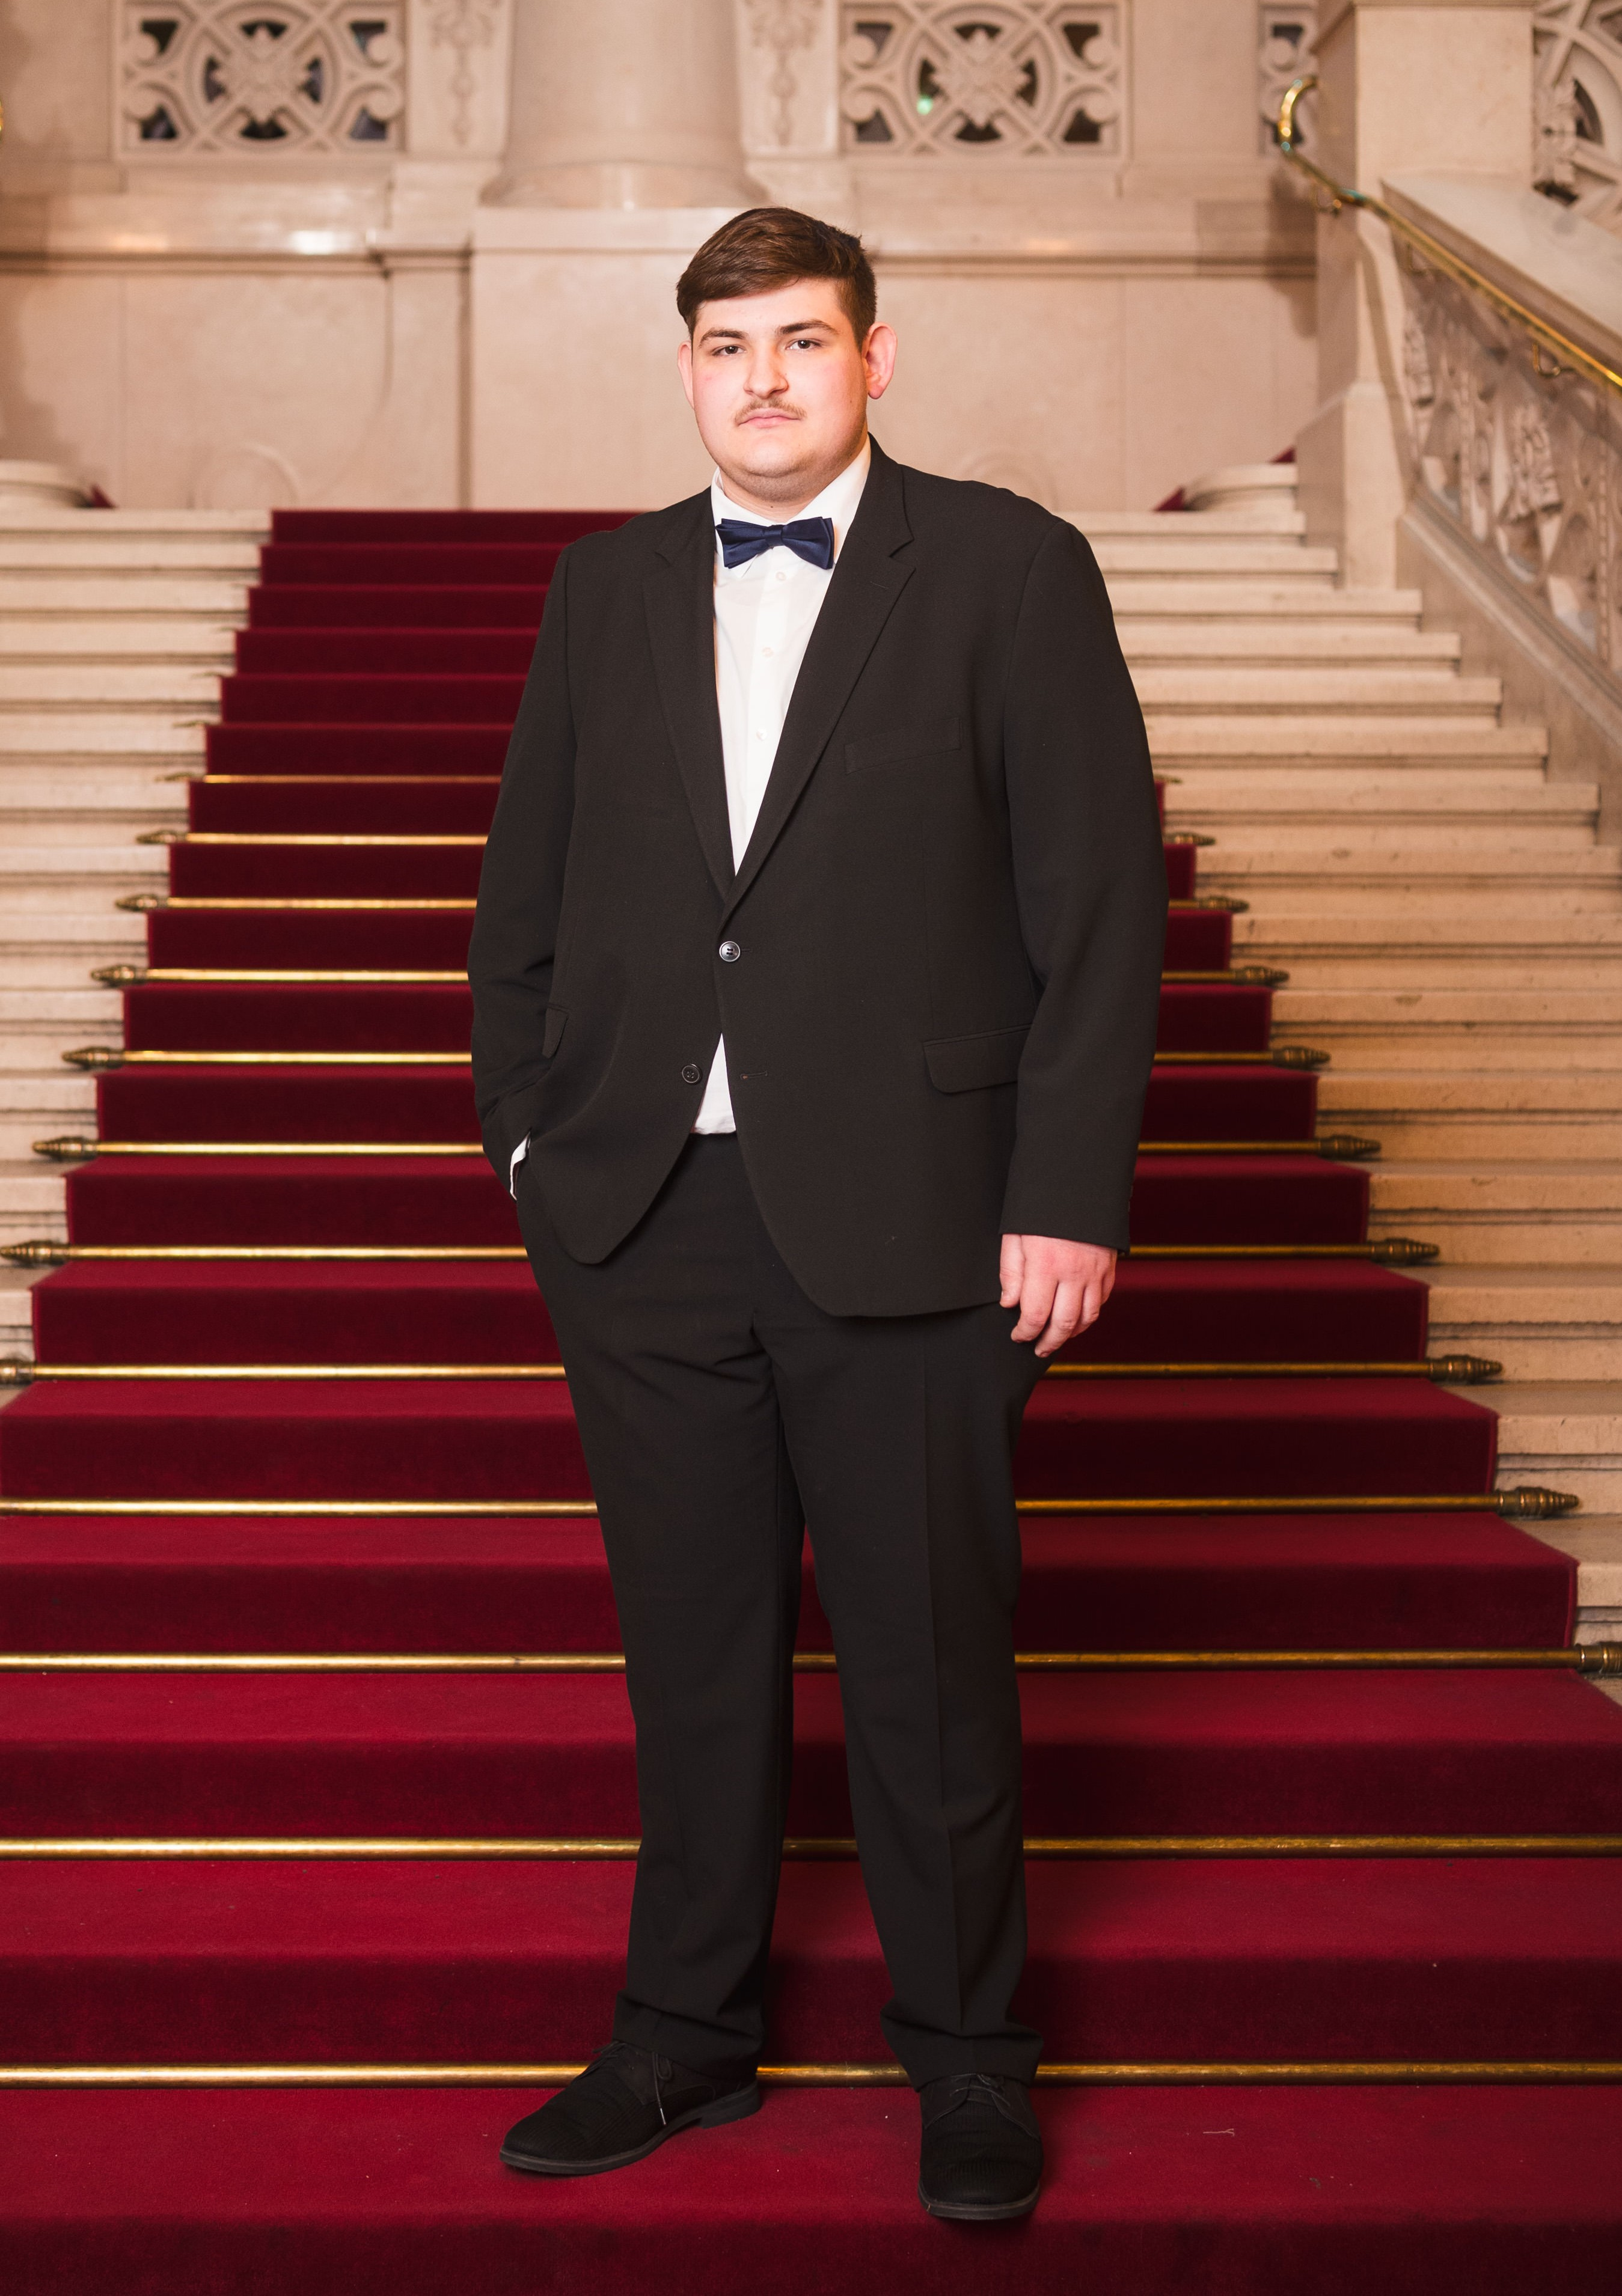
\includegraphics[width=\linewidth]{Pictures/daniel}
				\captionof{figure}{Porträt \\Daniel Schauer}
				\label{fig:daniel}
			\end{minipage}
			\hfill
			\begin{minipage}{0.65\textwidth}
				\vspace{-40pt}
				\textbf{Daniel Schauer: OnBoard-Software}
				\begin{itemize}
					\item Projektleiter \vspace{-10pt}
					\item Verbindung von Software und Hardware (ESP32 zu Sensoren) \vspace{-10pt}
					\item Kamera-Übertragung zur Web-Oberfläche \vspace{-10pt}
					\item Umsetzung einer schwenkbaren Kamera \vspace{-10pt}
					\item Dokumentation \vspace{-10pt}
				\end{itemize}
			\end{minipage} \\[1cm]
		
			%Simon---------------------------
			\begin{minipage}{0.18\textwidth}
				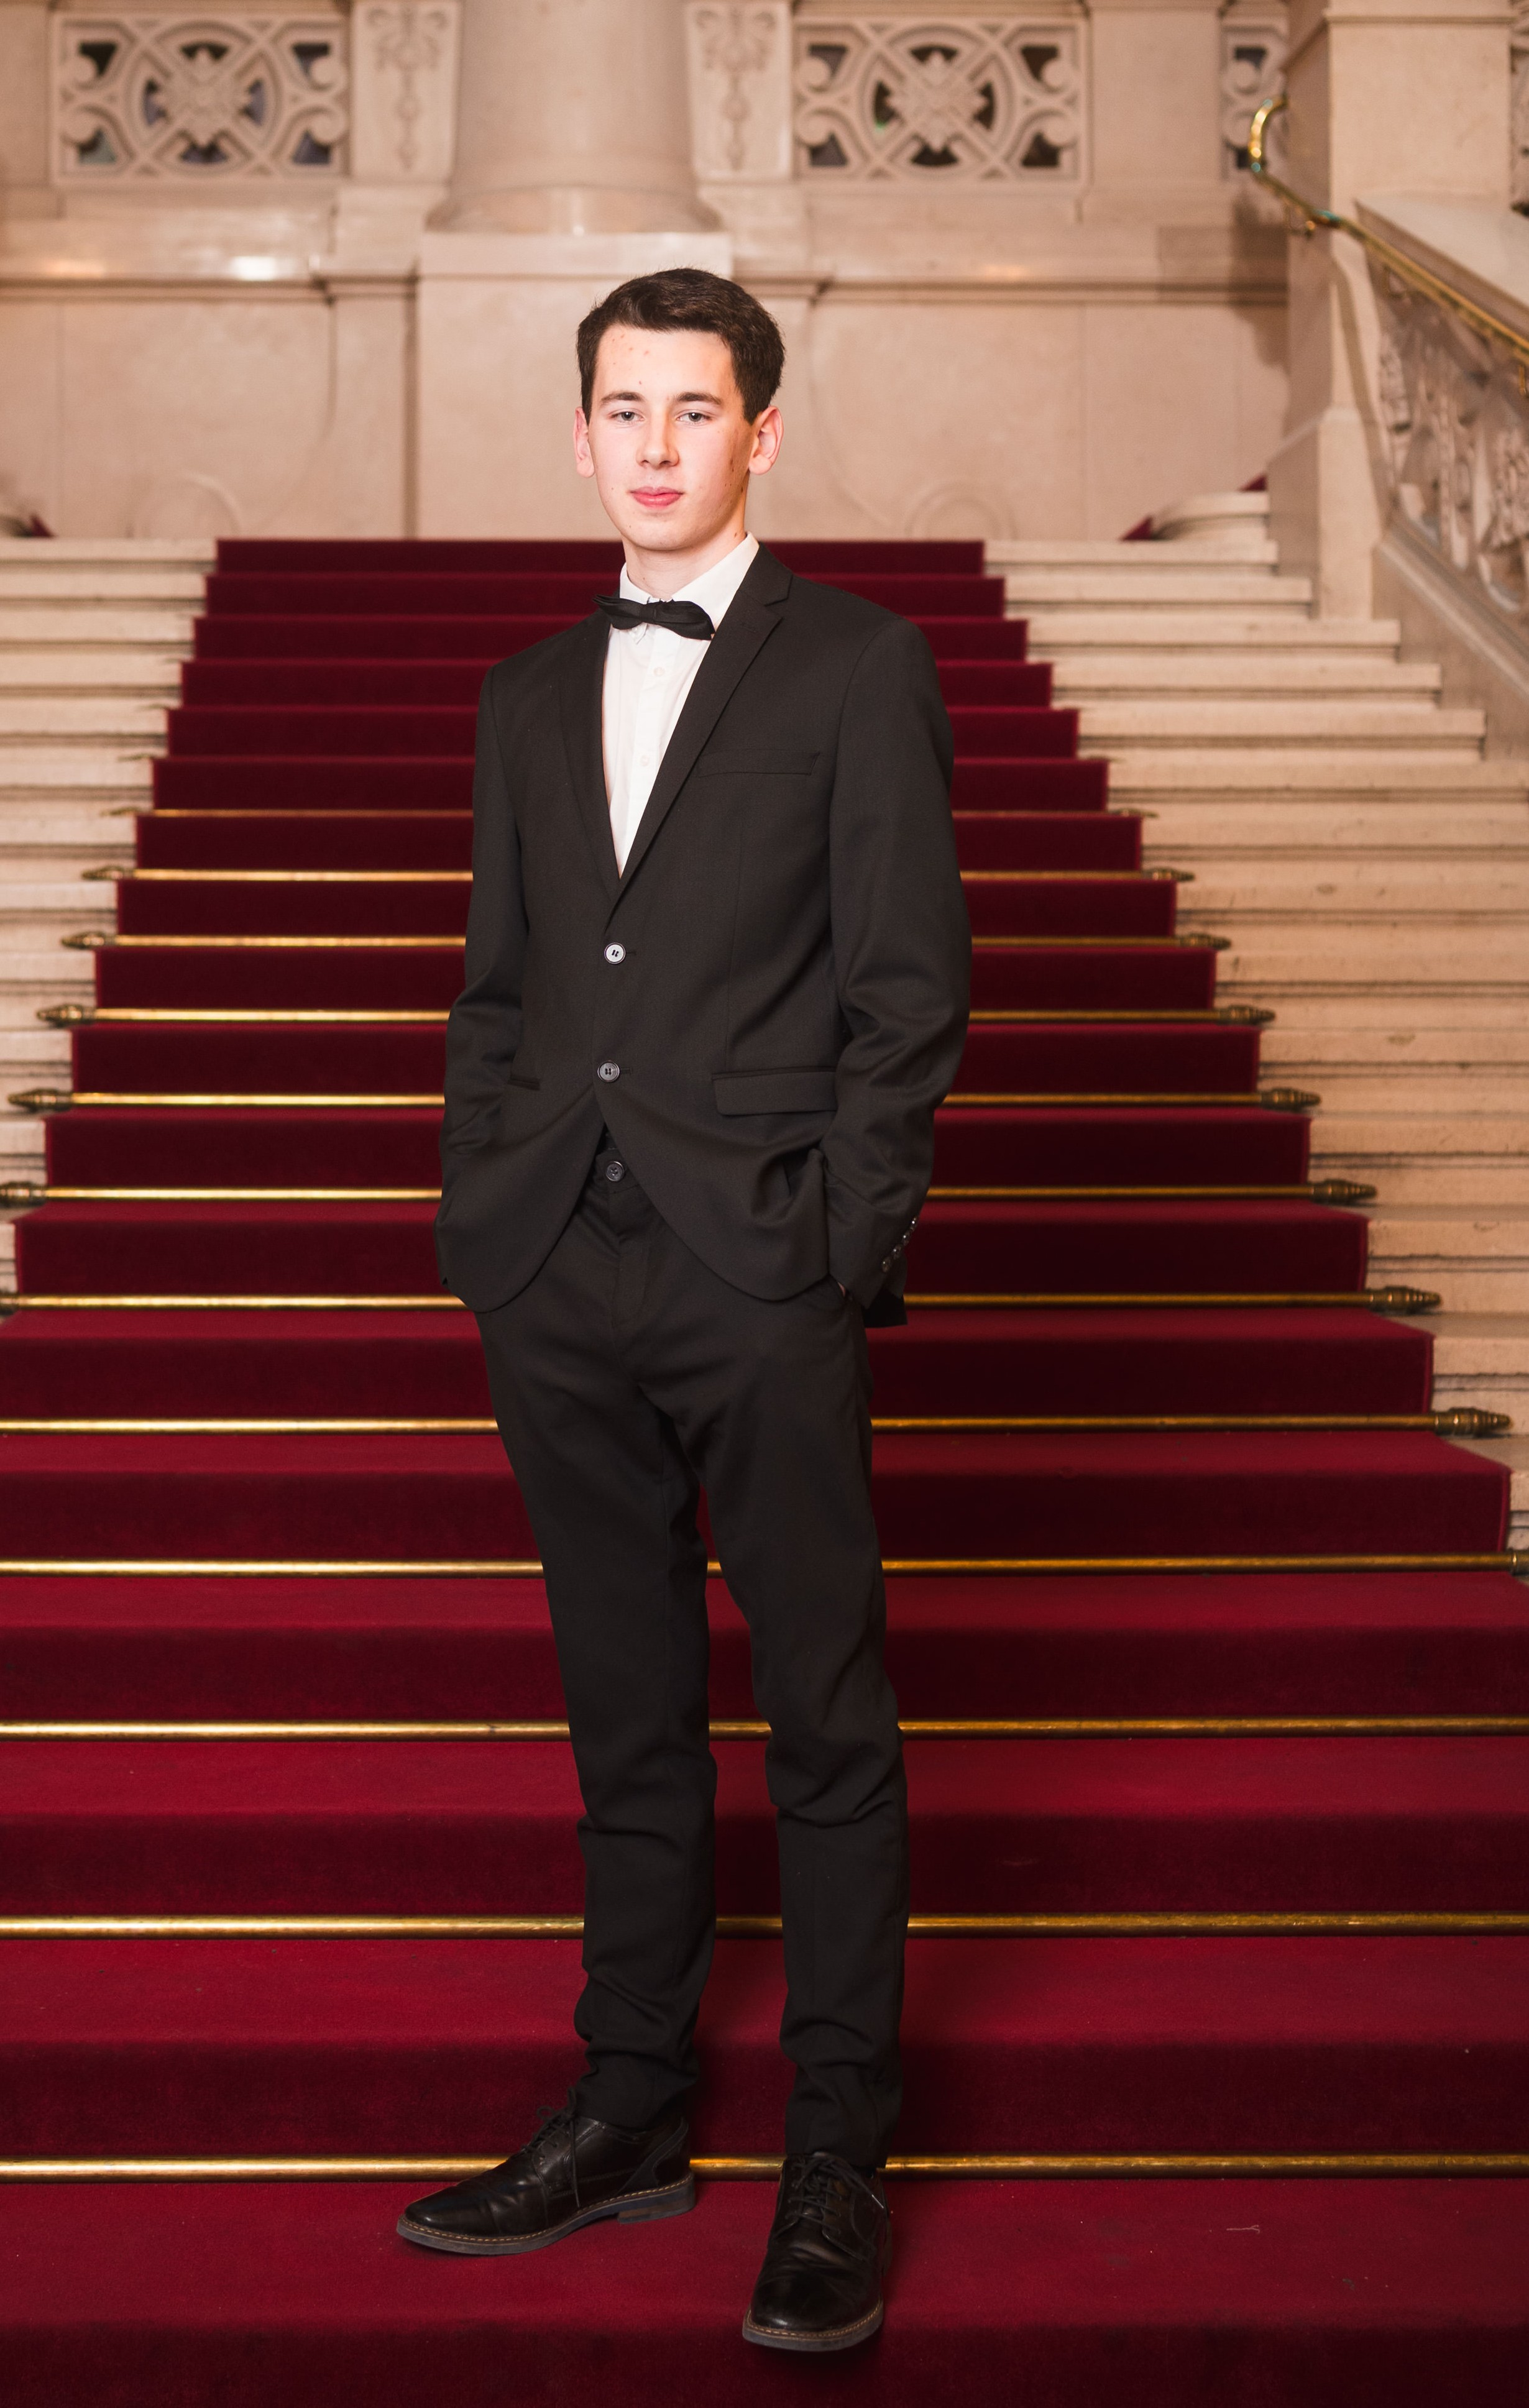
\includegraphics[width=\linewidth]{Pictures/spari}
				\captionof{figure}{Porträt \\Simon Spari}
				\label{fig:simon}
			\end{minipage}
			\hfill
			\begin{minipage}{0.65\textwidth}
				\vspace{-20pt}
				\textbf{Simon Spari: Software-App}
				\begin{itemize}
					\item Benutzeroberfläche (Web-Oberfläche) für Steuerung \vspace{-10pt}
					\item Übertragung der Steuerung/Befehle von Web-Oberfläche zu ESP32 \vspace{-10pt}
					\item Kamera Visualisierung auf der Website
					\item Dokumentation \vspace{-10pt}
				\end{itemize}
			\end{minipage} \\[1cm]
			%Felix---------------------------
			\begin{minipage}{0.18\textwidth}
				
\includegraphics[width=\linewidth]{Pictures/felix}
				\captionof{figure}{Porträt Felix Hochegger}
				\label{fig:felix}
			\end{minipage}
			\hfill
			\begin{minipage}{0.65\textwidth}
				\vspace{-60pt}
				\textbf{Felix Hochegger: Hardware-Design und Mechanik}
				\begin{itemize}
					\item ESEL
					\item Bau des Roboter Gehäuses \vspace{-10pt}
					\item Ansteuerung und Verbindung von Hardware (Ansteuerung und Berechnung der Motoren) \vspace{-10pt}
					\item Dokumentation \vspace{-10pt}
				\end{itemize}
			\end{minipage}
			\end{center}
			\newpage
		\subsection{Projektstrukturplan} %Daniel
		Unsere Diplomarbeit beschäftigt sich mit der Entwicklung eines Lastenroboters. Der Lastenroboter soll etwa ein Gewicht von 25 Kilogramm tragen können. Die Steuerung erfolgt über eine Website, und zusätzlich soll eine Kamera eingebaut werden. Im Lastenroboter wird auch eine Waage eingebaut, damit man sehen kann, wie schwer die transportierte Last ist. \\ Das Ziel dieser Diplomarbeit ist also, ein betriebsbereiter Prototyp eines Lastenroboters mit Kamerasystem und Waage zu entwickeln und zu realisieren. \\[0.4cm]
		\textbf{Geplantes Ergebnis der individuellen Themenstellungen:} \\
		\textbf{Felix Hochegger:}
		Bau des Roboter-Gehäuses und Integration der Komponenten, Verbindung der Hardware im besonderen Ansteuerung der Motoren \\
		\textbf{Simon Spari:}
		Entwicklung einer Benutzeroberfläche (Web-Oberfläche) zur Steuerung des Roboters, Übertragung der Steuerbefehle in Echtzeit an die Hardware \\
		\textbf{Daniel Schauer:}
		Verbindung von Software und Hardware zur Umsetzung der Steuerbefehle, Kamera-Übertragung in Echtzeit zur GUI, Umsetzung schwenkbare Kamera\\[0.4cm]
		\textbf{Projektstrukturplan:} \\
		Um unser Projekt besser zu strukturieren, haben wir am Anfang einen Grobplan für den Lastenroboter erstellt. Er hilft uns, die einzelnen Aufgaben und deren Verknüpfungen besser zu definieren. So können wir sicherstellen, dass Mechanik, Hardware und Software ohne Probleme zusammenarbeiten. Durch diese Planung behalten wir den Überblick über unser Projekt.
		\begin{center}
			\begin{minipage}{\textwidth}
				\centering
				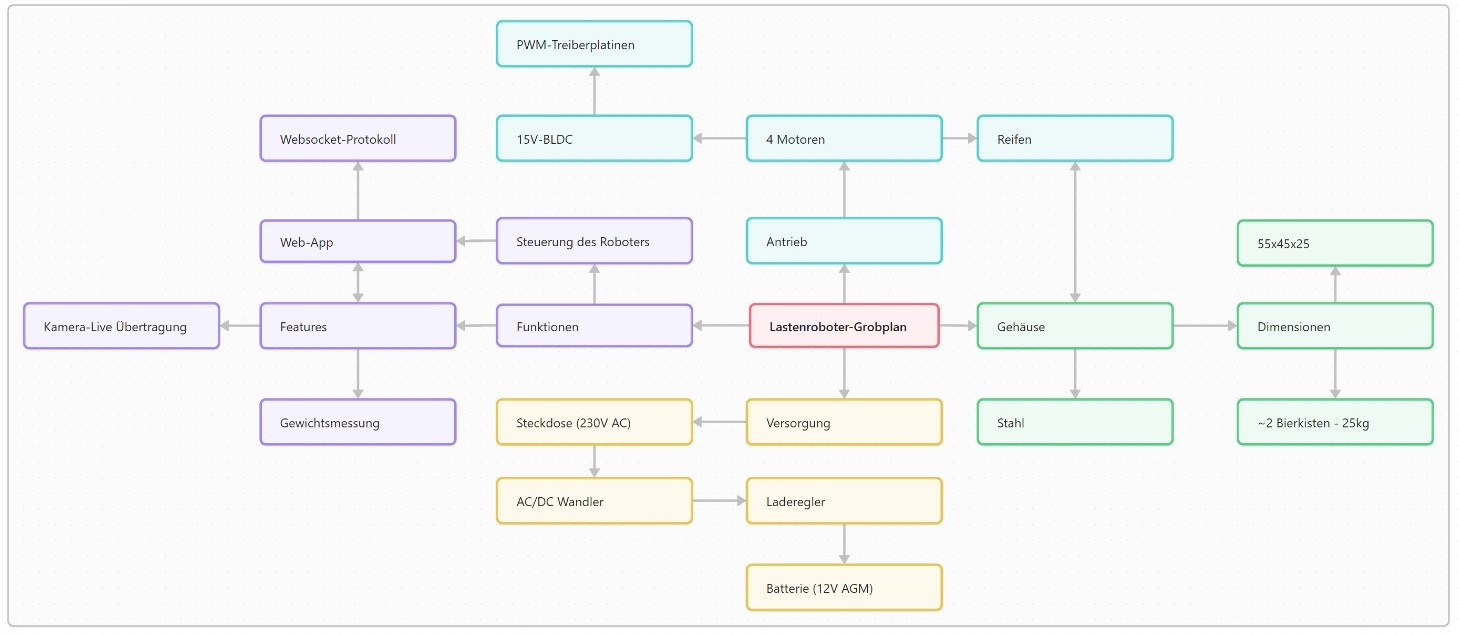
\includegraphics[scale=0.42]{Pictures/Projekt-Grobplan}
				\captionof{figure}{Lastenroboter Projekt-Grobplan}
				\label{fig:sprojekt_grobplan}
				\vspace{-4pt}
				{\small Quelle: eigene Abbildung erstellt mit Obsidian}
			\end{minipage}
		\end{center}
		\newpage
		\subsection{Meilensteine} %Daniel
		Um unseren Fortschritt und unsere Zeiteinteilung besser im Überblick zu behalten, wurden bestimmte Meilensteine für das Projekt definiert. Diese sind sehr hilfreich, um das Projekt strukturiert umzusetzen, angefangen von der Projektplanung bis hin zum fertigen Prototyp. \\[0.5cm]
		Die folgenden Meilensteine wurden bei der Projektplanung definiert:
		\begin{longtable}{| l | l |}
			\hline
			\textbf{Meilenstein} & \textbf{Datum} \\
			\hline
			\endfirsthead
			\hline
			\textbf{Meilenstein} & \textbf{Datum} \\
			\hline
			\endhead
			\hline
			Grundlegendes Gehäuse & 07.11.2024 \\
			\hline
			Funktionsfähige Website & 19.12.2024 \\
			\hline
			Funktionsfähige steuerbare Motoren & 16.01.2025 \\
			\hline
			Funktionsfähiger Prototyp & 06.03.2025 \\
			\hline
		\end{longtable}
		\subsection{Kostenaufstellung} %Daniel
			\begin{center}
				\begin{longtable}{| p{8.2cm} | r | r | r |}
					\hline
					\textbf{Artikel} & \textbf{Einzelpreis} & \textbf{Stückzahl} & \textbf{Gesamt} \\
					\hline
					\endfirsthead
					\hline
					\textbf{Artikel} & \textbf{Einzelpreis} & \textbf{Stückzahl} & \textbf{Gesamt} \\
					\hline
					\endhead
					\hline
					Aufblasbares Rad 10'' 260x85  & 16.70 € & 4 & 66.80 € \\ \hline
					MCP23017 GPIO Expander-Board & 4.54 € & 2 & 9.08 € \\ \hline
					PICAA LED Arbeitsscheinwerfer & 6.55 € & 2 & 13.10 € \\ \hline
					2 Stück PWM Motor Steuerung Treiber Platinen & 35.78 € & 2 & 71.56 € \\ \hline
					Micro Servo Motor SG90 & 6.04 € & 1 & 6.04 € \\ \hline
					IRM-30-15ST AC/DC-Leistungsmodul & 17.04 € & 1 & 17.04 € \\ \hline
					SOLSUM 0808 Solarladeregler & 25.17 € & 1 & 25.17 € \\ \hline
					Platinen & 37.14 € & 1 & 37.14 € \\ \hline
					ESP32-CAM & 13.70 € & 1 & 13.70 € \\ \hline
					12 Stück Halbbrücken Wägezelle & 11.09 € & 1 & 11.09 € \\ \hline
					ESP32 & 11.09 € & 1 & 11.09 € \\ \hline
					Dunkermotoren & 65.00 € & 2 & 130.00 € \\ \hline
					AGM 12V Batterie & 24.80 € & 1 & 24.80 € \\ \hline
					Diverse Kleinteile & 30.00 € & 1 & 30.00 € \\ \hline
					\textbf{Summe} & & & \textbf{466.61 €} \\
					\hline
				\end{longtable}
			\end{center}
			\newpage
	\section{Antrieb}
	
		\subsection{Motoren} %Felix
		
			\subsubsection{Übersicht}
			Für den Antrieb des Lastenroboters werden BLDC-Motoren eingesetzt. Verwendet werden die BLDC-Motoren von Dunkermotoren (Typ BG 40X25). Ein BLDC-Motor auch bürstenloser Gleichstrommoter gennant, wird über drei Phasen betrieben. Der BLDC-Motor wird oft in der Industrie eingesetzt, da er eine hohe Leistung bietet.
			
			\begin{center}
				\begin{minipage}{\textwidth}
					\centering
					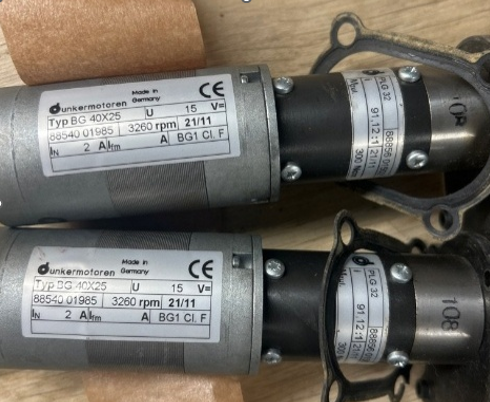
\includegraphics[scale=0.5]{Pictures/Motoren}
					\captionof{figure}{Motoren}
					\label{fig:spiffs_init}
					\vspace{-2pt}
					{\small Quelle: eigene Abbildung}
				\end{minipage}
			\end{center}
			
			\subsubsection{Funktionsweise}
			Die Funktionsweise eines bürstenlosen Gleichstrommotors basiert auf der Wechselwirkung zwischen dem Magnetfeld des Stators und dem Magnetfeld des Rotors.\\[0.5cm]
			\textbf{Stator:} Der Stator besteht aus mehreren Spulen, die üblicherweise drei Phasen umfasst. Die drei Phasen werden mit Wechselstrom angesteuert die dann ein rotierendes Magnetfeld erzeugen.\\[0.5cm]
			\textbf{Rotor:} Der Rotor besteht aus einem Permanentmagneten. Dadurch das die Spulen ein rotierendes Magnetfeld erzeugen dreht sich der Rotor synchron mit diesem Magnetfeld mit.
			
			\begin{center}
				\begin{minipage}{\textwidth}
					\centering
					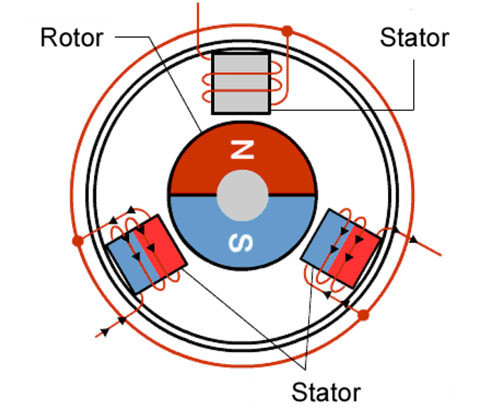
\includegraphics[scale=0.3]{Pictures/BLDC_Motor}
					\captionof{figure}{BLDC-Motor}
					\label{fig:spiffs_init}
					\vspace{-2pt}
					\small Quelle: www.elektrikrehberiniz.com
				\end{minipage}
			\end{center}
			Damit die Phasen des Motors korrekt geschaltet werden, muss die genaue Position des Rotors im Inneren des Motors erfasst werden. Die genaue Position des Rotors wird durch Hallsensoren erfasst. Die drei Hallsensoren geben diese Informationen an die Steuerelektronik weiter. Mit diesen Daten kann die optimale Beschaltung der Phasen berechnet werden.\\[0.5cm]
			Zur Steuerung der Drehzahl wird ein Pulsweitenmodulations-Signal (PWM-Signal) verwendet. Durch die PWM wird die Stromzufuhr zu den Phasen des Motors gesteuert. Wenn das Pulsweitenmodulations-Signal (PWM) erhöht wird, bedeutet das, dass die Phasen in kürzeren Abständen angesteuert werden. Dadurch erhält der Motor häufiger Energieimpulse, was zu einer höheren Drehzahl des Rotors führt. Das PWM-Signal regelt die Versorgungsspannung, indem es sie in schneller Folge ein- und ausschaltet. Je höher das Tastverhältnis des PWM-Signals, desto länger bleibt die Spannung während eines Zyklus eingeschaltet, wodurch der Motor mehr Energie erhält und sich schneller dreht.\\[0.5cm]
			Auf diese Weise kann der Motor effizient mit variabler Geschwindigkeit betrieben werden.
			
			\begin{center}
				\begin{minipage}{\textwidth}
					\centering
					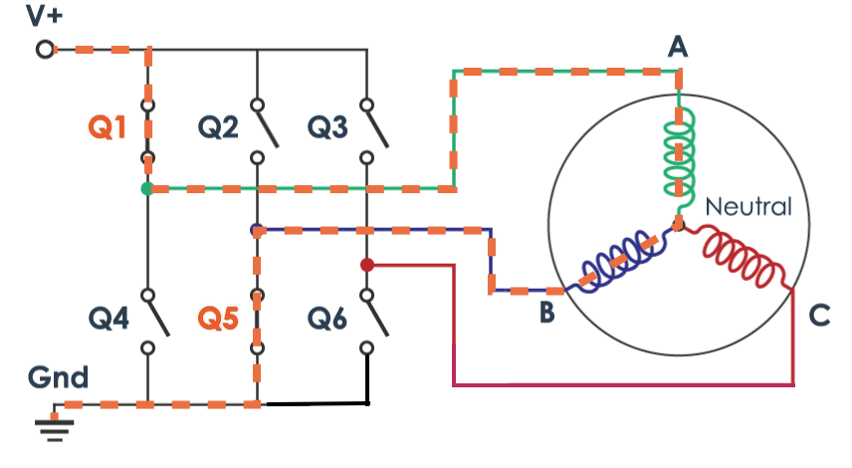
\includegraphics[scale=0.6]{Pictures/Phasen_steuerung}
					\captionof{figure}{Phasensteuerung}
					\label{fig:spiffs_init}
					\vspace{-2pt}
					\small Quelle: davincii.de/arduino-projekte/brushless-motor-ansteuerung
				\end{minipage}
			\end{center}
			
			\subsubsection{Technische Daten}
			
			\begin{tabular}{| l | l |}  
				\hline  
				\textbf{Eigenschaft} & \textbf{Wert} \\   
				\hline  
				Versorgungsspannung & 15V \\  
				\hline  
				Maximale Rotationsgeschwindigkeit der Antriebswelle & 3260 rpm \\  
				\hline  
				Max. Strom & 2A \\  
				\hline  
			\end{tabular}
			
		\subsection{Motorentreiber} %Felix
		
			\subsubsection{Überblick}
		Für die Ansteuerung der BLDC-Motoren wird der Motortreiber ZX-X11H verwendet. Dieser Motortreiber übernimmt die elektronische Kommutierung, das heißt dieser Treiber schaltet die Phasen des Motors damit sich der Rotor dreht. Die Rotorposition wird über Hallsensoren erfasst. Mit diesen Daten werden die Phasen richtig angesteuert. Dies ermöglichten einen gleichmäßigen Betrieb sowie eine exakte Regelung von Drehzahl und Drehmoment. Durch die integrierte PWM-Steuerung kann die Geschwindigkeit präzise eingestellt werden. Zusätzlich verfügt der ZS-X11H über eine Richtungssteuerung und einer Brems-Funktion.
		
			\subsubsection{Aufbau und Funktionen}
			
		\begin{center}
			\begin{minipage}{\textwidth}
				\centering
				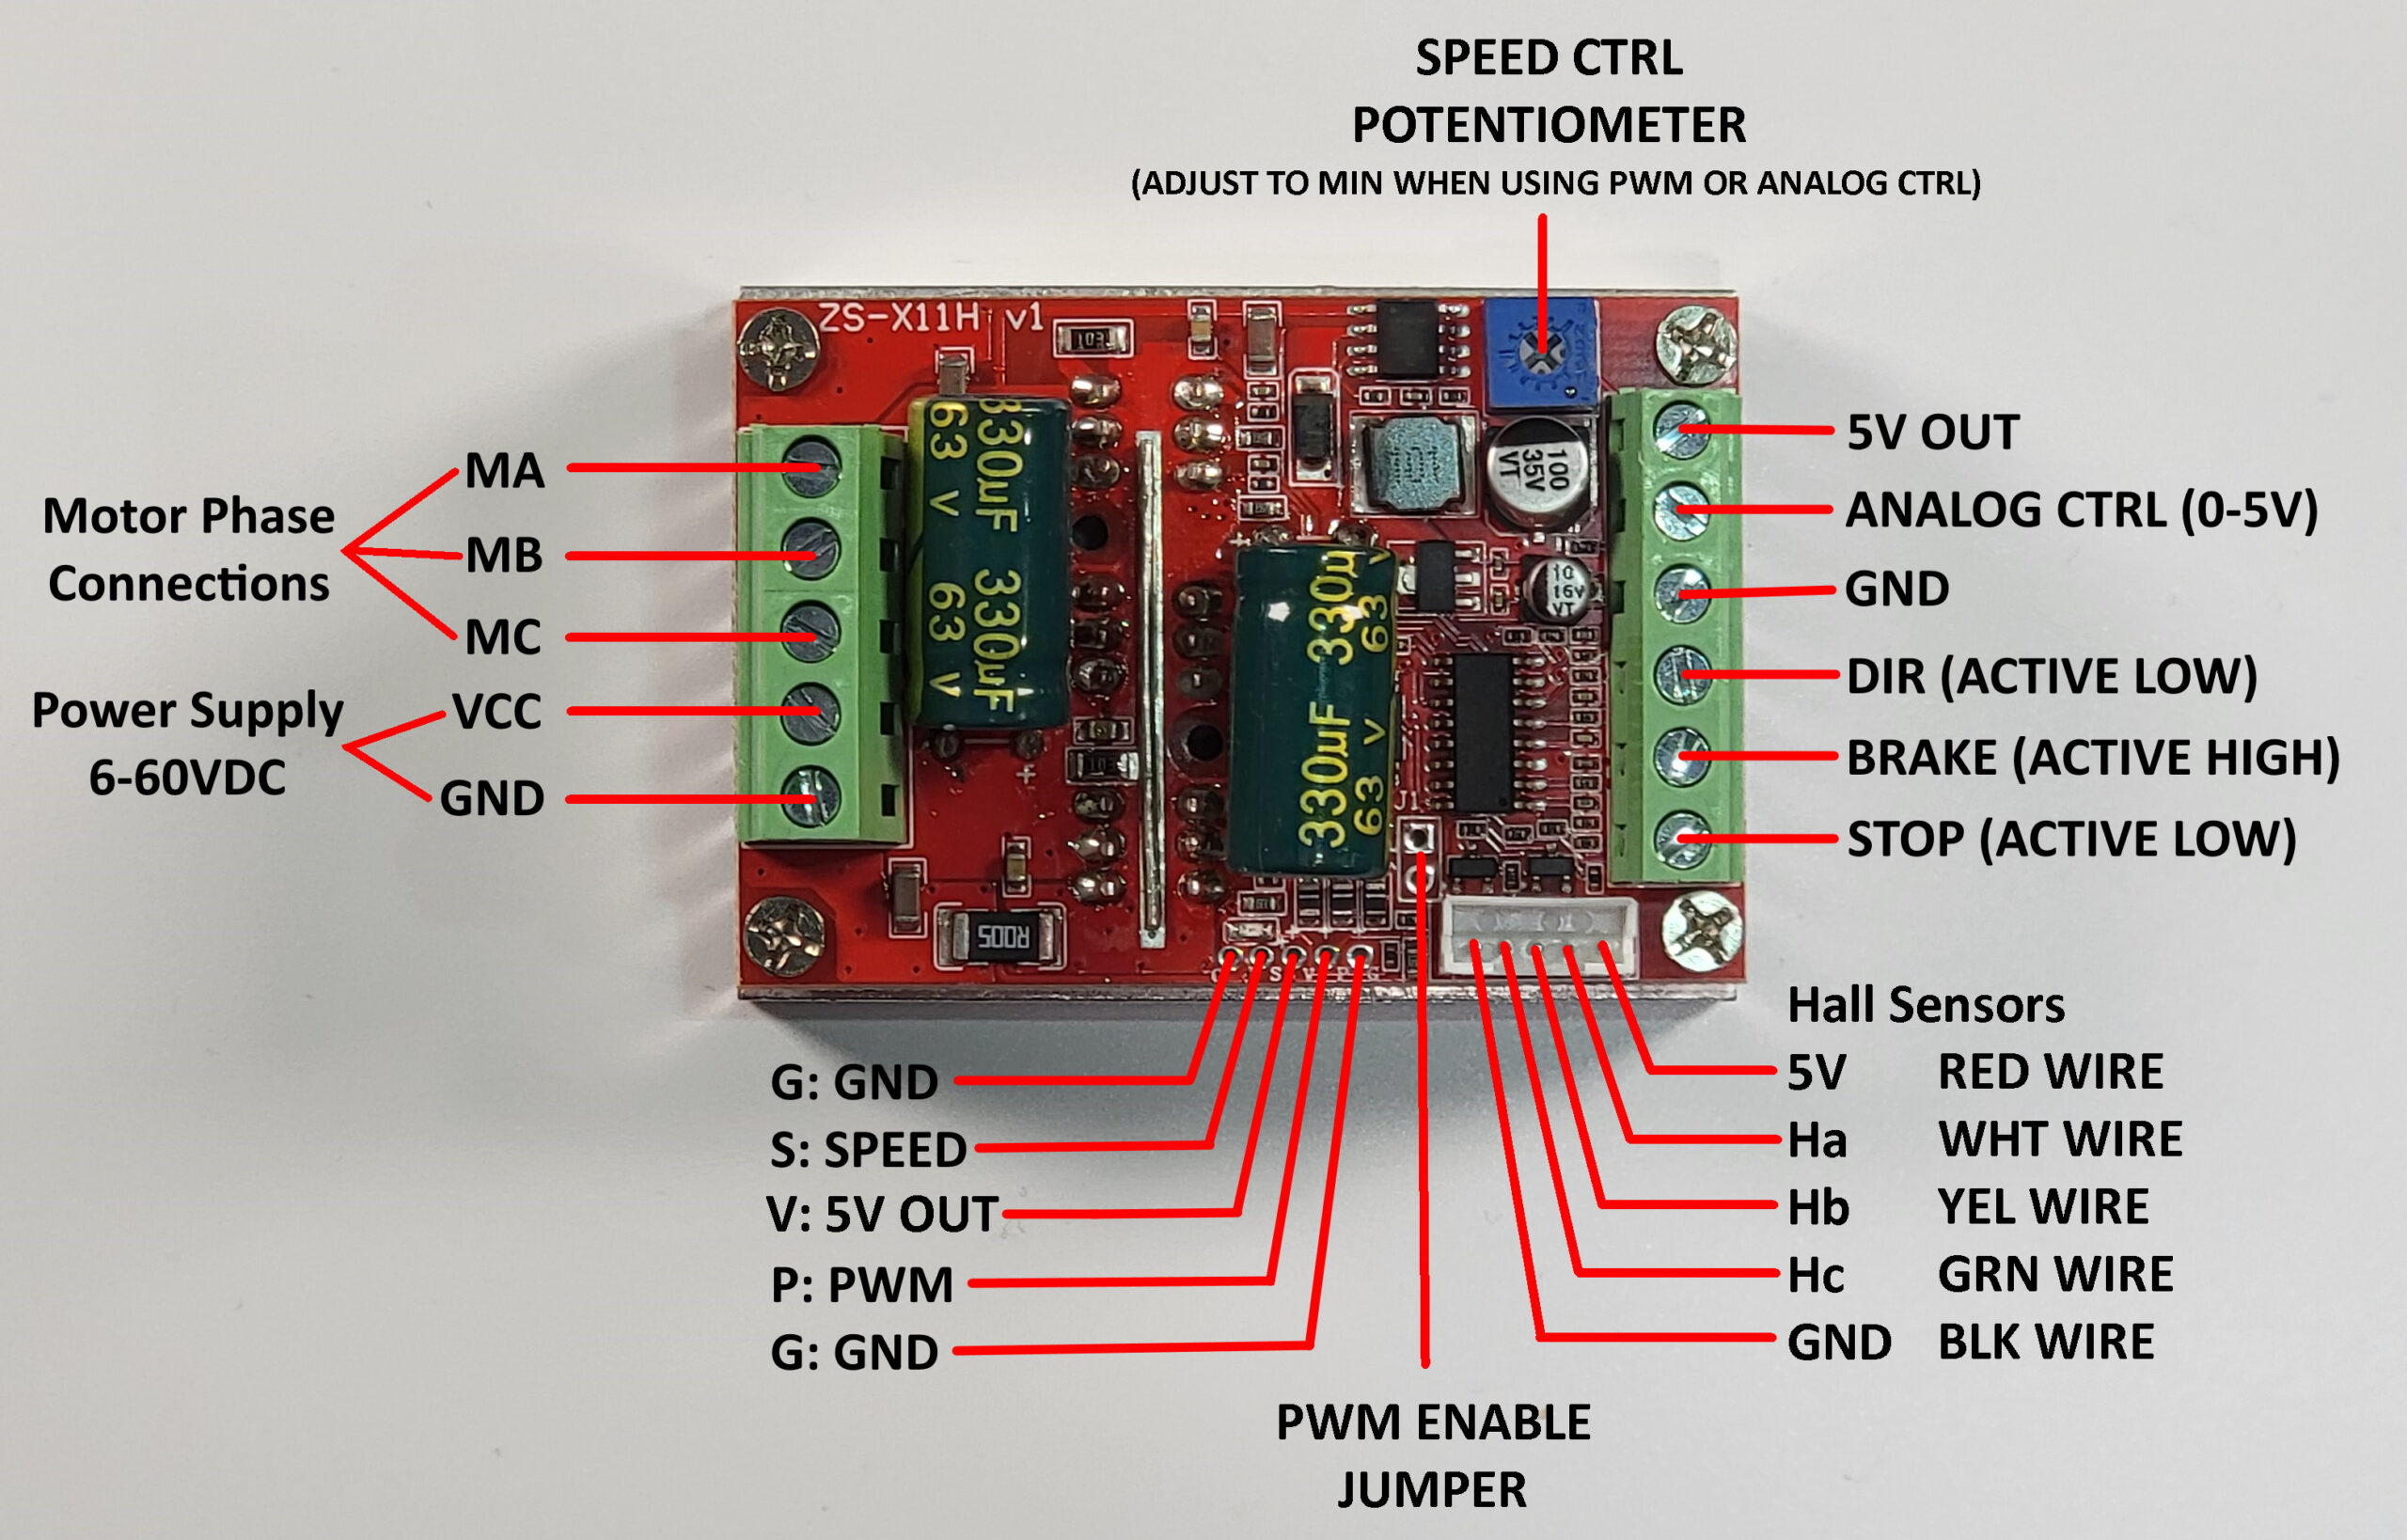
\includegraphics[scale=0.15]{Pictures/ZS-X11H}
				\captionof{figure}{Motorteiber-ZS-X11H}
				\label{fig:spiffs_init}
				\vspace{-2pt}
				\small Quelle: mad-ee.com/easy-inexpensive-hoverboard-motor-controller/g
			\end{minipage}
		\end{center}
		\newpage
		\subsubsection*{Steuerung der Phasenströme:}
		Der Treiber steuert die drei Motorphasen (MA, MB, MC) mithilfe eines integrierten MOSFET-Brückenschaltkreises. Mit den Daten der Hallsensoren schaltet der Treiber die Phasen damit sich der Rotor mit der gewünschten Geschwindigkeit dreht.
		
		\begin{center}
			\begin{minipage}{\textwidth}
				\centering
				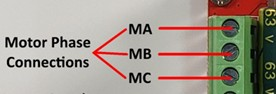
\includegraphics[scale=1]{Pictures/Motorphasen}
				\captionof{figure}{Motorphasen Verbindung}
				\label{fig:spiffs_init}
				\vspace{-2pt}
				\small Quelle: mad-ee.com/easy-inexpensive-hoverboard-motor-controller/g
			\end{minipage}
		\end{center}
		
		\subsubsection*{PWM-Steuerung}
		\begin{itemize}
			\item Die Pulsweitenmodulation (PWM) steuert die Geschwindigkeit des Motors, indem sie die Einschaltdauer der Spannung variiert, wodurch die durchschnittliche Leistung, die den Motorwicklungen zugeführt wird, angepasst wird.
			\item Die Amplitude des PWM-Signals muss zwischen 2,5-5 V liegen.
			\item Die PWM-Frequenz muss zwischen 50-20 kHz liegen.
			\item Die Platine ist ausgestattet mit einer externen und internen PWM-Steuerung.
			\item Wenn die Brücke auf der Platine verbunden wird, kommt die externe PWM zum Einsatz.
		\end{itemize}
		
		\begin{center}
			\begin{minipage}{\textwidth}
				\centering
				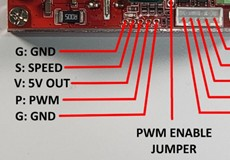
\includegraphics[scale=1]{Pictures/PWM-Treiber}
				\captionof{figure}{Pins für die PWM}
				\label{fig:spiffs_init}
				\vspace{-2pt}
				\small Quelle: mad-ee.com/easy-inexpensive-hoverboard-motor-controller/g
			\end{minipage}
		\end{center}
		\newpage
		\subsubsection*{Richtungswechsel und Bremse}
		\begin{itemize}
			\item Die Platine verfügt über zwei Steuereingänge ein für Richtungswechsel (DIR) und eine Bremsfunktion (BRAKE).
			\item Der Richtungswechsel erfolgt, indem das Signal bei dem Eingang von LOW auf HIGH oder umgekehrt wechselt. Das Umschalten der Richtung wechselt die Reihenfolge der Phasenströme, wodurch sich dann der Motor in die andere Richtung dreht.
			\item Die Bremse reagiert auf ein HIGH-Signal. Das heißt wenn am Eingang ein HIGH-Signal angelegt wird, stoppt der Motor, indem die Wicklungen kurzgeschlossen werden.
		\end{itemize}
		
		\begin{center}
			\begin{minipage}{\textwidth}
				\centering
				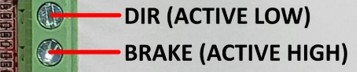
\includegraphics[scale=1]{Pictures/Bremse-Richtungswechsel}
				\captionof{figure}{Pin für die Bremse und den Richtungswechsel}
				\label{fig:spiffs_init}
				\vspace{-2pt}
				\small Quelle: mad-ee.com/easy-inexpensive-hoverboard-motor-controller/g
			\end{minipage}
		\end{center}
		
		\subsubsection*{Spannungs- und Stromversorgung}
		\begin{itemize}
			\item Der Treiber kann mit einer Versorgungsspannung von 12V-60V betrieben werden, wodurch er für eine Vielzahl von BLDC-Motoren geeignet ist.
			\item Die maximale Stromaufnahme des Treibers liegt bei zirka 15A.
			\item Der Treiber ist für Motoren bis zu 500 Watt geeignet und kann damit leistungsstarke Motoren betreiben
		\end{itemize}
		
		\begin{center}
			\begin{minipage}{\textwidth}
				\centering
				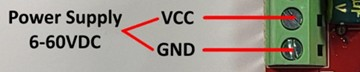
\includegraphics[scale=1]{Pictures/Versorgung}
				\captionof{figure}{Versorgungs-Pins}
				\label{fig:spiffs_init}
				\vspace{-2pt}
				\small Quelle: mad-ee.com/easy-inexpensive-hoverboard-motor-controller/g
			\end{minipage}
		\end{center}
		
		\newpage
		
		\begin{minipage}{\textwidth}
		\subsubsection*{Hall-Sensoren}
		\begin{itemize}
			\item Der Treiber verwendet drei Hall-Sensor-Eingänge. (Ha, Hb, Hc)
			\item Mit diesen Hall-Sensoren wird die Rotorposition ermittelt damit die Phasen des Motors richtig geschaltet werden.
			\item Die Sensoren ermöglichen eine effiziente und stabile Steuerung.\\[0.5cm]
		\end{itemize}
		\end{minipage}
		
		\begin{minipage}{\textwidth}
			\centering
			\includegraphics[scale=1]{Pictures/Hall-sensoren Eingänge}
			\captionof{figure}{Hall-sensoren Eingänge}
			\label{fig:spiffs_init}
			\vspace{-2pt}
			\small Quelle: mad-ee.com/easy-inexpensive-hoverboard-motor-controller/g
		\end{minipage}
		
		\subsubsection*{Sicherheit und Schutzfunktionen}
		\begin{itemize}
			\item Der Treiber verfügt über einen Überstrom- und Überspannungsschutz damit der Motor und die Elektronik geschütz ist.
			\item Ein thermischer Schutz verhindert Schäden durch Überhitzung.
		\end{itemize}
		\newpage
		\subsection{Schaltungsaufbau mit einem Motor} %Felix
		
			\subsubsection{Komponenten}
			\begin{itemize}
				\item BLDC-Motor
				\item Motortreiber (ZS-X11H)
				\item Mikrocontroller (ESP32)
				\item Expander Modul (MCP23017)
			\end{itemize}
			
			\subsubsection{Schaltungsaufbau und Verbindungen}
			\begin{minipage}{\textwidth}
				\centering
				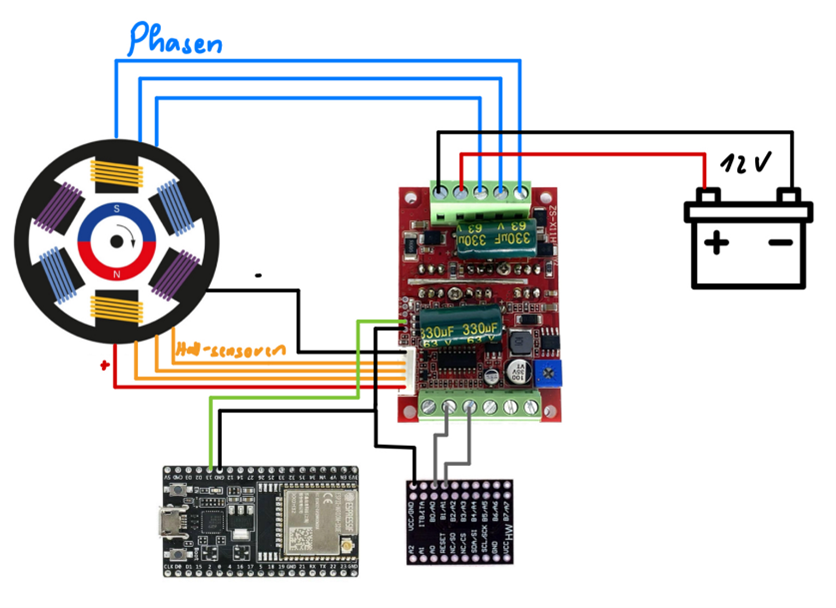
\includegraphics[scale=1.5]{Pictures/Schaltungsaufbau-1Motor}
				\captionof{figure}{Schaltungsaufbau mit einem Motor}
				\label{fig:spiffs_init}
				\vspace{-2pt}
				\small Quelle: eigene Abbildung
			\end{minipage}
			\newpage
			\subsubsection*{Phasenanschlüsse des Motors (blau):}
			
			Die Phasen des Motors werden mit der Treiberplatine verbunden. Diese werden abwechselnd mit Spannung versorgt, um eine Drehbewegung zu erzeugen. Die weiße Phase des Motors wird mit MA verbunden. Die blaue Phase des Motors wird mit MB verbunden. Die orange Phase des Motors wird mit MC verbunden. \\[0.5cm]
			
			\begin{minipage}{0.48\textwidth} % Erste Minipage für das erste Bild
				\raggedright
				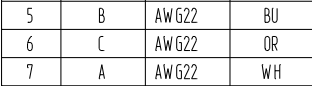
\includegraphics[scale=0.5]{Pictures/Phasen-motor}
				\captionof{figure}{\raggedright Hall-Sensoren Eingänge}
				\label{fig:phasen_motor}
				\vspace{-2pt}
				\small Quelle: easy-inexpensive-hoverboard-motor-controller
			\end{minipage}
			\hfill % Fügt Abstand zwischen den Bildern ein
			\begin{minipage}{0.48\textwidth} % Zweite Minipage für das zweite Bild
				\raggedright
				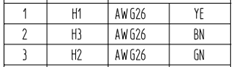
\includegraphics[scale=0.5]{Pictures/Hall-Sensoren-Motor}
				\captionof{figure}{\raggedright Hall-Sensoren-Motor}
				\label{fig:phasen_treiber}
				\vspace{-2pt}
				\small Quelle: eigene Abbildung
			\end{minipage}
			
			\subsubsection*{Hall-Sensoren Verbindungen (orange)}
			
			Die Hall-Sensoren des Motors werden mit der Treiberplatine verbunden und erfassen die aktuelle Rotorposition. Diese Informationen werden an die Steuerelektronik übermittelt, die daraufhin die Motorphasen entsprechend schaltet, um die gewünschte Drehbewegung zu erzeugen. Dabei wird der gelbe Hall-Sensor mit HA, der grüne mit HB und der braune mit HC auf dem Treiber verbunden. \\[0.5cm]
			
			\begin{minipage}{0.48\textwidth} % Erste Minipage für das erste Bild
				\raggedright
				\includegraphics[scale=0.5]{Pictures/Hall-sensoren Eingänge}
				\captionof{figure}{\raggedright Motor Phasen}
				\label{fig:phasen_motor}
				\vspace{-2pt}
				\small Quelle: eigene Abbildung
			\end{minipage}
			\hfill % Fügt Abstand zwischen den Bildern ein
			\begin{minipage}{0.48\textwidth} % Zweite Minipage für das zweite Bild
				\raggedright
				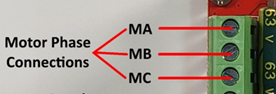
\includegraphics[scale=0.5]{Pictures/Phasen-treiber}
				\captionof{figure}{\raggedright Treiber Phasen}
				\label{fig:phasen_treiber}
				\vspace{-2pt}
				\small Quelle: eigene Abbildung
			\end{minipage}
			
			\subsubsection*{Versorgung (rot und schwarz)}
			\begin{itemize}
				\item Der Treiber wird mit 12 Volt von der Batterie versorgt.
				\item Mit diesen 12 Volt steuert der Treiber den Motorstrom an den Phasen.
			\end{itemize}
			
			\begin{minipage}{\textwidth}
				\centering
				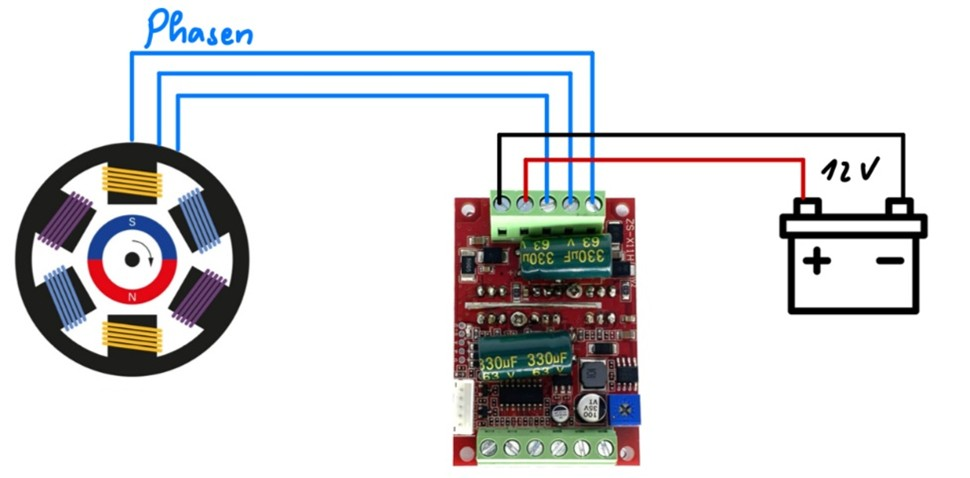
\includegraphics[scale=0.5]{Pictures/Versorgung-motor}
				\captionof{figure}{Versorgung der Motoren und Treiberplatine}
				\label{fig:spiffs_init}
				\vspace{-2pt}
				\small Quelle: eigene Abbildung
			\end{minipage}
			
			\subsubsection*{Steuerverbindung (grün und grau)}
			
			 Der ESP32 ist mit dem Motortreiber verbunden, um Geschwindigkeit zu regeln. Das funktioniert über ein PWM-Signal. \\[0.5cm]
			 Das Expander Modul steuert die Richtung und die Bremsfunktion. Der Richtungswechsel erfolgt, indem das Expander Modul den entsprechenden Eingang auf LOW oder HIGH schaltet. Die Bremse reagiert auf eine HIGH Signal. Das heißt, wenn das Expander Modul den Eingang auf der Steuerplatine HIGH schaltet, wird der Motor gebremst.
			 \\[0.5cm]
			
			\begin{minipage}{\textwidth}
				\centering
				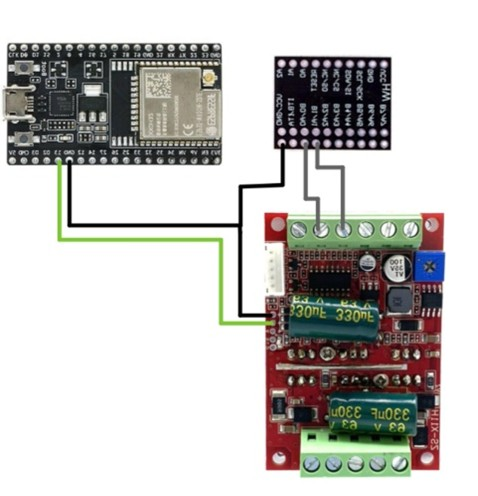
\includegraphics[scale=1]{Pictures/Steuerverbindung}
				\captionof{figure}{Ansteuerung der Treiberplatine}
				\label{fig:spiffs_init}
				\vspace{-2pt}
				\small Quelle: eigene Abbildung
			\end{minipage}
			
		\subsection{Schaltungsaufbau mit vier Motor} %Felix
			
			\subsubsection{Komponenten}
			\begin{itemize}
				\item 4 BLDC-Motor
				\item 4 Motortreiber (ZS-X11H)
				\item Mikrocontroller (ESP32)
				\item Expander Modul (MCP23017)
			\end{itemize}
			\newpage
			
			\subsubsection{Schaltungserweiterung für vier Motoren:}
			Der Lastenroboter wird von vier BLDC-Motoren angetrieben, die jeweils über einen eigenen Motortreiber gesteuert werden. Jeder Motortreiber wird über einen PWM-Pin des Esp32 verbunden, um die Geschwindigkeit zu regulieren. Zusätzlich wird jeder Motortreiber über das Expander-Modul angesteuert, um die Richtung zu ändern und die Bremse zu aktivieren. Alle Treiber werden mit 12 Volt von der Batterie versorgt. \\[0.5cm]
			\begin{minipage}{\textwidth}
				\centering
				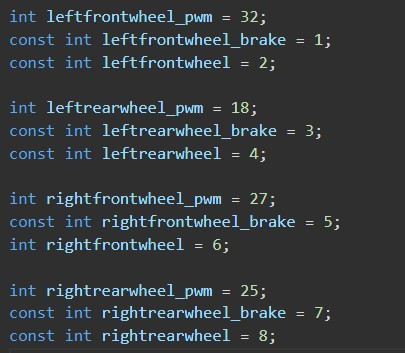
\includegraphics[scale=1.05]{Pictures/code_pins_motoren}
				\captionof{figure}{Motoren-GPIO Konfiguration}
				\label{fig:code_pins_motoren}
				\vspace{-2pt}
				\small Quelle: eigene Abbildung
			\end{minipage}
			
		\subsection{Code} 
		\subsubsection{Initialisierung}
		Um die Motoren beziehungsweise die Treiberplatinen anzusteuern, gibt es pro Motor drei Pins. Einer dieser Pins wird mit einem PWM-fähigen Pin am ESP32 verbunden. Die anderen beiden werden mit dem Expander Modul verbunden. Da das Expander Modul nur Digitale Ein-/Ausgänge besitzt, ist es nicht möglich die PWM-Signale auch über dieses Modul zu realisieren. Der Hauptgrund für diese Aufteilung auf den Expander ist, der das wir Analoge Pins am ESP32 einsparen müssen, um diese für andere Sensoren oder Aktoren einzusetzen. \\[0.5cm]
		\begin{minipage}{\textwidth}
			\centering
			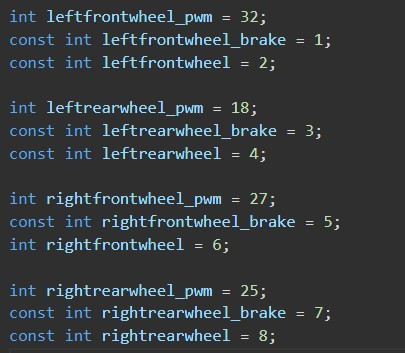
\includegraphics[scale=1.05]{Pictures/code_pins_motoren}
			\captionof{figure}{Motoren-GPIO Konfiguration}
			\label{fig:code_pins_motoren}
			\vspace{-2pt}
			\small Quelle: eigene Abbildung
			\vspace{20pt}
		\end{minipage}
		Um das Expander-Board zu nutzen, wird die Bibliothek Adafruit\_MCP23X17 verwendet. Diese Bibliothek ermöglicht eine einfachere Initialisierung und Ansteuerung der MCP-Pins, sodass die GPIOs ähnlich wie die des ESP32 genutzt werden können. Außerdem wird ein Objekt der Klasse Adafruit MCP23X17 erstellt, über das man später auf den Expander zugreifen kann. \\[0.5cm]
		\begin{minipage}{\textwidth}
			\centering
			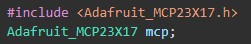
\includegraphics[scale=1.3]{Pictures/code_libary_motoren}
			\captionof{figure}{\texttt{Adafruit\_MCP23X17.h}-Bibliothek}
			\label{fig:code_libary_motoren}
			\vspace{-2pt}
			\small Quelle: eigene Abbildung
		\end{minipage}	
		\newpage
		\subsubsection{Setup-Code}
		Am Anfang des Setup-Codes wird überprüft, ob ein Expander Modul über die I2C Schnittstelle verbunden ist und dieses auch funktionstüchtig ist. Falls das nicht der Fall ist, wird ein Error über die Serielle Schnittstelle ausgegeben und das Setup wird unterbrochen. \\[0.5cm]
		\begin{minipage}{\textwidth}
			\centering
			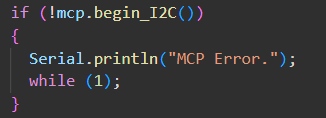
\includegraphics[scale=1.05]{Pictures/code_mcp_if_motoren}
			\captionof{figure}{MCP-Setup}
			\label{fig:code_mcp_if_motoren}
			\vspace{-2pt}
			\small Quelle: eigene Abbildung
			\vspace{10pt}
		\end{minipage}	
		Danach werden die Pins des ESP32 sowie die des Expander-Moduls als Ausgänge initialisiert. Die Pins des Expander-Ports müssen mit dem Befehl mcp. vor pinMode initialisiert werden. Zudem wird die Motorbremse direkt über den MCP mit digitalWrite aktiviert, sodass sich beim Starten kein Motor ungewollt dreht.  \\[0.5cm]
		\begin{minipage}{\textwidth}
			\centering
			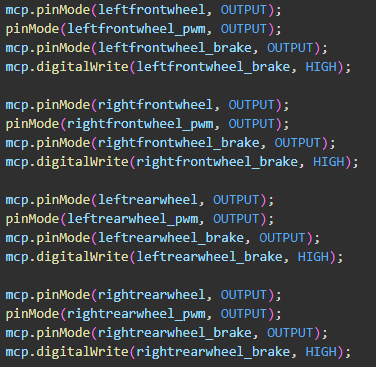
\includegraphics[scale=1.05]{Pictures/code_intialisierung_motoren}
			\captionof{figure}{Initialisierung Motoren}
			\label{fig:code_intialisierung_motoren}
			\vspace{-2pt}
			\small Quelle: eigene Abbildung
			\vspace{10pt}
		\end{minipage}	
	\subsubsection{Handling der Steuerbefehle}
	Um den Roboter zu steuern, werden die verschiedenen Steuerbefehle von der Webseite durch spezifische Funktionen bearbeitet. Die Richtungsbefehle zur Steuerung des Roboters werden mit einer Art State-Maschine beziehungsweise mit einer switch-case Struktur realisiert. Dafür wird zunächst ein enum (Enumeration) erstellt, dass die möglichen Bewegungsrichtungen des Roboters definiert und die Direction wird sofort auf „HALT“ gesetzt. Außerdem wird die Variable speed\_cb für die Geschwindigkeit initialisiert. \\[0.5cm]
	\begin{minipage}{\textwidth}
		\centering
		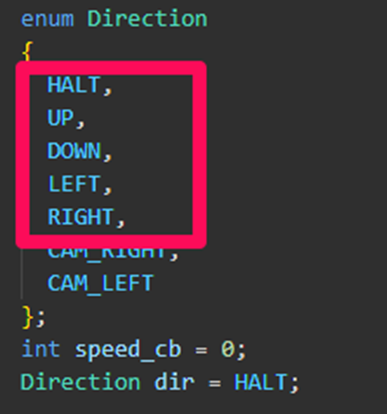
\includegraphics[scale=1.05]{Pictures/code_enum_motoren}
		\captionof{figure}{Enumeration von Bewegungsrichtungen}
		\label{fig:code_enum_motoren}
		\vspace{-2pt}
		\small Quelle: eigene Abbildung
		\vspace{10pt}
	\end{minipage}	
	\subsubsection*{Befehle zum Steuern:}
	\begin{itemize}
		\item HALT: Der Roboter bremst.
		\item UP: Bewegt den Roboter vorwärts.
		\item DOWN: Bewegt den Roboter rückwärts.
		\item LEFT: Lässt den Roboter nach links drehen.
		\item RIGHT: Lässt den Roboter nach rechts drehen.
	\end{itemize}\newpage
	\noindent
	Um die Befehle von der Webseite für die Steuerung zu benutzen, werden zunächst die erhaltenen Strings, mit einer Funktion in die vorhin definierte Richtungsvariable umgewandelt. \\[0.5cm]
	\begin{minipage}{\textwidth}
		\centering
		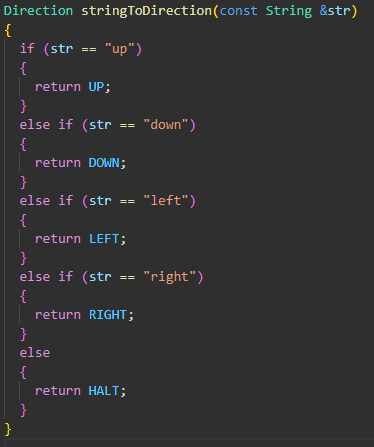
\includegraphics[scale=1.0]{Pictures/code_stringtoenum_motoren}
		\captionof{figure}{Strings zu Enum Variable umwandeln}
		\label{fig:code_stringtoenum_motoren}
		\vspace{-2pt}
		\small Quelle: eigene Abbildung
	\end{minipage}
	\subsubsection{Ansteuerung der Treiberplatinen:}
	Die Geschwindigkeit und die Richtung des Roboters werden schlussendlich in der Funktion „void navigate()“ bearbeitet. Diese Funktion wird in der „void loop()“ die ganze Zeit ausgeführt. \\[0.5cm]
	\begin{minipage}{\textwidth}
		\centering
		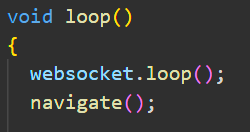
\includegraphics[scale=0.9]{Pictures/code_loop_motoren}
		\captionof{figure}{\texttt{navigate() in loop()}}
		\label{fig:code_loop_motoren}
		\vspace{-2pt}
		\small Quelle: eigene Abbildung
	\end{minipage}
	Zu Beginn werden zwei statische Variablen definiert, die dazu dienen, die zuletzt empfangene Fahrtrichtung (lastDir) und Geschwindigkeit (lastSpeed) zu speichern. Anschließend wird überprüft, ob sich entweder die Richtung oder die Geschwindigkeit im Vergleich zum vorherigen Wert geändert hat. Falls sich die Geschwindigkeit im Vergleich zum vorherigen Wert geändert hat, wird der empfangene String von der Webseite in einen Integer umgewandelt. Der Wert von „speed“ liegt im Bereich von 0–100 \% und wird in einen Wert von 0–255 skaliert, der später für die PWM-Signale verwendet wird. \\[0.5cm]
	\begin{minipage}{\textwidth}
		\centering
		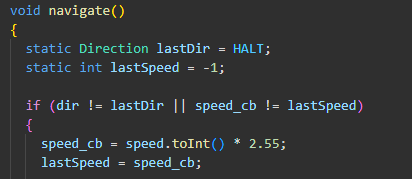
\includegraphics[scale=1.2]{Pictures/code_navigate_speed_umwandeln_motoren}
		\captionof{figure}{Überprüfung auf Änderung und Speed \\in Integer umwandeln in \texttt{navigate()}-Funktion}
		\label{fig:code_navigate_speed_umwandeln_motoren}
		\vspace{-2pt}
		\small Quelle: eigene Abbildung
		\vspace{10pt}
	\end{minipage}
	Außerdem wird die Motorbremse deaktiviert, sodass sich der Roboter überhaupt bewegt und sich steuern lässt. \\[0.5cm]
	\begin{minipage}{\textwidth}
		\centering
		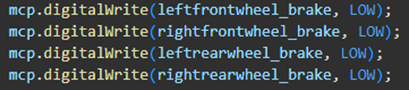
\includegraphics[scale=1.2]{Pictures/code_motorbremse_motoren}
		\captionof{figure}{Motorbremse deaktivieren in \texttt{navigate()}-Funktion}
		\label{fig:code_motorbremse_motoren}
		\vspace{-2pt}
		\small Quelle: eigene Abbildung
		\vspace{10pt}
	\end{minipage}
	Die Steuerung der Richtung des Roboters erfolgt durch eine switch-case-Struktur, die anhand der aktuellen Fahrtrichtung (dir) die entsprechende Bewegungsfunktion aufruft. Diese Steuerlogik basiert auf dem zuvor definierten enum Direction, der die verschiedenen Zustände wie UP, DOWN, LEFT, RIGHT und HALT enthält. Diese Struktur funktioniert so ähnlich wie eine Gangschaltung, sie legt nämlich nur fest in welche Richtung sich der Motor drehen soll. \\[0.5cm]
	\begin{minipage}{\textwidth}
		\centering
		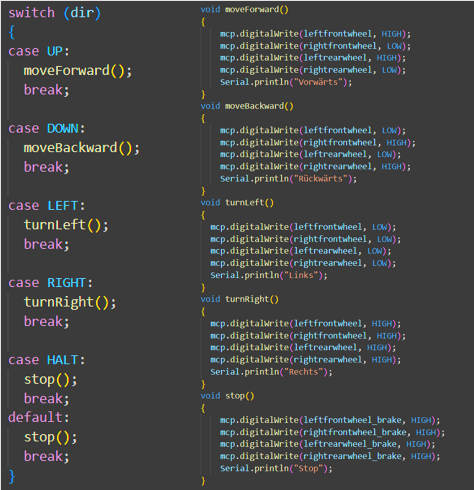
\includegraphics[scale=1.2]{Pictures/code_switch_case_motoren}
		\captionof{figure}{switch-case Struktur in \texttt{navigate()}-Funktion}
		\label{fig:code_switch_case_motoren}
		\vspace{-2pt}
		\small Quelle: eigene Abbildung
		\vspace{10pt}
	\end{minipage}
	Die Steuerung der Geschwindigkeit, wird mithilfe von PWM-Signalen umgesetzt. Zunächst wird eine statische Variable „lastPWM“ definiert, die später den zuletzt verwendeten PWM-Wert speichert. Bevor die Treiber-Platinen mit einem PWM-Signal angesteuert werden, wird überprüft, ob sich die Geschwindigkeit tatsächlich geändert hat. Falls sich „speed\_cb“ vom vorherigen Wert abweicht, werden die neuen PWM-Werte mit analogWrite() an die Motorsteuerungsplatinen gesendet, um die Geschwindigkeit der Motoren entsprechend anzupassen. \\
	\newpage 	\noindent
	Danach wird der Wert von „lastPWM“ aktualisiert, um sicherzustellen, dass die gleiche Geschwindigkeit nicht unnötig erneut gesetzt wird. Zusätzlich wird die Variable „lastDir“ aktualisiert, um die letzte Richtung zu speichern. \\[0.5cm]
	\begin{minipage}{\textwidth}
		\centering
		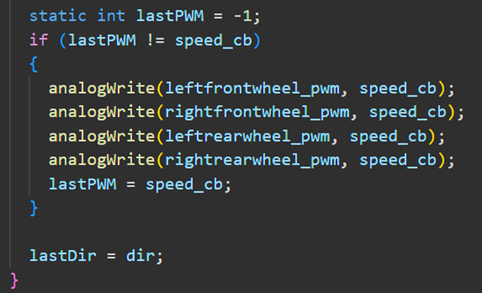
\includegraphics[scale=1.2]{Pictures/code_analogWrite_pwm_motoren}
		\captionof{figure}{PWM mit analogWrite übertragen und \\ letzte Werte speichern in \texttt{navigate()}-Funktion}
		\label{fig:code_analogWrite_pwm_motoren}
		\vspace{-2pt}
		\small Quelle: eigene Abbildung
		\vspace{10pt}
	\end{minipage}
	\newpage
	\section{Webserver} %Spari
	 
		\subsection{Grundlegende Ziele}
	In diesem Kapitel wird die geplante Website thematisiert, die die Steuerung des Lastenroboters ermöglichen soll. Zunächst werden die grundlegenden Funktionen definiert, die die Website erfüllen muss. Sobald diese Anforderungen umgesetzt sind, liegt der Fokus auf einer möglichst einfachen und benutzerfreundlichen Gestaltung des User Interfaces. Ein weiterer zentraler Aspekt ist die Darstellung spezifischer Messwerte und Daten, sodass diese über den Webserver schnell und unkompliziert zugänglich sind. \\[0.5cm]
	Für die Entwicklung der Website kommen HTML, CSS und JavaScript zum Einsatz, um sowohl die funktionalen als auch die optischen Anforderungen zu erfüllen. 
	
			\subsubsection*{Videoübertragung} 	 
	
	Die Website ermöglicht die Echtzeit-Videoübertragung des Kamerabilds der ESP32-CAM. Die Bildfrequenz und die Qualität der Videoübertragung sollte ausgeglichen sein, so dass in der Übertragung alle Objekte und ggf. Hindernisse frühzeitig erkennbar sind und noch Reaktionszeit zum Manövrieren besteht. 
	
			\subsubsection*{Steuerung}
	
	Auf der Website soll eine grafische Steuereinheit implementiert werden, mit der der Roboter gesteuert und navigiert werden kann. Diese soll dann die entsprechenden Steuerbefehle bzw. Richtungen an den ESP32 senden, wo sie dann in Steuerungsbefehle für die Motoren übersetzt werden.  
	
			\subsubsection*{Anzeigen von Daten}
	
	Auf der Website sollen bestimmte Messwerte und Daten, wie zum Beispiel Akkustand oder zurzeit aufliegende Last, die vom ESP32 durch Sensoren oder Messungen ausgewertet werden, übersichtlich und leicht zugänglich angezeigt werden. \newpage
		
		\subsection{Webserver}
		
			\subsubsection{Webserver Setup}
			
	Der Webserver wird auf einem ESP32-CAM Mikrocontroller mithilfe der Bibliothek ESPAsyncWebServer  eingerichtet. Diese Bibliothek ermöglicht einen nicht-blockierenden Betrieb, wodurch parallele Anfragen effizient verarbeitet werden können.\footnote{https://github.com/lacamera/ESPAsyncWebServer} \\[0.5cm]
	\begin{minipage}{\textwidth}
		\centering
		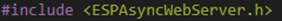
\includegraphics[scale=1]{Pictures/espasyncwebserver}
		\captionof{figure}{\texttt{ESPAsyncWebServer.h}-Bibliothek}
		\label{fig:espasyncwebserver}
		\vspace{-2pt}
		\small Quelle: eigene Abbildung
	\end{minipage} \\[0.75cm]
	\subsubsection*{Netzwerkkonfiguration}
	Die ESP32-CAM fungiert als Access Point mit folgenden Konfigurationen:
	
	\begin{itemize}
		\item SSID (Service Set Identifiert) : “Carybot” – dient zur Identifikation des drahtlosen Netwerkes
		\item Passwort: “123456789“ – dient zum Schutz des Netwerkes
		\item Lokale IP-Adresse: 192.168.4.1 – dient zum Zugriff auf die Webserver-Oberfläche
		\item Gateway-Adresse: 192.168.4.1 - ESP32-CAM fungiert als Access Point
		\item Subnetzmaske: 255.255.255.0 - ermöglicht die Kommunikation zwischen Geräten im Bereich 192.168.4.x
		\item Port: 80 - Standardport für HTTP-Dienste
	\end{itemize} 
	\begin{minipage}{\textwidth}
		\centering
		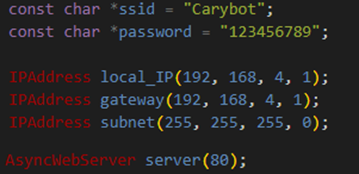
\includegraphics[scale=1]{Pictures/server-config}
		\captionof{figure}{WebServer Netzwerkkonfiguration}
		\label{fig:server-config}
		\vspace{-2pt}
		\small Quelle: eigene Abbildung
	\end{minipage} \\[0.75cm]
	In der Setup Funktion wird danach überprüft, ob der Access Point erfolgreich konfiguriert worden ist und ob er erfolgreich gestartet werden kann. Falls ein Fehler auftreten sollte, wird der Setup unterbrochen und die jeweilige Fehlermeldung in der seriellen Konsole ausgegeben. Wenn alles erfolgreich konfiguriert ist und starten kann, wird im Seriellen Monitor die IP-Adresse in der seriellen Konsole ausgegeben. Anschließend wird der Webserver gestartet. \\[0.5cm]
	\begin{minipage}{\textwidth}
		\centering
		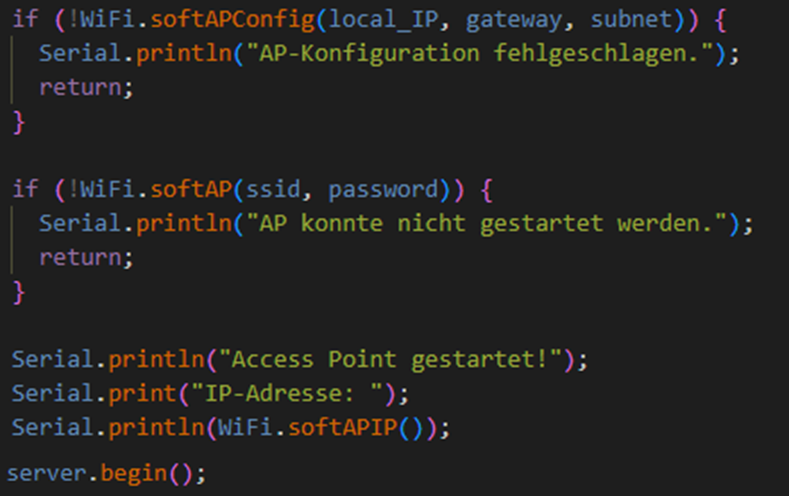
\includegraphics[scale=0.7]{Pictures/server-setup}
		\captionof{figure}{Webserver Setup}
		\label{fig:server-setup}
		\vspace{-2pt}
		\small Quelle: eigene Abbildung
	\end{minipage} \\[0.5cm]
			
			\subsubsection{SPIFFS Setup}
			
	SPIFFS (SPI Flash File System) ist ein leichtgewichtiges Dateisystem für Mikrocontroller mit SPI-Flash-Speicher. Es ermöglicht das Speichern und Verwalten von Dateien direkt im Flash-Speicher des Mikrocontrollers. SPIFFS wird in unserem Projekt benötigt, um statische Dateien für unseren Webserver (HTML-, CSS-, JavaScript Anwendungen) bereitzustellen. \\[0.5cm] 
	In unserem Code wird zuallererst einmal überprüft, ob SPIFFS beim Start der ESP32-CAM richtig initialisiert werden kann. Falls es fehlschlägt, wird eine Fehlermeldung in der seriellen Konsole ausgegeben und das Programm gestoppt. Ansonsten werden die Webserver-Endpunkte über HTTP-GET-Routen definiert, über die unsere statischen Dateien aus SPIFFS an Clients gesendet werden. \\[0.5cm] 
	“/“ ist die Default-Route des Servers. Somit wird dpad.html als Startseite angezeigt, wenn ein Client sich verbindet. \\[0.5cm] 
	“menu-icon.svg“ und “Fernlicht.svg“ werden als SVG-Bilder (Scalable Vector Graphics) an den Browser gesendet. Image/svg+xml sorgt dafür, dass der Browser die Dateien als SVG-Bilder erkennt. \\[0.5cm] 
	“mystyles.css“ wird mit text/css als CSS-Datei gesendet und dient zur Formatierung der Website. \\[0.5cm] 
	“carybot.js“ wird mit application/javascript als Javascript-Datei gesendet und verarbeitet die Eingaben von Clients auf der Website. \\[0.5cm] 
	Wenn alle Dateien erfolgreich geladen sind, wird eine Nachricht in der seriellen Konsole ausgegeben. \\
	
	\begin{center}
		\begin{minipage}[t]{0.75\textwidth}
			\includegraphics[scale=0.7]{Pictures/SPIFFS\_setup}
			\captionof{figure}{SPIFFS Initalisierung}
			\label{fig:spiffs_init}
			\vspace{-10pt}
			\begin{center}
				\par\small Quelle: eigene Abbildung
			\end{center}
		\end{minipage} \\[2cm]
	\end{center}
	Die readFile() Funktion wird benötigt, um die jeweiligen Dateien aus SPIFFS lesen zu können. Die Funktion liest eine Datei aus dem SPIFFS-Speicher und gibt den Inhalt als String zurück.\\
	
	\begin{center}
		\begin{minipage}[t]{0.75\textwidth}
			\includegraphics{Pictures/spiffs\_readfile}
			\captionof{figure}{\texttt{readfile()}-Funktion}
			\label{fig:spiffs_readfile}
			\vspace{-10pt}
			\begin{center}
				\par\small Quelle: eigene Abbildung
			\end{center}
		\end{minipage} \\[0.75cm]
	\end{center}

	
		\subsection{WebSocket Kommunikation}
		
			\subsubsection{Kommunikation Setup}	
			
	Für die Kommunikation zwischen dem Webserver und dem ESP32 wird die ArduinoJson und die ArduinoWebSockets Bibliothek benötigt. Die ArduinoJson Bibliothek wird für die Umwandlung der JSON-Steuerbefehle benötigt. Die ArduinoWebSockets Bibliothek wird für die Kommunikation über das WebSocket Protokoll benötigt. \\
	\begin{center}
		\begin{minipage}[t]{0.45\textwidth}
			\includegraphics{Pictures/kommunikation\_libraries}
			\captionof{figure}{Bibliotheken für die Kommunikation}
			\label{fig:kommunikation_libraries}
			\vspace{-10pt}
			\begin{center}
				\par\small Quelle: eigene Abbildung 
			\end{center}
		\end{minipage} \\[0.75cm]
	\end{center}
	Für die Netzwerkkonfiguration als Client werden die gleichen Parameter wie in der Access Point Konfiguration gewählt (siehe \ref{fig:server-config}), mit Ausnahmen der IP-Adresse und dem WebSocket Port. Als Lokale IP-Adresse wurde 192.168.4.3 und als Port 8080 gewählt.\\[1cm]
	In der Setup Funktion des Programmes wird überprüft, ob die IP-Konfiguration erfolgreich abgeschlossen wurde. Ansonsten kommt es zu einer Fehlermeldung und das Setup wird abgebrochen. Danach wird versucht, sich mit dem WLAN-Netzwerk zu verbinden. Wenn sich der ESP32 erfolgreich mit dem WLAN verbunden hat, wird eine Nachricht und die IP-Adresse des ESP32 in der seriellen Konsole ausgegeben. Danach wird die WebSocket Konfiguration gestartet. Es wird definiert, dass die Funktion onWebSocketEvent aufgerufen wird, wenn Events über den WebSocket registriert werden. In der loop Funktion wird ständig überprüft, ob neue Events am WebSocket registriert werden.
	\begin{center}
		\begin{minipage}[t]{0.55\textwidth}
			\includegraphics[scale=0.5]{Pictures/kommunikation\_setup}
			\captionof{figure}{Setup ESP32}
			\label{fig:kommunikation_setup}
			\vspace{-10pt}
			\begin{center}
				\par\small Quelle: eigene Abbildung 
			\end{center}
		\end{minipage} \\[0.75cm]
	\end{center}	
	
			\subsubsection{Message Handling}
			
	In der Funktion onWebSocketEvent() werden die WebSocket-Ereignisse verarbeitet. Sie wird aufgerufen, wenn sich ein WebSocket-Client verbindent, eine Nachricht sendet oder die Verbindung sich trennt.
	Der Parameter num steht für die ID des Clients, der das Event ausgelöst hat. Der Parameter type gibt die Art des WebSocket-Event an. Der Parameter payload sind die empfangenen Daten. Der Parameter length steht für die Größe des payload-Buffers. 
	In der Funktion werden die Events mit einem switch-case verarbeitet\\[5cm]
	Übersicht der WebSocket-Ereignisse:
	
	\begin{table}[h]
		\centering
		\renewcommand{\arraystretch}{1.2}
		\setlength{\tabcolsep}{8pt}
		\begin{adjustbox}{max width=\textwidth}
    	\begin{tabular}{|l|p{5cm}|p{6cm}|}

		\hline
		\textbf{Ereignistyp} & \textbf{Beschreibung} & \textbf{Verarbeitung} \\
		\hline
		WStype\_CONNECTED & Ein neuer Client verbindet sich. & Ausgabe der Client-ID \& IP-Adresse in der Konsole \\
		\hline
		WStype\_TEXT & Eine Textnachricht wird empfangen. & Übergabe an \texttt{handleWebSocketMessage()} \\
		\hline
		WStype\_BIN & Binärdaten werden empfangen. & Nachricht in der Konsole (wird nicht verarbeitet) \\
		\hline
		WStype\_DISCONNECTED & Ein Client trennt die Verbindung. & Meldung mit der Client-ID in der Konsole. \\
		\hline
	
		\end{tabular}
		\end{adjustbox}
		\caption{Übersicht der WebSocket-Ereignisse}
		\label{tab:websocket-events}
	\end{table} 
	\begin{center}
		\begin{minipage}[t]{\textwidth}
			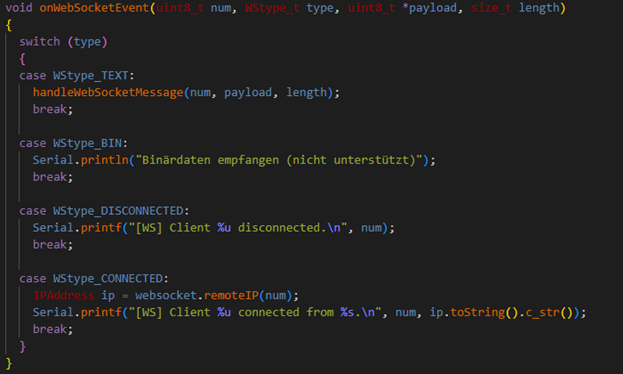
\includegraphics{Pictures/websocketevents}
			\captionof{figure}{\texttt{onWebSocketEvent()}-Funktion}
			\label{fig:onwebsocketevent}
			\vspace{-10pt}
			\begin{center}
				\par\small Quelle: eigene Abbildung 
			\end{center}
		\end{minipage} \\[0.75cm]
	\end{center}
	Die Funktion handleWebSocketMessage() verarbeitet eingehende WebSocket-Nachrichten, die als JSON-Objekte gesendet wird. Sie nimmt drei Parameter entgegen:
	\begin{enumerate}
		\item \texttt{num} - Client-ID der Websocket Verbindung
		\item \texttt{payload} - die empfangene Nachricht als Byte-Array
		\item \texttt{length} - die Länge der empfangenen Nachricht
	\end{enumerate}
	Zuerst wird das \texttt{payload}-Byte-Array in einen String konvertiert und anschließend zu Debugging-Zwecken auf der seriellen Konsole ausgegeben. Danach wird ein \texttt{StaticJsonDocument} mit einer maximalen Größe von 200 Bytes erstellt, um die empfangenen JSON-Daten zu speichern. Anschließend wird die Nachricht mit \texttt{deserializeJson()} geparst. Falls das Parsen fehlschlägt, wird die Verarbeitung abgebrochen. Je nachdem, welche Schlüssel in der JSON-Nachricht enthalten sind, werden unterschiedliche Funktionen ausgeführt. \\[0.3cm]
	Falls die JSON-Nachricht den Schlüssel \texttt{robot\_direction} enthält, wird der zugehörige Wert ausgelesen und mithilfe der Funktion \texttt{stringToDirection()} in eine interne Richtungsvariable (\texttt{dir}) umgewandelt. Zusätzlich wird der Wert für \texttt{"speed"} aus der Nachricht extrahiert und als String gespeichert. 
	\begin{center}
		\begin{minipage}[t]{0.4\textwidth}
			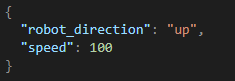
\includegraphics{Pictures/example-navigate}
			\captionof{figure}{JSON-Beispiel für Steuerung}
			\label{fig:example-speed}
			\vspace{-10pt}
			\begin{center}
				\par\small Quelle: eigene Abbildung 
			\end{center}
		\end{minipage} \\[0.3cm]
	\end{center}
	Falls die JSON-Nachricht den Schlüssel \texttt{camera\_position} enthält, wird der Wert als Ganzzahl in die Variable \texttt{camera\_pos} gespeichert. Anschließend wird die Funktion \texttt{cam\_turn()}  aufgerufen, um die Kamera entsprechend zu bewegen. 
	\begin{center}
		\begin{minipage}[t]{0.4\textwidth}
			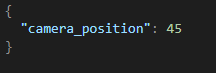
\includegraphics{Pictures/example-camera}
			\captionof{figure}{JSON-Beispiel für Kamerasteuerung}
			\label{fig:example-camera}
			\vspace{-10pt}
			\begin{center}
				\par\small Quelle: eigene Abbildung 
			\end{center}
		\end{minipage} \\[0.3cm]
	\end{center}
	Falls die JSON-Nachricht den Schlüssel \texttt{light\_status} enthält, wird der Wert der Nachricht in die boolesche Variable \texttt{light\_status}  gespeichert. Dieser Variable wird dann in die numerische Variable \texttt{light\_st} umgewandelt (1 = an, 0 = aus). Wenn \texttt{light\_st} \texttt{True} ist, wird die Funktion \texttt{lights\_on(}) aufgerufen, ansonsten wird die Funktion \texttt{lights\_off()} aufgerufen.
	\begin{center}
		\begin{minipage}[t]{0.35\textwidth}
			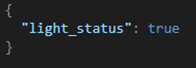
\includegraphics{Pictures/example-light}
			\captionof{figure}{JSON-Beispiel für Lichtsteuerung}
			\label{fig:example-light}
			\vspace{-10pt}
			\begin{center}
				\par\small Quelle: eigene Abbildung 
			\end{center}
		\end{minipage} 
	\end{center}
	\begin{center}
		\begin{minipage}[t]{0.85\textwidth}
			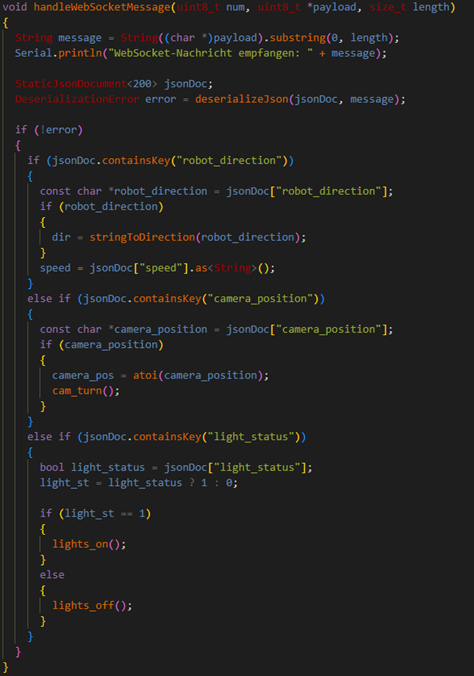
\includegraphics{Pictures/handlewebsocketmessage}
			\captionof{figure}{\texttt{handleWebSocketMessage()}-Funktion}
			\label{fig:handlewebsocketmessage}
			\vspace{-10pt}
			\begin{center}
				\par\small Quelle: eigene Abbildung 
			\end{center}
		\end{minipage} \\[0.75cm]
	\end{center} \newpage

	\subsection{Website}

		\subsubsection{Implementierung der Steuerung}
			
			\subsubsection*{Steuerkreuz}
				
	Um den Roboter überhaupt steuern zu können, wird ein Steuerkreuz implementiert. Das Steuerkreuz befindet sich mittig am rechten Bildschirmrand. Das Steuerkreuz besteht aus fünf Tasten, nämlich: Vorwarts (\texttt{UP}), (\texttt{DOWN} ), links (\texttt{LEFT}), rechts (\texttt{RIGHT}) und in der Mitte Stop (\texttt{HALT}). \\[0.5cm]
	\begin{center}
		\begin{minipage}[t]{1\textwidth}
			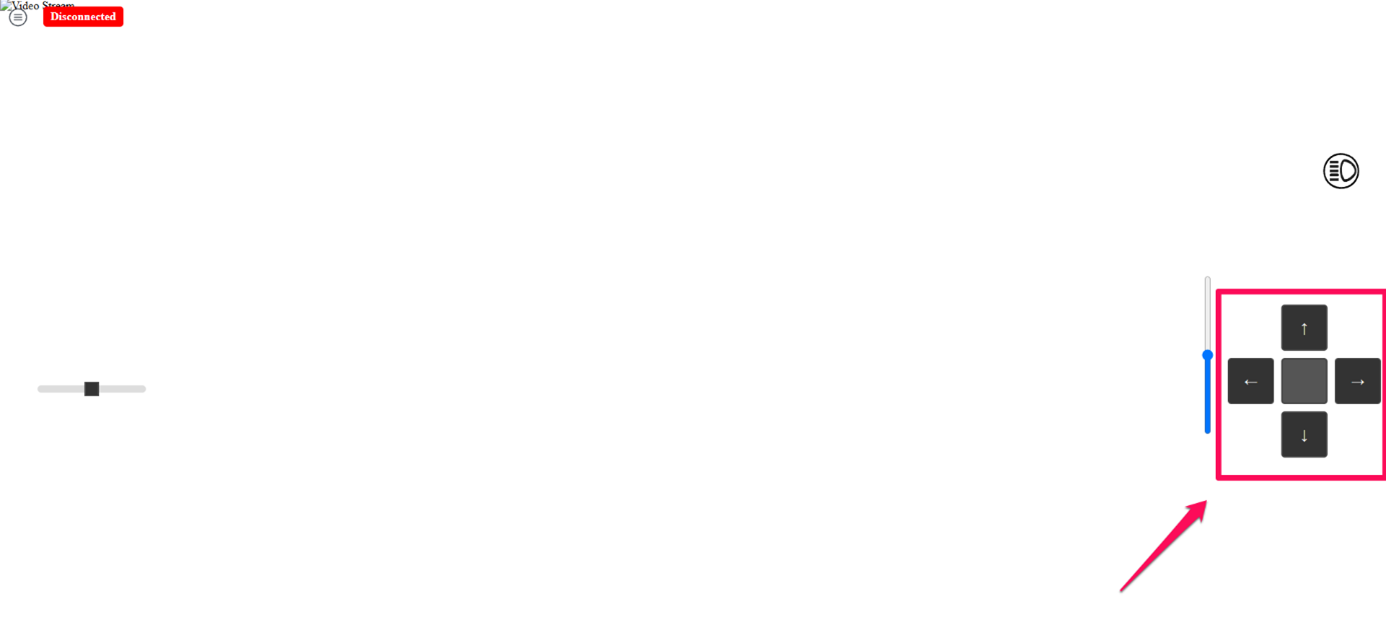
\includegraphics[scale=0.4]{Pictures/Steuerung-web}
			\captionof{figure}{Steuerkreuz auf der Website}
			\label{fig:Steuerkreuz-web}
			\vspace{-10pt}
			\begin{center}
				\par\small Quelle: eigene Abbildung 
			\end{center}
		\end{minipage} \\[0.75cm]
	\end{center}
	Im HTML-Code wird das Steuerkreuz als HTML \texttt{<div>}-Tag im body Bereich definiert. Für die Formatierung wird die CSS-Klasse \texttt{dpad-container} verwendet. Die einzelnen Richtungstasten des Steuerkreuze werden auch als HTML \texttt{<div>}-Tags definiert. Jede Taste wird mit der CSS-Klasse \texttt{button} und der jeweiligen Zusatzklasse \texttt{up/down/left/right/center} formatiert. Beim jeweiligen Tastendruck wird außerdem immer das Attribut \texttt{data-direction} mit der jeweiligen Richtung belegt.
	\begin{center}
		\begin{minipage}[t]{0.65\textwidth}
			\includegraphics[scale=0.8]{Pictures/Steuerung-html}
			\captionof{figure}{Steuerkreuz HTML-Code}
			\label{fig:Steuerkreuz-html}
			\vspace{-10pt}
			\begin{center}
				\par\small Quelle: eigene Abbildung 
			\end{center}
		\end{minipage} \\[0.75cm]
	\end{center}
	Die CSS-Klasse \texttt{dpad-container } ist das übergeordnete Element, welches die Steuerkreuztasten enthalten. Es wird als CSS Grid mit einer 3x3 Struktur definiert. Es gibt Lücken (.) an den Ecken, damit man die Form eines Steuerkreuzes erhält. Der Abstand zwischen den Tasten wird mit 10px festgelegt. Der Container hat eine feste Breite von 120px und ist vertikal so wie horizontal zentriert. \\[0.5cm]
	Die CSS-Klasse \texttt{button} sorgt für eine einheitliche Gestaltung der Tasten des Steuerkreuzes. Jede Taste hat eine Größe von 60x60px. Eine Flexbox wird verwendet, um die Tasten jeweils mittig in den einzelnen Positionen des Grids zu positionieren. Jede Taste hat einen dunkelgrauen Hintergrund, eine weiße Textfarbe, einen 2px dicken dunklen Rahmen und abgerundete Ecken. Die Optionen \texttt{-webkit-tap-highlight-color: transparent} und \texttt{user-select: none} sorgen dafür, dass auf mobilen Geräten der Text in den Tasten nicht blau markiert werden kann, damit die Steuerung nicht blockiert wird. 
	\begin{center}
		\begin{minipage}[t]{0.55\textwidth}
			\includegraphics[scale=0.9]{Pictures/Steuerung-css1}
			\captionof{figure}{CSS-Klassen \texttt{.dpad-container} und \texttt{.button}}
			\label{fig:Steuerkreuz-css1}
			\vspace{-10pt}
			\begin{center}
				\par\small Quelle: eigene Abbildung 
			\end{center}
		\end{minipage} \\[0.75cm]
	\end{center}
	Die fünf Richtungsklassen sorgen dafür, dass die Tasten des Steuerkreuzes in den zuvor definierten Grid-Bereichen zugewiesen und richtig platziert werden. Die mittlere Taste bekommt außerdem eine leicht hellere Farbe zugewiesen, um ihn optisch von den anderen abzuheben. \\[0.5cm]
	Außerdem bekommen alle Tasten einen Hover-Effekt, damit sie etwas heller werden, wenn eine Taste gedrückt wird. \\
	\begin{center}
		\begin{minipage}[t]{0.45\textwidth}
			\includegraphics{Pictures/Steuerung-css2}
			\captionof{figure}{CSS-Richtungsklassen}
			\label{fig:Steuerkreuz-css2}
			\vspace{-10pt}
			\begin{center}
				\par\small Quelle: eigene Abbildung 
			\end{center}
		\end{minipage} \\[0.75cm]
	\end{center}
	Im JavaScript-Code sorgen zwei EventListener dafür, dass die Elemente auf der Seite nicht ziehbar und verschiebbar sind und dass das Rechtsklick-Menü nicht geöffnet werden kann. Diese Maßnahmen verhindern unerwünschte Benutzerinteraktionen und sorgen für eine reibungslose Bedienung. \\[0.5cm]
	\begin{center}
		\begin{minipage}[t]{0.7\textwidth}
			\includegraphics{Pictures/Steuerung-js1}
			\captionof{figure}{EventListener für ungewünschte Aktionen}
			\label{fig:Steuerkreuz-js1}
			\vspace{-10pt}
			\begin{center}
				\par\small Quelle: eigene Abbildung 
			\end{center}
		\end{minipage} \\[0.75cm]
	\end{center}
	Vier weitere EventListener kümmern sich um die Eingabe des Steuerkreuzes. Es wird zuerst jeder \texttt{mousedown} (Linksklick) bzw. ein \texttt{touchstart} (klick auf mobile Geräte) abgefangen. Danach wird überprüft, ob das geklickte Element innerhalb eines \texttt{.button} Elements (Steuerkreuztaste) liegt. Falls ja, wird die Richtung aus dem data-direction-Attribut gelesen und an die \texttt{send()} Funktion übergeben. Wenn ein \texttt{mouseup} (Maus loslassen) oder ein \texttt{touchend} (Finger loslassen) abgefangen wird, wird die Funktion \texttt{stop()} aufgerufen. 
	\begin{center}
		\begin{minipage}[t]{0.5\textwidth}
			\includegraphics[scale=0.7]{Pictures/Steuerung-js2}
			\captionof{figure}{EventListener für Eingabe}
			\label{fig:Steuerkreuz-js2}
			\vspace{-10pt}
			\begin{center}
				\par\small Quelle: eigene Abbildung 
			\end{center}
		\end{minipage} \\[0.75cm]
	\end{center}
	Die JavaScript Funktion \texttt{send()} kümmert sich um das Senden der Steuerungsbefehle. Zuerst wird überprüft, ob die aktuelle Richtung nicht bereits die gewünschte Richtung ist. Falls ja, wird ein JSON-Objekt erstellt, welche die Richtung sowie die Geschwindigkeit enthält. Zu debug-Zwecken wird die Richtung sowie die Geschwindigkeit in der Webkonsole ausgegeben. Danach wird überprüft, ob die WebSocket-Verbindung zur ESP32-CAM offen ist. Wenn ja, wird die Nachricht auch für debug-Zwecken an die ESP32-CAM gesendet, ansonsten wird eine Fehlermeldung ausgegeben. Dasselbe geschieht für die WebSocket-Verbindung zum ESP32. Dort werden jedoch die Steuerbefehle weiterverarbeitet. \\
	\begin{center}
		\begin{minipage}[t]{0.75\textwidth}
			\includegraphics[scale=0.7]{Pictures/Steuerung-js3}
			\captionof{figure}{\texttt{send()}-Funktion}
			\label{fig:Steuerkreuz-js3}
			\vspace{-10pt}
			\begin{center}
				\par\small Quelle: eigene Abbildung 
			\end{center}
		\end{minipage} \\[0.75cm]
	\end{center}
	Die JavaScript Funktion \texttt{stop()} sorgt dafür, dass der Roboter anhält, wenn eine Taste des Steuerkreuzes losgelassen wird. Zuerst wird überprüft, ob die aktuelle Richtung nicht bereits \texttt{HALT} ist, ansonsten wird sie überschrieben. Danach wird ein Stopp-Befehl als JSON-Nachricht vorbereitet. Zu debug-Zwecken wird wieder ein halt in der Webkonsole ausgegeben. Danach wird der Stopp-Befehl wieder an die WebSocket-Verbindung zur ESP32-CAM für debug-Zwecke gesendet. Danach wird sie auch an die WebSocket-Verbindung zum ESP32 gesendet, wo dieser weiterverarbeitet wird. \\[0.5cm]
	\begin{center}
		\begin{minipage}[t]{0.75\textwidth}
			\includegraphics[scale=0.7]{Pictures/Steuerung-js4}
			\captionof{figure}{\texttt{stop()}-Funktion}
			\label{fig:Steuerkreuz-js4}
			\vspace{-10pt}
			\begin{center}
				\par\small Quelle: eigene Abbildung 
			\end{center}
		\end{minipage} \\[0.75cm]
	\end{center}
				
				\subsubsection*{Geschwindigkeitseinstellung}
			
	Um die Fortbewegungsgeschwindigkeit des Roboters kontrollieren zu können, gibt es auf der linken Seite neben dem Steuerkreuz einen vertikalen Geschwindigkeitsslider, mit der die Geschwindigkeit der Motoren gesteuert werden kann. Wenn der Slider nach oben gezogen wird, beschleunigt der Roboter, wenn der Slider nach unten gezogen wird, wird die Geschwindigkeit verlangsamt. \\[0.5cm]
	\begin{center}
		\begin{minipage}[t]{1\textwidth}
			\includegraphics[scale=0.9]{Pictures/speed-web}
			\captionof{figure}{Geschwindigkeitssteuerung auf der Website}
			\label{fig:speed-web}
			\vspace{-10pt}
			\begin{center}
				\par\small Quelle: eigene Abbildung 
			\end{center}
		\end{minipage} \\[0.75cm]
	\end{center}
	Im HTML-Code wird mit der CSS-Klasse \texttt{slider-container} ein Bereich im Hauptbereich definiert. Der Slider wird als HTML \texttt{<input>}-Tag mit dem type \texttt{range} von 0 bis 100 definiert. Für das Design wird die CSS-Klasse \texttt{slider} verwendet und beim Verschieben des Sliders wird die JavaScript Funktion \texttt{speed\_change()} mit der aktuellen Position des Sliders aufgerufen. \\
	\begin{center}
		\begin{minipage}[t]{1\textwidth}
			\includegraphics[scale=0.9]{Pictures/speed-html}
			\captionof{figure}{Geschwindigkeitssteuerung HTML-Code}
			\label{fig:speed-html}
			\vspace{-10pt}
			\begin{center}
				\par\small Quelle: eigene Abbildung 
			\end{center}
		\end{minipage} \\[0.75cm]
	\end{center}
	In der CSS-Klasse \texttt{slider-container} wird ein Bereich mit der Größe 50x220 Pixel definiert, in dem der Slider angezeigt werden soll. In \texttt{slider} wird definiert, dass der Slider vertikal und nicht horizontal angezeigt wird. Außerdem wird die Richtung auf \texttt{Right to Left} gesetzt, damit beim Hochschieben des Sliders die aktuelle Position erhöht und beim Runterschieben vermindert wird. \\
	\begin{center}
		\begin{minipage}[t]{0.45\textwidth}
			\includegraphics{Pictures/speed-css}
			\captionof{figure}{CSS-Klassen für die Geschwindigkeitssteuerung}
			\label{fig:speed-css}
			\vspace{-10pt}
			\begin{center}
				\par\small Quelle: eigene Abbildung 
			\end{center}
		\end{minipage} \\[1.5cm]
	\end{center}
	Im JavaScript-Code wird die aktuelle Position des Sliders in die eigene Variable \texttt{speed} gespeichert. Die Geschwindigkeit wird immer bei einem Steuerbefehl des Steuerkreuzes mitübertragen. (siehe Steuerkreuz  \ref{fig:Steuerkreuz-js4})
	\begin{center}
		\begin{minipage}[t]{0.55\textwidth}
			\includegraphics{Pictures/speed-js}
			\captionof{figure}{\texttt{speed-change()}-Funktion}
			\label{fig:speed-js}
			\vspace{-10pt}
			\begin{center}
				\par\small Quelle: eigene Abbildung 
			\end{center}
		\end{minipage} \\[0.75cm]
	\end{center}
				
				\subsubsection*{Kamerasteuerung}
				
	Um mit der Videoübertragung besser Objekte und Hindernisse zu erkennen, ist die Kamera leicht schwenkbar. Um nun die Kamera auf unserer Website bewegen zu können, gibt es auf der linken Seite einen horizontalen Slider, mit der die Kamera ein Stück links und rechts geschwenkt werden kann. \\[0.5cm]
	\begin{center}
		\begin{minipage}[t]{1\textwidth}
			\includegraphics[scale=0.9]{Pictures/kamera-web}
			\captionof{figure}{Kamerasteuerung auf der Website}
			\label{fig:kamera-web}
			\vspace{-10pt}
			\begin{center}
				\par\small Quelle: eigene Abbildung 
			\end{center}
		\end{minipage} \\[0.75cm]
	\end{center}
	Im HTML-Code wird ein mit der CSS-Klasse \texttt{camera-container} ein Bereich im Hauptbereich definiert. Der Slider wird als HTML \texttt{<input>}-Tag mit dem type \texttt{range} von 0 bis 180 definiert. Für das Design wird die CSS-Klasse \texttt{cam\_slider} verwendet und beim Verschieben des Sliders wird die JavaScript Funktion \texttt{camera\_change()} mit der aktuellen Position des Sliders aufgerufen. \\[0.5cm]
	\begin{center}
		\begin{minipage}[t]{1\textwidth}
			\includegraphics{Pictures/kamera-html}
			\captionof{figure}{Kamerasteuerung HTML-Code}
			\label{fig:kamera-html}
			\vspace{-10pt}
			\begin{center}
				\par\small Quelle: eigene Abbildung 
			\end{center}
		\end{minipage} \\[0.75cm]
	\end{center}
	In der CSS-Klasse \texttt{camera-container} wird ein Bereich erstellt, in dem der Slider angezeigt werden soll.  In \texttt{cam\_slider} wird die Slidespur mit einer Breite von 150 Pixel und einer Höhe von 10 Pixel definiert. Der Hintergrund ist hellgrau und die Ecken werden leicht abgerundet.  In \texttt{webkit-slider-thumb} wird der Sliderknopf mit 20x20 Pixel definiert. Der Hintergrund ist dunkelgrau mit einem 2px breiten, dunkleren Rand. \\
	\begin{center}
		\begin{minipage}[t]{0.5\textwidth}
			\includegraphics{Pictures/kamera-css}
			\captionof{figure}{CSS-Klassen für die Kamerasteuerung}
			\label{fig:kamera-css}
			\vspace{-10pt}
			\begin{center}
				\par\small Quelle: eigene Abbildung 
			\end{center}
		\end{minipage} \\[2cm]
	\end{center}
	Im JavaScript-Code wird die aktuelle Position des Sliders verarbeitet. Dazu wird die Position in eine JSON-Nachricht gespeichert. Zu debug-Zwecken wird die Position noch in der Website Konsole ausgegeben. Wenn der WebSocket Verbindung zum ESP32 offen ist, wird die aktuelle Position übermittelt. \\
	\begin{center}
		\begin{minipage}[t]{0.75\textwidth}
			\includegraphics{Pictures/kamera-js}
			\captionof{figure}{\texttt{camera-change()}-Funktion}
			\label{fig:kamera-js}
			\vspace{-10pt}
			\begin{center}
				\par\small Quelle: eigene Abbildung 
			\end{center}
		\end{minipage} \\[0.5cm]
	\end{center}	
				\subsubsection*{Fernlicht}
				
	Die Funktion des Fernlichts dient bei unserem Roboter zur Beleuchtung bei schlechter Sicht bzw. Dunkelheit. Wenn eingeschalten, leuchtet auf der Vorder- sowie auf der Hinterseite des Roboters ein Scheinwerfer die Umgebung aus. \\[0.5cm]
	Um das Fernlicht auf unserer Website ein- bzw. auszuschalten gibt es ein eigenes Fernlicht-Icon rechts über dem Steuerkreuz. Im ausgeschalteten Zustand ist das Icon ausgegraut. Im aktiven Zustand ist das Scheinwerfer Symbol im Icon blau und das Icon hat einen blassgrünen Hintergrund. \\[0.5cm]
	\begin{center}
		\begin{minipage}[t]{0.65\textwidth}
			\includegraphics[scale=0.6]{Pictures/fernlicht-web}
			\captionof{figure}{Fernlicht-Icon auf der Website}
			\label{fig:fernlicht-web}
			\vspace{-10pt}
			\begin{center}
				\par\small Quelle: eigene Abbildung 
			\end{center}
		\end{minipage} \\[0.75cm]
	\end{center}
	Im HTML-Code wird das Icon als HTML \texttt{<img>}-Tag eingefügt. Als Quelle wird die im SPIFFS hochgeladene \texttt{Fernlicht.svg} Grafik verwendet. Für das Design wird die CSS-Klasse \texttt{fernlicht-icon} verwendet und beim \texttt{onclick} Event wird die JavaScript Funktion \texttt{togglelight()} aufgerufen. \\
	\begin{center}
		\begin{minipage}[t]{1\textwidth}
			\includegraphics[scale=0.9]{Pictures/fernlicht-html}
			\captionof{figure}{HTML-Code für Fernlicht}
			\label{fig:fernlicht-html}
			\vspace{-10pt}
			\begin{center}
				\par\small Quelle: eigene Abbildung 
			\end{center}
		\end{minipage} \\[0.75cm]
	\end{center}
	In der CSS-Klasse \texttt{fernlicht-icon} wird das Icon 20\% vom oberen Rand und 2\% von rechten Rand mit einer Größe von 50x50 Pixel positioniert. Es wird auf der 2 z-Ebene angezeigt und der nicht sichtbare Hintergrund wird transparent angezeigt. Beim Ändern der Farbe wird eine sanfte Animation über 0,3 Sekunden angezeigt. \\[0.5cm]
	Die \texttt{grayscale} Klasse wandelt das Icon in die ausgegraute Darstellung um, um anzuzeigen, dass das Fernlicht deaktiviert ist.
	Die \texttt{active-light} Klasse ändert die Hintergrundfarbe zu einem transparenten grünen Ton, um anzuzeigen, dass das Fernlicht aktiv ist. \\[0.5cm]
	\begin{center}
		\begin{minipage}[t]{0.65\textwidth}
			\includegraphics{Pictures/fernlicht-css}
			\captionof{figure}{CSS-Klassen für das Fernlicht}
			\label{fig:fernlicht-css}
			\vspace{-10pt}
			\begin{center}
				\par\small Quelle: eigene Abbildung 
			\end{center}
		\end{minipage} \\[0.75cm]
	\end{center}
	Im JavaScript Code wird bei jedem \texttt{onclick} Event die Variable \texttt{light} getoggled. Wenn die Variable \texttt{light} true ist, wird die CSS-Klasse \texttt{active-light} angewendet, ansonsten die CSS-Klasse \texttt{grayscale}. Anschließend wird eine JSON-Nachricht mit dem aktuellen Zustand der \texttt{light} Variable erstellt. Wenn die WebSocket Verbindung zum zum ESP32 offen ist, wird die JSON-Nachricht versendet, ansonsten wird eine Fehlermeldung ausgegeben. \\[0.5cm]
	\begin{center}
		\begin{minipage}[t]{0.95\textwidth}
			\includegraphics[scale=0.9]{Pictures/fernlicht-js}
			\captionof{figure}{\texttt{togglelight()}-Funktion}
			\label{fig:fernlicht-js}
			\vspace{-10pt}
			\begin{center}
				\par\small Quelle: eigene Abbildung 
			\end{center}
		\end{minipage} \\[0.75cm]
	\end{center}
			
			\subsubsection{Anzeige von Sensordaten und Verbindungsstatus}
			
				\subsubsection*{Sensordaten}	
			
	In der linken oberen Ecke der Website befindet sich das Menü-icon. Ein Klick darauf ruft die Sidebar für die Daten auf. Die Sidebar klappt sich am linken Bildschirmrand auf. Darin kann ist der aktuelle Akkustand sowie das aktuelle aufliegende Gewicht auslesbar. Um das Menü wieder schließen zu können, ist ein erneuter Klick auf das Icon erforderlich und die Sidebar wird wieder zugeklappt. \\[0.5cm]	
	\begin{center}
		\begin{minipage}[t]{1\textwidth}
			\includegraphics[scale=0.4]{Pictures/menu-web1}
			\captionof{figure}{Menü-Icon auf der Website}
			\label{fig:menu-web}
			\vspace{-10pt}
			\begin{center}
				\par\small Quelle: eigene Abbildung 
			\end{center}
		\end{minipage} \\[0.75cm]
	\end{center}
	\begin{center}
		\begin{minipage}[t]{1\textwidth}
			\includegraphics[scale=0.9]{Pictures/sensordaten-web}
			\captionof{figure}{Sidebar mit Sensordaten}
			\label{fig:sidebar}
			\vspace{-10pt}
			\begin{center}
				\par\small Quelle: eigene Abbildung 
			\end{center}
		\end{minipage} \\[0.75cm]
	\end{center}
	Im HTML-Code wird im Body-Bereich wird das Icon als HTML \texttt{<img>}-Tag eingefügt. Als Quelle wird die im SPIFFS hochgeladene Grafik \texttt{menu-icon.svg} Grafik verwendet. Für das Design wird die CSS-Klasse \texttt{menu-icon} verwendet und beim onclick Event wird die JavaScript Funktion \texttt{togglemenu()} aufgerufen. \\[0.5cm]
	Im HTML \texttt{<div>}-Tag werden die einzelnen Daten festgelegt und mir der CSS-Klasse \texttt{mymenu} formatiert. Das Gewicht und der Akkustand werden als HTML \texttt{<p>}-Tag angezeigt und mit der CSS-Klasse \texttt{daten} formatiert. \\
	\begin{center}
		\begin{minipage}[t]{1\textwidth}
			\includegraphics{Pictures/sensordaten-html}
			\captionof{figure}{Sensordaten HTML-Code}
			\label{fig:sensordaten-html}
			\vspace{-10pt}
			\begin{center}
				\par\small Quelle: eigene Abbildung 
			\end{center}
		\end{minipage} \\[0.75cm]
	\end{center}
	In der CSS-Klasse \texttt{mymenu} wird die sidebar formatiert. Das Menü ist fixiert und nimmt 100\% der Höhe ein. Die Anfängliche Höhe ist 0, da es versteckt bzw. eingeklappt ist. Die Hintergrundfarbe ist schwarz und es befindet sich auf der z-Ebene 1 um den Hauptinhalt überdecken zu können. Beim Ein- und Ausblenden dauert 0.5 Sekunden, um einen sanften Übergang zu ermöglichen. \\[0.5cm]
	Der Hauptinhalt \texttt{\#main} hat eine Animation, damit er beim Öffnen des Menüs nach rechts verschoben werden kann. \\[0.5cm]
	Falls der Bildschirm kleiner als 450px Höhe hat, werden die Abstände der angezeigten Daten verkleinert. Das dient dazu, um besonders auf Handys die Ansicht zu optimieren. \\[0.5cm]
	Die CSS-Klasse \texttt{menu-icon} positioniert das Icon in der linken oberen Ecke mit einer 30x30px Format. \texttt{Cursor: pointer} sorgt dafür, dass das Icon anklickbar ist. \\[0.5cm]
	\begin{center}
		\begin{minipage}[t]{0.6\textwidth}
			\includegraphics[scale=0.7]{Pictures/sensordaten-css}
			\captionof{figure}{CSS-Klassen für das Menü}
			\label{fig:sensordaten-css}
			\vspace{-10pt}
			\begin{center}
				\par\small Quelle: eigene Abbildung 
			\end{center}
		\end{minipage} \\[0.75cm]
	\end{center}
	Die CSS-Klasse \texttt{daten} formatiert die einzelnen Daten im Menü. Sie werden in der Schriftart Arial, Helvetica oder sans-serif angezeigt und in der Farbe Weiß, mit der Schriftgröße 1.2em (20\% größer) mittig angezeigt. \\[0.5cm]
	\begin{center}
		\begin{minipage}[t]{0.85\textwidth}
			\includegraphics[scale=0.9]{Pictures/daten-css}
			\captionof{figure}{CSS-Klasse \texttt{.daten}}
			\label{fig:sensordaten-daten}
			\vspace{-10pt}
			\begin{center}
				\par\small Quelle: eigene Abbildung 
			\end{center}
		\end{minipage} \\[0.75cm]
	\end{center}
	In der JavaScript Funktion \texttt{connectWebSocket\_carybot()} wird im \texttt{onmessage()}-event die übertragenen Daten verarbeitet. Für debug-Zwecken werden die angekommen Daten in der WebKonsole ausgegeben. Danach werden die JSON-Nachrichten extrahiert. Wenn die Nachricht den Akkustand beinhaltet, wird dieser im HTML \texttt{<p>}-Tag mit der id \texttt{Akkustand} im Menü angezeigt. Wenn die Nachricht das Gewicht beinhaltet, wird dieses im HTML \texttt{<p>}-Tag mit der id \texttt{Gewicht} im Menü angezeigt. Falls beim Umwandeln ein Fehler auftreten sollte, wird dieser in der Webkonsole ausgegeben. \\
	\begin{center}
		\begin{minipage}[t]{1\textwidth}
			\includegraphics[scale=0.8]{Pictures/sensordaten-js}
			\captionof{figure}{JavaScript-Verarbeitung der Sensordaten}
			\label{fig:sensordaten-js}
			\vspace{-10pt}
			\begin{center}
				\par\small Quelle: eigene Abbildung 
			\end{center}
		\end{minipage} \\[0.75cm]
	\end{center}
	
				\subsubsection*{Verbindungsstatus}
	
	In der WebSocket Status-Box wird der aktuelle Verbindungszustand zum ESP32 angezeigt. Wenn keine Verbindung vorhanden ist, ist die Box rot. Wenn die Verbindung erfolgt, wird die Box grün. 
\begin{figure}
	\begin{minipage}{1\textwidth}
		\centering
		\includegraphics[scale=0.4]{Pictures/status-web}
		\caption{Statusbox auf der Website}
		\label{fig:status-web}
		{\small Quelle: eigene Abbildung}
	\end{minipage}
	
	\vspace{1.5cm} % Abstand zwischen den Bildern
	
	\begin{minipage}{0.3\linewidth}
		\centering
		\includegraphics{Pictures/status-green}
		\caption{Statusbox: Verbunden}
		\label{fig:status-green}
	\end{minipage}
	\hspace{0.1\linewidth}
	\begin{minipage}{0.3\linewidth}
		\centering
		\includegraphics{Pictures/status-red}
		\caption{Statusbox: Verbindung getrennt}
		\label{fig:status-red}
	\end{minipage}
\end{figure} \newpage 
Im HTML-Code wird die Status-Box als HTML \texttt{<span>}-Tag definiert. Für das Design wird die CSS-Klasse \texttt{status-box} kombiniert je nach Verbindungsstatus mit der Klasse \texttt{connected} oder \texttt{disconnected}. 
	\begin{center}
		\begin{minipage}[t]{1\textwidth}
			\includegraphics{Pictures/status-html}
			\captionof{figure}{Statusbox HTML-Code}
			\label{fig:status-html}
			\vspace{-10pt}
			\begin{center}
				\par\small Quelle: eigene Abbildung 
			\end{center}
		\end{minipage} \\[0.75cm]
	\end{center}
	In der CSS-Klasse \texttt{status-box} wird die grundlegende Box am linken oberen Bildschirmrand positioniert. Die Box liegt auf der zweiten z-Ebene. Die Schrift wird weiß definiert und wird fett dargestellt. Wenn eine Verbindung hergestellt wurde, wird der Hintergrund auf grün festgelegt (\texttt{status-box.connected}), ansonsten ist der Hintergrund rot (\texttt{status-box.disconnected}). \\[0.5cm]
	\begin{center}
		\begin{minipage}[t]{0.45\textwidth}
			\includegraphics{Pictures/status-css}
			\captionof{figure}{CSS-Klassen für die Statusbox}
			\label{fig:status-css}
			\vspace{-10pt}
			\begin{center}
				\par\small Quelle: eigene Abbildung 
			\end{center}
		\end{minipage} \\[0.75cm]
	\end{center}
	Im JavaScript-Code werden die \texttt{onopen()} und \texttt{onclose()} Events der WebSocket Verbindung gehandelt. Bei einem Verbindungsaufbau (\texttt{onopen()}) wird die Status-Box grün und der Text wechselt zu \texttt{Connected}. Außerdem wird eine Nachricht für Debug-Zwecke ausgegeben. Bei einem Verbindungsabbruch wird die Status-Box wieder rot und der Text wechselt zu \texttt{Disconnected}. Es wird automatisch alle 5 Sekunden ein neuer Versuch zur Verbindungsaufbau gestartet.
	\begin{center}
		\begin{minipage}[t]{0.95\textwidth}
			\includegraphics[scale=0.9]{Pictures/status-js}
			\captionof{figure}{JavaScript Funktionen für den Verbindungsstatus}
			\label{fig:status-js}
			\vspace{-10pt}
			\begin{center}
				\par\small Quelle: eigene Abbildung 
			\end{center}
		\end{minipage} \\[0.75cm]
	\end{center}
			
		\subsection{Herausforderungen und Optimierungen}
		
			\subsubsection{Probleme bei der WebSocket Kommunikation}
			
			\subsubsection{Latenz- und Performance Optimierungen}
			
							\subsubsection*{Kameraoptimierungen}
	Als Bildformat wird JPEG verwendet, um Speicherplatz zu sparen. Alternativ wäre RGB565 oder YUV422 möglich, jedoch benötigen diese aufgrund fehlender Kompression mehr Speicher und verlängern die Übertragungsdauer. \\[0.5cm]
	Für die Bildauflösung wird QVGA (320x240 Pixel) definiert. Alternativ wären noch VGA (640x480), SVGA (800x600) oder UXGA (1600x1200) möglich, jedoch benötigen diese mehr Speicher und mehr Bandbreite und verlängern dadurch die Übertragungsdauer.\\[0.5cm]
	Den Wert für die Bildqualität kann von 0 (= beste Qualität) bis 63 (= schlechteste Qualität) definiert werden. Wir definierten die Bildqualität mit 12, was ein guter Kompromiss zwischen Qualität und Speicherverbrauch ist.\\[0.5cm]
	Wir wählten für die Anzahl der Framebuffer 3. Die Anzahl sagt aus, wie viele Bilder gleichzeitig gespeichert werden können. Mehr Framebuffer erhöhen die Bildrate, benötigen jedoch mehr RAM. (siehe Kamera-Initialisierung \ref{fig:Kamera-Initialisierung})\\[0.5cm]
					
		\subsection{(Fazit und Ausblick)}
		
			\subsubsection{(Mögliche Erweiterungen und Verbesserungen)}
	\newpage
	\section{Gehäuse}
	
		\subsection{Planung und Design} %Felix
		
		Das Gehäuse des Lastenroboters wurde entwickelt, um die Sicherheit und Stabilität beim Transport von schweren Lasten zu gewährleisten. Dabei lag der Fokus auf einer stabilen Bauweise, damit der Lastenroboter ein Gewicht von zirka 25 Kilo aushaltet. 
		
			\subsubsection*{Wichtigsten Aspekte bei der Planung: }
		
		\begin{enumerate}
			\item Stabilität: Das Gehäuse muss das Eigengewicht des Roboters aber auch das Gewicht der Last aushalten.
			\item Größe: Bei der Größe ist es wichtig darauf zu achten das alle Komponenten sich sehr gut im Gehäuse ausgehen.
			\item Fahrverhalten: Durch die Verwendung von vier Räder, die jeweils über einen Motor angetrieben werden, soll eine gute Manövrierfähigkeit erreicht werden.
			\item Integration der Elektronik: Alle Komponenten müssen sicher im Gehäuse untergebracht werden.
			\item Gewichtsmessung: Die Wägezelle muss in das Gehäuse integriert werden, um eine präzise Messung zu ermöglichen.
			\item Wartungsfreundlichkeit: Bauteile sollten leicht zugänglich sein, um Reparaturen oder Anpassungen durchführen zu können.			
		\end{enumerate}
		
			\subsubsection*{Mechanische Konstruktion}
			
		Nach der Planung der wichtigsten Aspekte wurden zwei 3D-Modelle des Lastenroboters in Fusion 360 entworfen.
		
		\newpage
		
			\subsubsection*{Erstes Modell} 
			
			\vspace{20pt}
			
			\begin{center} 
				\begin{minipage}[t]{0.7\textwidth}
					\includegraphics{Pictures/modell-1}
					\captionof{figure}{Erstes Modell}
					\label{fig:Modell-1}
					\vspace{-10pt}
					\begin{center}
						\par\small Quelle: eigene Abbildung 
					\end{center}
				\end{minipage} \\[1cm]
			\end{center}
		Das erste Modell des Lastenroboters diente hauptsächlich als Prototyp. Es wurden keine genauen Maße beachtet, sondern dient als grobe Vorstellung wie der Lastenroboter aussehen könnte. Wichtig dabei war es die grundlegenden Komponenten wie Motoren, Räder und Wägezelle zu skizieren, um die allgemeine Funktionalität sicherzustellen. \\[0.5cm]
		In diesem frühen Entwicklungsstadium lag der Fokus auf der Mechanik und der Stabilität des Designs. Das erste Modell war sehr wichtig, um Schwachstellen und Optimierungsmöglichkeiten zu identifizieren und half dabei, das zweite Modell präzise und durchdacht zu planen.
		
		\newpage
		
		\subsubsection*{Zweites Modell}	
		
		\begin{center} 
			\begin{minipage}[t]{0.7\textwidth}
				\includegraphics{Pictures/modell-2}
				\captionof{figure}{Zweites Modell}
				\label{fig:Modell-2}
				\vspace{-10pt}
				\begin{center}
					\par\small Quelle: eigene Abbildung 
				\end{center}
			\end{minipage} \\[0.75cm]
		\end{center}
		Anhand der Erkenntnisse aus dem ersten Modell wurde das zweite Modell entwickelt, das als fertiges Modell für den Bau des Lastenroboters dient. In dieser Version wurden exakte Maße festgelegt und die genaue Position der Komponenten wie Räder, Motoren, Kamera und Wägezelle festgelegt. \\[0.5cm]
		Das Wichtigste beim Entwickeln ist die Größe des Gehäuses. Das Gehäuse basiert auf einem rechteckigen Stahlrahmen. Dieser Rahmen ist wichtig, weil er die Grundstruktur und Stabilität gewährleistet. Der rechteckige Rahmen des Lastenroboters hat eine Höhe von 220mm, eine breite von 400mm und eine Länge von 560mm. Die Vierkantstahlrohre haben eine Größe von 30mm mal 40mm.
		\begin{center} 
			\begin{minipage}[t]{0.7\textwidth}
				\includegraphics[scale=0.7]{Pictures/Rahmen}
				\captionof{figure}{Rahmen}
				\label{fig:Rahmen}
				\vspace{-10pt}
				\begin{center}
					\par\small Quelle: eigene Abbildung 
				\end{center}
			\end{minipage} \\[0.75cm]
		\end{center}
		Im nächsten Schritt wurde Halterung für die Elektronik Komponenten entwickelt. Dabei handelt es sich um eine Platte, die auf der Unterseite mit zwei Querstreben verstärkt wird. Die Größe der Platte beträgt 34mm mal 50mm und hat eine Materialstärke von 5mm. Die Querstreben haben eine Länge von 50mm, sind 25mm hoch und 25mm breit. \\
		\begin{figure}[h]
			\begin{minipage}{0.3\linewidth}
				\centering
				\includegraphics{Pictures/Halterung-1}
				\caption{Halterung 1}
				\label{fig:Halterung}
				\small Quelle: eigene Abbildung
			\end{minipage}
			\hspace{0.25\linewidth}
			\begin{minipage}{0.3\linewidth}
				\centering
				\includegraphics{Pictures/Halterung-2}
				\caption{Halterung 2}
				\label{fig:Halterung}
				\small Quelle: eigene Abbildung
			\end{minipage}
		\end{figure} \\
		Danach wurde die Halterung für die Motoren entwickelt. Dabei ist zu beachten, dass sich die Motoren während des Betriebs weder verdrehen noch verrutschen. Dies ist entscheidend, da die Motoren ein hohes Drehmoment erzeugen, das ohne eine stabile Befestigung zu Instabilitäten führen könnte. Die Motoren sind auf einer Querstange befestigt damit sie sich nicht mehr verdrehen können. Die Querstangen haben eine Länge von 50mm und sind 15mm hoch und 20mm breit. Zusätzlich sind die Motoren auch mit einer Schelle am Boden fixiert, um ungewolltes verrutschen zu vermeiden. \\
		\begin{center} 
			\begin{minipage}[t]{0.7\textwidth}
				\includegraphics{Pictures/Halterung-Motoren}
				\captionof{figure}{Motorenhalterung}
				\label{fig:Motorenhalterung}
				\vspace{-10pt}
				\begin{center}
					\par\small Quelle: eigene Abbildung 
				\end{center}
			\end{minipage} \\[2cm]
		\end{center}
		Nach dem die Halterung für die Motoren entwickelt wurde, erfolgt die Auswahl und Befestigung der Reifen. Die reifen spielen eine entscheidende Rolle für das Fahrverhalten. \\[0.5cm]
		Die Räder bestehen aus Gummi für einen gute Bodenhaftung. Jedes der vier Reifen ist direkt an der Motorachse befestigt. Die Motorachse hat einen Durchmesser von 16mm. Die Motorachse verfügt über ein M8-Gewinde, das für die Befestigung der Räder verwendet wird. Die Räder werden mit einer M8-Schraube in die Motorachse geschraubt.\\[0.5cm]
		Wichtig bei der Entwicklung war die Radgröße damit das Gehäuse genug Bodenabstand hat. Es wurden Reifen gewählt mit einem Durchmesser von 260mm und einer Breite von 85mm.\\
		\begin{center} 
			\begin{minipage}[t]{0.7\textwidth}
				\includegraphics{Pictures/Räder}
				\captionof{figure}{Räder}
				\label{fig:Räder}
				\vspace{-10pt}
				\begin{center}
					\par\small Quelle: eigene Abbildung 
				\end{center}
			\end{minipage} \\[0.75cm]
		\end{center}
		Ein weiterer großer Punkt bei der Planung war die Gewichtsmessung. Die Gewichtsmessung erfolgt über vier Wägezellen die in einem Rechteck auf einer Platte angeordnet sind. Auf die Wägezellen wird eine Platte montiert, auf die die Last gestellt wird.
		\begin{center} 
			\begin{minipage}[t]{0.4\textwidth}
				\includegraphics{Pictures/Wägezellen}
				\captionof{figure}{Wägezellen}
				\label{fig:Wägezellen}
				\vspace{-10pt}
				\begin{center}
					\par\small Quelle: eigene Abbildung 
				\end{center}
			\end{minipage} \\[0.75cm]
		\end{center}
		Damit die Wägezellen sicher fixiert sind und nicht verrutschen, werden sie in einer 3D-gedruckten Halterung befestigt. Die Halterung hat eine Einkerbung, die genau für die Wägezelle abgestimmt ist, damit die Wägezelle nicht mehr verrutschen kann. Es gibt zusätzlich eine Einkerbung für die Leitungen, damit diese nicht beschädigt werden. Am Rand der Halterung sind zwei Löcher damit die Halterung auf der Platte angeschraubt werden kann. 
		\begin{center} 
			\begin{minipage}[t]{0.6\textwidth}
				\includegraphics{Pictures/Halterung-wägezellen}
				\captionof{figure}{Wägezellenhalterung}
				\label{fig:Wägezellenhalterung}
				\vspace{-10pt}
				\begin{center}
					\par\small Quelle: eigene Abbildung 
				\end{center}
			\end{minipage} \\[0.75cm]
		\end{center}
		Im letzten Schritt des Designs wurden zwei Platten an der Vorderseite und Rückseite des Lastenroboters angebracht. Die hintere Platte dient für die Befestigung des An/Aus Schalters und des Ladeanschlusses für den Lastenroboter. Auf der vorderen Platte soll die Kamera montiert werden.
		\begin{center} 
			\begin{minipage}[t]{0.6\textwidth}
				\includegraphics{Pictures/modell-fertig}
				\captionof{figure}{modell-fertig}
				\label{fig:modell-fertig}
				\vspace{-10pt}
				\begin{center}
					\par\small Quelle: eigene Abbildung 
				\end{center}
			\end{minipage} \\[0.75cm]
		\end{center} 
	
		\subsubsection*{Materialwahl für das Gehäuse}
		Für das Gehäuse wurde Stahl als Hauptmaterial gewählt, weil es sehr robust und widerstandsfähig gegenüber äußeren Einflüssen ist. Ein weiter Grund, warum Stahl als Hauptmaterial verwendet wurde, ist die einfache Verarbeitung. Stahl kann man gut Schweißen aber auch verschrauben.
		
		\subsection{Realisierung} %Felix
		Nach der abgeschlossenen Planungsphase begann die schrittweise Umsetzung des Baus des Lastenroboters. Dabei wurde besonders darauf geachtet, dass alle Komponenten präzise gefertigt und montiert wurden, um die gewünschte Stabilität, Funktionalität und Sicherheit zu gewährleisten. Der Bau des Gehäuses erfolgte in mehreren aufeinanderfolgenden Arbeitsschritten.
		
		\subsubsection*{Schritt 1: Zuschnitt der Stahlprofile}
		
		Im ersten Schritt werden die Vierkantrohre anhand der geplanten Maße zugeschnitten. Bevor die Vierkantrohre zugeschnitten werden, müssen sie sorgfältig vermessen und an den Schnittstellen präzise markiert werden. Nachdem die Vierkantroher markiert wurden, wurden sie in einen Schraubstock eingespannt und mit einer Flex an den Markierungen zugeschnitten. Die einzelnen Rohre mussten genau zugeschnitten werden, um eine stabile Konstruktion zu erhalten.
		\begin{center} 
			\begin{minipage}[t]{\textwidth}
				\includegraphics{Pictures/Stahlprofil}
				\captionof{figure}{Stahlprofile}
				\label{fig:Stahlprofil}
				\vspace{-10pt}
				\begin{center}
					\par\small Quelle: eigene Abbildung 
				\end{center}
			\end{minipage} \\[0.75cm]
		\end{center} 
		Nachdem alle Vierkantrohre zugeschnitten waren, wurden die einzelnen Stücke erneut vermessen, um zu überprüfen, ob alle Maße stimmen und die Teile passgenau zueinanderpassen, bevor sie endgültig befestigt wurden.
		
		\subsubsection*{Schritt 1: Aufbau des Rahmens}
		
		Nachdem alle Stahlteile zugeschnitten waren, wurde das Gehäuse verschweißt. Zuerst wurde der rechteckige Stahlrahmen ausgerichtet, um sicherzustellen, dass alle Teile korrekt positioniert sind. Um den Zugang zur Elektronik im Inneren des Lastenroboters zu erleichtern, wurden am oberen Rahmen zwei kurze Stangen angebracht, sodass der obere Teil leicht abgenommen werden kann.
		
		\begin{center} 
			\begin{minipage}[t]{0.6\textwidth}
				\includegraphics{Pictures/modell-fertig}
				\captionof{figure}{<Platzhalter>}
				\label{fig:modell-fertig}
				\vspace{-10pt}
				\begin{center}
					\par\small Quelle: eigene Abbildung 
				\end{center}
			\end{minipage} \\[0.75cm]
		\end{center} 
	Für das Verschweißen wurde das Elektrodenschweißverfahren (Lichtbogenhandschweißen) verwendet.
	
	\subsubsection*{Funktionsweise des Elektrodenschweißens:}
	
	Beim Elektrodenschweißen wird ein elektrischer Lichtbogen zwischen der Stabelektrode und Material erzeugt. Durch die Hohe Temperatur des Lichtbogens schmilzt die Elektrode aber auch das Material. Die Elektrode besteht aus einem Metallkern und einer Umhüllung und liefert somit den Zusatzwerkstoff gleich mit.\\[0.5cm]
	Zum Schweißen wird die Stabelektrode in den Elektrodenhalter eingespannt und vom Schweißer an der Nahtstelle entlanggeführt. Die Umhüllung schmilzt während des Schweißens ab und schützt durch freiwerdende Gase und Schlacke das Schmelzbad und den Lichtbogen vor der Außenluft.\footnote{https://www.lorch.eu/de/produkte/manuelles-schweissen/elektroden-schweissen}
	
	
	\subsection{Vor- und Nachteile von Elektrodenschweißen}
	
	 \subsubsection*{Vorteile}
	
	 \begin{itemize}
	 		\item Einfache Handhabung
	 		\item Unabhängig von Stromnetz und Wetter
	 		\item Relativ robust gegen Verunreinigungen wie Rost
	 		\item Schweißen von nahezu allen Werkstoffen
	 		\item Geringe Lärmbelastung der Schweißer
	 \end{itemize}
	 
	 \subsubsection*{Nachteile}
	 
	 \begin{itemize}
	 		\item Mechanisierung nicht möglich
	 		\item Hohe Rauchentwicklung
	 		\item Geringe Geschwindigkeit und hohe Rüstzeiten möglich
	 		\item Elektrodendurchmesser wird von Blechdicke und Schweißposition bestimmt
	  		\item Endkrater und Ansatzstellen können zu Fehlerquellen werden
	 \end{itemize}
	 
	 \begin{center}
	 	\begin{minipage}{0.4\linewidth}
	 		\centering
	 		\includegraphics{Pictures/schweißen-1}
	 		\captionof{figure}{Elektrodenschweißen}
	 		\label{fig:schweißen-1}
	 		\small Quelle: eigene Abbildung
	 	\end{minipage}
	 	\hfill
	 	\begin{minipage}{0.4\linewidth}
	 		\centering
	 		\includegraphics{Pictures/schweißen-2}
	 		\captionof{figure}{Elektrodenschweißen}
	 		\label{fig:schweißen-2}
	 		\small Quelle: eigene Abbildung
	 	\end{minipage} \\[0.75cm]
	 \end{center} 
	Nach dem der Rahmen fertig war, wurden die Querstreben verscheißt. Zuerst wurden die Querstreben für die Platte verschweißt, auf der die Elektronik platziert wird. Anschließend folgten die Querstreben für die Platte, auf der die Wägezelle befestigt wird.
	
	\subsubsection*{Schritt 3: Montage der BLDC-Motoren}
	
	In diesem Schritt erfolgt die Montage der BLDC-Motoren. Dabei ist zu beachten das die Motoren exakt ausgerichtet sind und sich während dem Betrieb nicht verdrehen oder lockern.\\[2cm]
	Um zu verhindern das sich die BLDC-Motoren verdrehen wurde auf beide Seiten eine Querstrebe verschweißt. Nachdem die Querstange montiert war, wurde für jeden Motor zwei Löcher gebohrt damit sie dort angeschraubt werden können. Die Befestigung erfolgte mithilfe von M4-Schrauben, die mit einer Mutter festgezogen wurden.
	
	\begin{center} 
		\begin{minipage}[t]{0.6\textwidth}
			\includegraphics{Pictures/modell-fertig}
			\captionof{figure}{<Bild vom befestigen>}
			\label{fig:modell-fertig}
			\vspace{-10pt}
			\begin{center}
				\par\small Quelle: eigene Abbildung 
			\end{center}
		\end{minipage} \\[0.75cm]
	\end{center} 
	Da BLDC-Motoren bei hohen Drehzahlen ein starkes Drehmoment erzeugen können, wurden sie zusätzlich mit Schellen am Boden befestigt. Diese verhindern, dass sich die Motoren während des Betriebs lockern.
	
		\begin{center} 
		\begin{minipage}[t]{0.6\textwidth}
			\includegraphics{Pictures/modell-fertig}
			\captionof{figure}{<Bild Motoren mit Schelle>}
			\label{fig:modell-fertig}
			\vspace{-10pt}
			\begin{center}
				\par\small Quelle: eigene Abbildung 
			\end{center}
		\end{minipage} \\[0.75cm]
	\end{center} 
	
	\subsubsection*{Schritt 4: Montage der Räder}
	
	Nachdem die Motoren montiert waren, wurden die Räder angebracht. Es wurden aufblasbare Räder des Typs "WERKA PRO 10'' 260x85" mit einer 16 mm Bohrung gewählt, weil die Achse der Motoren 16 mm beträgt. Die Reifen wurden auch gewählt, weil sie eine gute Bodenhaftung bieten und durch ihre Größe für ausreichend Bodenfreiheit sorgen. 
	
	\begin{center} 
		\begin{minipage}[t]{0.39\textwidth}
			\includegraphics{Pictures/Rad}
			\captionof{figure}{WERKA PRO 10}
			\label{fig: Rad}
			\vspace{-10pt}
			\begin{center}
				\par\small Quelle: <Link einfügen>
			\end{center}
		\end{minipage} \\[0.75cm]
	\end{center}
	Die Räder wurden direkt mit einer Schraube in die integrierte Gewindebohrung der Motorachse geschraubt. \\[0.5cm]
	Dabei ist aber ein Problem aufgetreten. Durch die mechanische Kraft, die beim Reiben der Räder auf dem Boden auf die Schrauben wirkt, lockerten sich die Schrauben immer wieder, sodass die Räder nicht mehr angetrieben wurden.\\[0.5cm]
	Der erste Lösungsversuch war, die Schrauben mit Schraubensicherungsmittel einzuschmieren und dann in die Achse des Motors zu schrauben. Dieser Versuch scheiterte jedoch, da die mechanische Kraft zu groß war, um eine stabile Verbindung zu gewährleisten.\\[0.5cm]
	Die endgültige Lösung ist, dass in jedem Reifen ein 3D-gedrucktes Verbindungselement eingesetzt wird, das als Verbindung zwischen Reifen und Motorachse dient. Dieses Verbindungselement hat in der Mitte ein 16 mm großes Loch, das für die Motorachse passt. Auf der Seite, die am Motor anliegt, befindet sich eine sechseckige Einkerbung, die genau zur Sechskantform der Motorachse passt. Da sich der Sechskant auf der Motorachse dreht, wird die Drehbewegung über das Verbindungselement direkt auf den Reifen übertragen. Zusätzlich wird eine M8-Schraube verwendet, um das Rad sicher an das Bauteil und den Motor zu ziehen.  
	\begin{center}
		\begin{minipage}{0.4\linewidth}
			\centering
			\includegraphics{Pictures/Verbindungselement-1}
			\captionof{figure}{Verbindungselement}
			\label{fig:Verbindungselement-1}
			\small Quelle: eigene Abbildung
		\end{minipage}
		\hfill
		\begin{minipage}{0.4\linewidth}
			\centering
			\includegraphics{Pictures/Verbindungselement-2}
			\captionof{figure}{Verbindungselement}
			\label{fig:Verbindungselement-2}
			\small Quelle: eigene Abbildung
		\end{minipage}
		\hfill 
		\begin{minipage}{0.4\linewidth}
			\centering
			\includegraphics{Pictures/Verbindungselement-3}
			\captionof{figure}{Verbindungselement}
			\label{fig:Verbindungselement-3}
			\small Quelle: eigene Abbildung
		\end{minipage}
	\end{center} 
	
	 \subsubsection*{Schritt 5: Integration der Wägezelle}
	 
	 Die Wägezelle wurde zwischen dem Hauptrahmen und der oberen Plattform installiert.
	 \begin{itemize}
	 	\item Die Platzierung wurde sorgfältig gewählt, um eine gleichmäßige Gewichtsverteilung sicherzustellen.
	 	\item Die Wägezelle wurde so montiert, dass sie möglichst direkt das gesamte Gewicht der Last erfasst, ohne dass zusätzliche Kräfte durch die Rahmenstruktur einwirken.
	 \end{itemize}

	 \subsubsection*{Schritt 6: Elektronik-Integration}
	 
	 Nach der mechanischen Konstruktion wurde die Elektronik montiert. Dazu gehören:
	 \begin{itemize}
	 	\item Steuerplatine
	 	\item Motortreiber für jeden BLDC-Motor
	 	\item 12V-Akku als Energiequelle
	 	\item IRM-30-15ST AC/DC-Leistungsmodul
	 	\item SOLSUM 0808 Solarladeregler
	 	\item SOLSUM 0808 Solarladeregler
	 \end{itemize} 
	 Die elektronischen Komponenten wurden auf einer Holzplatte montiert. Die Holzplatte wurde zusätzlich mit zwei Querstreben verstärkt. Beim Platzieren der Komponenten wurde darauf geachtet, dass alle Bauteile sicher befestigt sind und ausreichend Platz für die Verkabelung bleibt. Zusätzlich wurden die Beleuchtungselemente montiert und in die Verkabelung integriert. \\[0.5cm]
	 Bei der Verkabelung wurde darauf geachtet, dass alles sorgfältig verlegt wird. Die Kabel wurden in verschiedenen Farben gekennzeichnet. Die roten Kabel sind für 12 Volt und 5 Volt, die schwarzen Kabel sind die GND-Leitungen, und die gelben und weißen Kabel sind die Signalleitungen.
	 
	 \begin{center} 
	 	\begin{minipage}[t]{0.5\textwidth}
	 		\includegraphics{Pictures/cb-verkabelt}
	 		\captionof{figure}{<>}
	 		\label{fig: cb-verkabelt}
	 		\vspace{-10pt}
	 		\begin{center}
	 			\par\small Quelle: eigene Abbildung
	 		\end{center}
	 	\end{minipage} \\[0.75cm]
	 \end{center}
	 \newpage
		\subsection{Materialliste} %Felix
		
			\subsubsection{Stahlliste}
		
			\begin{tabular}{| l | l |}  
				\hline  
				\textbf{Element (Vierkant)} & \textbf{Länge} \\   
				\hline  
				30*40 & 2m \\  
				\hline  
				30*30 & 3.5m \\  
				\hline  
				25*25 & 1m \\  
				\hline  
				15*15 & 2m \\ 
				\hline  
				\textbf{Gesamtlänge} & \textbf{8.5m} \\ 
				\hline
			\end{tabular}
			
			\subsubsection{Komponentenliste}
		
			\begin{tabular}{| l | l |}  
				\hline  
				\textbf{Komponente} & \textbf{Anzahl} \\   
				\hline  
				Aufblasbares Rad 10'' 260x85 & 4x \\  
				\hline  
				Motortreiber (ZS-X11H) & 4x \\  
				\hline  
				BLDC-Motoren & 4x \\  
				\hline  
				Steuerplatine & 1x \\ 
				\hline  
				Halbbrücken Wägezelle & 1x \\ 
				\hline  
				AGM 12V Batterie & 1x \\ 
				\hline  
				IRM-30-15ST AC/DC-Leistungsmodul & 1x \\ 
				\hline  
				SOLSUM 0808 Solarladeregler & 1x \\ 
				\hline  
			\end{tabular} \\[0.74cm]
			\textbf{Befestigungselemente}: Es wurden außerdem verschiedene Befestigungselemente verwendet, darunter Schrauben, Muttern, Schellen, Unterlegscheiben sowie Steckverbinder für die elektrische Verkabelung. Diese sind essenziell, um die mechanischen und elektrischen Komponenten sicher zu montieren und zu verbinden.
	\newpage
	\section{Hardwaredesign}

	In diesem Kapitel wird die Entwicklung und Herstellung der Steuerplatine sowie die Integration der externen Komponenten beschrieben. Alle Schritte vom ersten Aufbau auf einem Steckbrett bis hin zur fertigen Platine werden verständlich erläutert. Die Platine wurde mehrfach getestet, um mögliche Fehler frühzeitig zu erkennen und einen reibungslosen Betrieb sicherzustellen. Bei der Gestaltung wurde darauf geachtet, die Bauteile strukturiert und übersichtlich anzuordnen. \\[0.4cm]
	Zusätzlich zur Steuerplatine umfasst das System auch externe Komponenten wie die Batterie, den Solarladeregler und das IRM-30-15ST AC/DC-Leistungsmodul. Diese wurden separat verbaut, sind jedoch nahtlos in das Gesamtsystem integriert, um eine stabile Energieversorgung, effizientes Laden und die notwendige Spannungsumwandlung zu gewährleisten. Diese externen Bauteile sind ebenfalls ein wichtiger Bestandteil des Hardwaredesigns, auch wenn sie nicht direkt auf der Steuerplatine untergebracht sind.
	
	
		\subsection{Zielsetzung} %Felix
		
		Das Ziel der Hardwareentwicklung besteht darin, eine Steuerplatine zu entwerfen, die alle erforderlichen Funktionen zur Steuerung der Komponenten übernimmt, sowie eine effiziente Energieversorgungslösung zu entwickeln, die die nötige Leistung für das System bereitstellt.\\[0.4cm] 
		Die Steuerplatine soll unter anderem die Ansteuerung der vier Motortreiber, Sensoren und Lichter mithilfe eines ESP32 übernehmen. Zur Erweiterung der verfügbaren Pins wird ein Expander-Board eingesetzt. Die Platine soll mithilfe eines LM317-Spannungsreglers, die Spannung von 12 Volt auf 5 Volt übernehmen. Zusätzlich sollen Anschlüsse für GND, 5 Volt und 12 Volt für die externe Verkabelung bereitgestellt werden, um die Stromversorgung weiterer Komponenten außerhalb der Platine zu ermöglichen.\\[0.4cm]
		Für die Energieversorgung soll eine AGM 12V Batterie zum Einsatz kommen, die die gespeicherte Energie für den Betrieb des Systems bereitstellt. Diese Batterie wird durch den SOLSUM 0808 Solarladeregler geladen. Der Solarladeregler übernimmt die Aufgabe, die 15V Gleichspannung, die vom IRM-30-15ST AC/DC-Leistungsmodul geliefert wird, auf die erforderliche Ladespannung für die Batterie zu regeln. Der Solarladeregler sorgt zudem dafür, dass die Batterie nicht überladen wird, und stellt sicher, dass die Lade- und Entladeprozesse sicher und effizient ablaufen. Der Solarladeregler verfügt außerdem über einen Anschluss für die Verbraucher, über den die Platine mit der benötigten Energie versorgt wird
		
		\subsection{Grundschaltungen} %Felix
		
		Bevor die Steuerplatine entwickelt wurde, wurden alle Bauteile und Schaltungen auf einem Steckbrett getestet. Dabei war es wichtig, Fehler vorzeitig zu erkennen und nicht erst dann, wenn die Platine fertig designt war. Nach der Überprüfung der einzelnen Komponenten wurden alle Schaltungen verbunden und getestet. Nachdem das erledigt war, wurde die Platine mithilfe von Eagle designt. \\[0.5cm]
		Die Elektronik für die Energieversorgung, die sich nicht auf der Platine befindet, wurde ebenfalls zuerst separat getestet. Nachdem alle Komponenten fehlerfrei funktionierten, wurden sie miteinander verbunden und getestet. Anschließend wurde die gesamte Elektronik im Lastenroboter verbaut.
		
			\subsubsection{Schaltplan Steuerplatine}
			
		\begin{center} 
			\begin{minipage}[t]{\textwidth}
				\includegraphics[angle=90, scale=0.7]{Pictures/Steuerplatine.pdf}
				\captionof{figure}{Schaltplan Steuerplatine}
				\label{fig: Schaltplan Steuerplatine}
				\vspace{-10pt}
				\begin{center}
					\par\small Quelle: eigene Abbildung
				\end{center}
			\end{minipage} \\[0.75cm]
		\end{center}
			
			\subsubsection*{Schaltungszusammenfassung}
		
		Das gezeigte Schaltbild stellt eine elektronische Schaltung dar, die verschiedene Komponenten wie einen ESP32-Mikrocontroller, einen MCP23017 I/O-Expander, eine Spannungsregelung sowie mehrere Anschlussmodule integriert. Die Schaltung beinhaltet verschiedene Spannungsversorgungen (12V, 5V) und ermöglicht eine Vielzahl von Funktionen, darunter Lichtsteuerung, Batterieüberwachung, Pull-up-Widerstände für I2C-Kommunikation sowie erweiterte Ein- und Ausgänge.
		
			\subsection*{Einzelne Komponenten und ihre Beschreibung:}
			
			\subsubsection*{1) VCC\_12V (12V Spannungsversorgung)}
			
			\begin{center}
				\begin{minipage}{0.4\linewidth}
					\centering
					\includegraphics{Pictures/Schaltplan-vcc-12v}
					\captionof{figure}{Schaltplan Spannungsversorgung}
					\label{fig:schaltplan-vcc-12v}
					\small Quelle: eigene Abbildung
				\end{minipage}
				\hfill
				\begin{minipage}{0.5\linewidth}
					\centering
					\includegraphics{Pictures/schraubklemme}
					\captionof{figure}{Schraubklemmen}
					\label{fig:Schraubklemme}
					\small Quelle: eigene Abbildung
				\end{minipage} \\[0.75cm]
			\end{center} 
		Die Platine wird über eine Batterie mit 12V Gleichspannung versorgt, die an einer speziellen Schraubklemme angeschlossen wird. Diese 12V-Spannung dient als Hauptversorgung und wird direkt für bestimmte Komponenten genutzt, wie beispielsweise die Lichtsteuerung, die mit 12V arbeitet. Zusätzlich gibt es weitere sieben Schraubklemmen, über die externen Komponenten mit 12V versorgt werden können.
			
			\subsubsection*{2) GND (Masseanschlüsse)}
		
			\begin{center}
			\begin{minipage}{0.4\linewidth}
				\centering
				\includegraphics{Pictures/Schaltplan-masse}
				\captionof{figure}{Schaltplan Masseanschlüsse}
				\label{fig:Schaltplan Masseanschlüsse}
				\small Quelle: eigene Abbildung
			\end{minipage}
			\hfill
			\begin{minipage}{0.5\linewidth}
				\centering
				\includegraphics{Pictures/pinheader}
				\captionof{figure}{Pinheader}
				\label{fig:Pinheader}
				\small Quelle: eigene Abbildung
			\end{minipage} \\[0.75cm]
			\end{center} 
			Die Platine verfügt über einer gemeinsamen Masse (GND). Alle Bauteile auf der Platine sind mit dieser gemeinsamen Masse verbunden. Für externe Komponenten stehen 11 Schraubklemmen zur Verfügung, darunter eine für die Batteriemasse (12V). Zudem gibt es 4 Pin-Header-Anschlüsse für weitere Verbindungen. Eine saubere Masseführung sorgt für stabile Spannungsverhältnisse und eine zuverlässige Funktion der Schaltung.
			\subsubsection*{3) 5V-Regelung (Spannungswandlung von 12V auf 5V)}
			
			\begin{center} 
				\begin{minipage}[t]{0.7\textwidth}
					\includegraphics[scale=0.7]{Pictures/spannungswandler}
					\captionof{figure}{5V-Spannungsregelung}
					\label{fig: spannungswandler}
					\vspace{-10pt}
					\begin{center}
						\par\small Quelle: eigene Abbildung
					\end{center}
				\end{minipage} \\[0.75cm]
			\end{center}
		Da viele der verwendeten Komponenten, insbesondere der ESP32-Mikrocontroller, mit einer Betriebsspannung von 5V arbeiten, wird die 12V-Spannung in eine stabile 5V-Versorgung umgewandelt. Dies geschieht mithilfe eines LM317-Spannungsreglers.
		
		\subsubsection*{Funktionsweise LM317-Spannungsregler:}
		
		Der LM317 ist ein einstellbarer Linearregler, der eine höhere Eingangsspannung (z. B. 12V) auf eine stabilisierte Ausgangsspannung (z. B. 5V) reduziert. Dies geschieht durch eine kontinuierliche Regelung der Ausgangsspannung mithilfe eines internen Verstärkers und einer Referenzspannung von 1,25V.
		
		\subsubsection*{Der LM317 besitz drei Anschlüsse: }
		
		\begin{figure}[htbp]
			\begin{minipage}[t]{6cm}
				\vspace{0pt}
				\begin{enumerate}
					\item 	\textbf{Adjust}: Über diesen wird die Ausgangsspannung mit zwei Widerständen \textbf{(R1 \& R2)} eingestellt.
					\item \textbf{Vout}: Hier wird die geregelte Ausgangsspannung (5V) ausgegeben.
					\item \textbf{Vin}:  Hier wird die ungeregelte Eingangsspannung (12V) angelegt.
				\end{enumerate}				
			\end{minipage}
			\hfill
			\begin{minipage}[t]{6cm}
				\vspace{0pt}
				\centering
				\includegraphics{Pictures/LM317}
				\caption{LM317}
				\label{fig: LM317}
				\vspace{-10pt}
				\begin{center}
					\par\small Quelle: https://www.alldatasheet.com/datasheet-pdf/view/611120/ONSEMI/LM317.html
				\end{center}
			\end{minipage}
		\end{figure}
		
		\subsubsection*{Berechnung der Widerstände:}
		Mit dieser Formel kann man die Widerstände so bestimmen damit die gewünschte Ausgangsspannung erreicht wird:
		
		\begin{equation}
			V_{out} = 1.25V \times \left( 1 + \frac{R2}{R1} \right)
		\end{equation}
		Für die Platine wurde ein Spannungsregler entwickelt für 12 Volt auf 5 Volt. Das heißt Vout soll 5 Volt betragen. Damit man die Widerstände bestimmen kann, muss bei einem Widerstand ein Wert angenommen werden. In diesem Fall wurde für R1 der Wert von 270 Ohm festgelegt.
		\newpage
		\begin{figure}[htbp]
			\begin{minipage}[t]{6cm}
				\vspace{0pt}
				Formel mit den eingesetzten Werten:
				\begin{equation}
					5V = 1.25V \times \left( 1 + \frac{R2}{270} \right)
				\end{equation}	
				Durch Umformung und Berechnen des Widerstandes R2 ergibt sich:
				\begin{equation}
					R2 = 810 \Omega
				\end{equation}	
				In der Schaltung wurden daher die Widerstandswerte R1 = 270$\Omega$ und R2 = 810$\Omega$ gewählt, was eine Ausgangsspannung von 5V ergibt. 
			\end{minipage}
			\hfill
			\begin{minipage}[t]{6cm}
				\vspace{0pt}
				\centering
				\includegraphics{Pictures/spannungsregler}
				\caption{Spannungsregler}
				\label{fig: Spannungsregler}
				\vspace{-10pt}
				\begin{center}
					\par\small Quelle: eigene Abbildung
				\end{center}
			\end{minipage}
		\end{figure}
		
		\subsubsection*{Dioden (D3, D4):}
		\begin{itemize}
			\item \textbf{D3}: Verhindert Rückströme in den Eingang des LM317, um Schäden zu vermeiden.
			\item \textbf{D4}: Schützt den Regler vor Spannungsrückkopplungen vom Ausgang.
		\end{itemize}
		
		\subsubsection*{Kondensatoren:}
		\begin{itemize}
			\item \textbf{C1}: Stabilisiert die Eingangsspannung und filtert Störsignale.
			\item \textbf{C3 \& C4}: Filtern Spannungsschwankungen am Ausgang und verbessern die Stabilität der 5V-Versorgung.
		\end{itemize}
		
		\subsubsection*{VCC\_5V (5V Spannungsversorgung)}

		\begin{figure}[htbp]
			\begin{minipage}[t]{6cm}
				\vspace{0pt}
		Die Platine liefert geregelte 5V-Spannung zur Versorgung der entsprechenden Komponenten auf der Platine. Für externe Verbindungen stehen 6 Schraubklemmen zur Verfügung, zusätzlich gibt es 4 Pin-Header-Anschlüsse für weitere Verbindungen.			
			\end{minipage}
		\hfill
			\begin{minipage}[t]{6cm}
				\vspace{0pt}
				\centering
				\includegraphics[scale=0.7]{Pictures/Spannungsversorgung}
				\caption{Schaltplan Spannungsversorgung}
				\label{fig: Spannungsversorgung}
				\vspace{-10pt}
				\begin{center}
					\par\small Quelle: eigene Abbildung
				\end{center}
			\end{minipage}
		\end{figure}
		
		\subsubsection*{5) ESP32}
		
		\begin{center} 
			\begin{minipage}[t]{0.5\textwidth}
				\includegraphics{Pictures/Schaltplan-ESP32}
				\captionof{figure}{Schaltplan ESP32}
				\label{fig: Schaltplan ESP32}
				\vspace{-10pt}
				\begin{center}
					\par\small Quelle: eigene Abbildung
				\end{center}
			\end{minipage} \\[0.75cm]
		\end{center}
		Der ESP32ist die wichtigste Komponente auf der Platine. Er übernimmt die Kommunikation zwischen den anderen Komponenten. Der ESP32verfügt über Wi-Fi, wodurch er sich ideal für IoT-Anwendungen eignet.\\[0.5cm]
		Der ESP32 regelt die Batteriemessung und liest die Daten des HX711 ein. Er verfügt auch über eine I2C-Schnittstelle, die für die Wägezelle und das Expander-Board verwendet wird. Zusätzlich steuert der ESP32 die PWM-Signale für die Motorentreiber, um die Drehzahl der Motoren präzise zu regulieren.
		
		\subsubsection*{6. ESP32-Anschlüsse}
		
		\begin{center} 
			\begin{minipage}[t]{0.5\textwidth}
				\includegraphics{Pictures/ESP32-Anschlüsse}
				\captionof{figure}{ESP32-Anschlüsse}
				\label{fig: ESP32-Anschlüsse}
				\vspace{-10pt}
				\begin{center}
					\par\small Quelle: eigene Abbildung
				\end{center}
			\end{minipage} \\[0.75cm]
		\end{center}
		Um den Zugriff auf die GPIO-Pins des ESP32 zu erleichtern, werden sie mit Schraubklemmen herausgeführt. Das ermöglicht eine einfache Verbindung mit Sensoren und Aktoren, ohne dass direkt auf den Mikrocontroller zugegriffen werden muss.
		
		\subsubsection*{7. MCP23017 (I/O-Expander mit I2C-Anbindung)}
		
		\begin{center} 
			\begin{minipage}[t]{0.6\textwidth}
				\includegraphics{Pictures/MCP23017}
				\captionof{figure}{MCP23017}
				\label{fig: MCP23017}
				\vspace{-10pt}
				\begin{center}
					\par\small Quelle: eigene Abbildung
				\end{center}
			\end{minipage} \\[0.75cm]
		\end{center}
		Der MCP23017 ist ein I/O-Expander, der über den I2C-Bus mit dem ESP32 kommuniziert. Da der ESP32 nur eine begrenzte Anzahl an GPIOs besitzt, bietet der MCP23017 eine Erweiterung um 16 zusätzliche digitale Ein- und Ausgänge. Diese zusätzlichen GPIOs steuern die Richtung und die Bremsfunktion der Motoren. Aber auch das Licht wird über das Expander-Board gesteuert.\\[0.5cm]
		Die Ausgänge des MCP23017 sind in zwei Gruppen unterteilt: A0–A7 und B0–B7.
		
		\subsubsection{8. Expander\_Anschlüsse (Zusätzliche GPIO-Erweiterung über MCP23017)}
		
		\begin{center} 
			\begin{minipage}[t]{0.6\textwidth}
				\includegraphics{Pictures/expander_anschlüsse}
				\captionof{figure}{expander-Anschlüsse}
				\label{fig: expander-anschlüsse}
				\vspace{-10pt}
				\begin{center}
					\par\small Quelle: eigene Abbildung
				\end{center}
			\end{minipage} \\[0.75cm]
		\end{center}
		Die 16 digitalen I/O-Pins des MCP23017 werden über Schraubklemmen ausgegeben. Dies ermöglicht eine einfache Nutzung der zusätzlichen GPIOs, indem externe Module direkt an diese Schraubklemmen angeschlossen werden können.
		\newpage
		\subsubsection*{9) Lichtsteuerung (Transistor-Schaltung zur Steuerung einer LED)}
		
		\begin{center} 
			\begin{minipage}[t]{0.4\textwidth}				\includegraphics[scale=0.7]{Pictures/Lichtsteuerung}
				\captionof{figure}{Lichtsteuerung}
				\label{fig: Lichtsteuerung}
				\vspace{-10pt}
				\begin{center}
					\par\small Quelle: eigene Abbildung
				\end{center}
			\end{minipage} \\[0.75cm]
		\end{center}
		Diese Schaltung dient zur Steuerung der Scheinwerfer des Lastenroboters. Ein NPN-Leistungstransistor (TIP120) übernimmt das Schalten der Beleuchtung. Der Basiswiderstand R6 begrenzt den Basisstrom des Transistors. Die Ansteuerung des Transistors erfolgt über das Expander-Board.
		
		\subsubsection*{Berechnung des Basiswiderstand:}
		Für die Berechnung des Basisstrom braucht man die Formel: 
		
		\begin{figure}[htbp]
			\begin{minipage}[t]{6cm}
				\vspace{0pt}
				\begin{equation}
					I_{b} = \frac{I_{c}}{h_{FE}}
				\end{equation}		
			\end{minipage}
			\hfill
			\begin{minipage}[t]{6cm}
				\vspace{0pt}
				\begin{itemize}
					\item I\textsubscript{c} … Strom, den der Verbraucher benötigt
					\item h\textsubscript{FE} … Stromverstärkung des Transistors 
				\end{itemize}
			\end{minipage}
		\end{figure}
		Die Scheinwerfer haben einen I\textsubscript{c} von 1,5 A und der Transistor hat eine h\textsubscript{FE} von 1000. 
		\begin{equation}
			I_{b} = \frac{I_{c}}{h_{FE}} = \frac{1.5}{1000} = 1.5mA
		\end{equation}
		Die Formel für den Basiswiderstand ist: 
				\begin{figure}[htbp]
			\begin{minipage}[t]{6cm}
				\vspace{0pt}
				\begin{equation}
					R_{b} = \frac{U_{e} - 0.7V}{I_{b}}
				\end{equation}		
			\end{minipage}
			\hfill
			\begin{minipage}[t]{6cm}
				\vspace{0pt}
				\begin{itemize}
					\item U\textsubscript{e} …  Ausgangsspannung des Expander-Boards
				\end{itemize}
			\end{minipage} 
		\end{figure}
		
		Das Expander-Board hat eine Ausgangsspannung von 3,3 V.
		\begin{equation}
			R_{b} = \frac{U_{e} - 0.7V}{I_{b}} = \frac{3.3V - 0.7V}{1.5mA} = 1.73k\Omega
		\end{equation}
		Gewählt wurde ein Widerstand von \textbf{1.7 k$\Omega$.}\footnote{https://www.mikrocontroller.net/articles/Basiswiderstand}
		
		\subsubsection*{10. Batteriemessung (Spannungsteiler zur Messung der Batteriespannung)}
		
		\begin{center} 
			\begin{minipage}[t]{\textwidth}
				\includegraphics{Pictures/Batteriemessung}
				\captionof{figure}{Batteriemessung}
				\label{fig: Batteriemessung}
				\vspace{-10pt}
				\begin{center}
					\par\small Quelle: eigene Abbildung
				\end{center}
			\end{minipage} \\[0.75cm]
		\end{center}
		Um die Batteriespannung zu überwachen, kommt ein Spannungsteiler bestehend aus den Widerständen R6 und R7 zum Einsatz. Da der ESP32 nur Spannungen bis maximal 3.3V messen kann, reduziert der Spannungsteiler die 12V Batteriespannung auf einen für den Mikrocontroller sicheren Bereich. \\[0.5cm]
		Der ESP32 kann die Batteriespannung über seinen IO34 auslesen.
		
		\subsubsection*{	11) Power-LED}
		
		\begin{center} 
			\begin{minipage}[t]{0.8\textwidth}
				\includegraphics{Pictures/einschalt-led}
				\captionof{figure}{Power-LED}
				\label{fig: einschalt-led}
				\vspace{-10pt}
				\begin{center}
					\par\small Quelle: eigene Abbildung
				\end{center}
			\end{minipage} \\[0.75cm]
		\end{center}
		Diese Schaltung dient dazu, anzuzeigen, dass die Platine mit 12 Volt versorgt wird. Sobald die 12V-Spannung anliegt, leuchtet die Power-LED auf. Ein Vorwiderstand begrenzt den Strom durch die LED, um eine sichere und langlebige Funktion zu gewährleisten.
		
		\subsubsection*{12) Pull-Up-Widerstände für I2C (Widerstände zur Stabilisierung des I2C-Busses)}
		
		\begin{center} 
			\begin{minipage}[t]{0.65\textwidth}
				\includegraphics[scale=0.8]{Pictures/pullup-widerstände}
				\captionof{figure}{pullup-widerstände}
				\label{fig: pullup-widerstände}
				\vspace{-10pt}
				\begin{center}
					\par\small Quelle: eigene Abbildung
				\end{center}
			\end{minipage} \\[0.75cm]
		\end{center}
		Da der I2C-Bus eine aktive Pegelsteuerung benötigt, kommen Pull-Up-Widerstände mit 10 kOhm zum Einsatz. Diese Widerstände sind zwischen den SDA/SCL-Leitungen und der Versorgungsspannung (5V) geschaltet und sorgen für eine stabile Signalübertragung.
		Ohne diese Widerstände könnten Kommunikationsfehler auftreten, insbesondere bei längeren I2C-Leitungen. 
		
		\subsubsection*{13) HX711 (Wägezellen)}
		
		\begin{center} 
			\begin{minipage}[t]{0.65\textwidth}
				\includegraphics{Pictures/schaltplan-wägezellen}
				\captionof{figure}{schaltplan-wägezellen}
				\label{fig:schaltplan-wägezellen}
				\vspace{-10pt}
				\begin{center}
					\par\small Quelle: eigene Abbildung
				\end{center}
			\end{minipage} \\[0.75cm]
		\end{center}
		Der HX711 ist ein spezialisierter IC, der für die Messung von Gewichtssensoren (Wägezellen) entwickelt wurde. Er verstärkt und digitalisiert das analoge Ausgangssignal der Wägezelle, sodass der ESP32 präzise Gewichts- oder Kraftmessungen durchführen kann. \\[0.5cm]
		Die Kommunikation mit dem HX711 erfolgt über den I2C-Bus (SDA und SCL).
		
		\subsubsection*{14) I2C-Anschlüsse (Anschlussleiste für I2C-Kommunikation)}
		
		\begin{center} 
			\begin{minipage}[t]{\textwidth}
				\includegraphics{Pictures/i2c-anschlüsse}
				\captionof{figure}{i2c-anschlüsse}
				\label{fig:i2c-anschlüsse}
				\vspace{-10pt}
				\begin{center}
					\par\small Quelle: eigene Abbildung
				\end{center}
			\end{minipage} \\[0.75cm]
		\end{center}
		Damit externe I2C-Geräte einfach angeschlossen werden können, gibt es eine eigene Schraubklemme für das I2C-Signale. Es stehen zwei SDA und zwei SCL Schraubklemmen zu Verfügung. 
		
	\subsubsection*{15) RX/TX (Serielle Schnittstelle für UART-Kommunikation)}
	
	\begin{center} 
		\begin{minipage}[t]{0.45\textwidth}
			\includegraphics{Pictures/RXTX}
			\captionof{figure}{RX/TX}
			\label{fig:RXTX}
			\vspace{-10pt}
			\begin{center}
				\par\small Quelle: eigene Abbildung
			\end{center}
		\end{minipage} \\[0.75cm]
	\end{center}
	Die Platine verfügt über eine TX-Schraubklemme und eine RX-Schraubklemme, die für die serielle Kommunikation verwendet werden. Diese Anschlüsse ermöglichen den Datenaustausch zwischen der Platine und externen Geräten.
	
	
	\newpage
	\section{Kamera}
	
		\subsection{Kamera im Überblick} %Daniel
		Die ESP32-CAM ist ein kompaktes Kameramodul, das auf dem ESP32-Mikrocontroller basiert. Dieses Modul kombiniert WLAN- und Bluetooth-Funktionen, wodurch die Kamera Bilder und Videos drahtlos übertragen kann. Das Grundprinzip der ESP32-Kamera besteht darin, dass der ESP32-Chip Bilddaten vom Kamerasensor verarbeitet und über eine drahtlose Verbindung an ein Endgerät, in diesem Fall ein Webserver, sendet. \\[0.5cm]
		Bei der ESP32-CAM wird häufig die OV2640-Kamera verwendet, die eine Auflösung von bis zu 1600 × 1200 Pixeln bietet. Das Modul verfügt zudem über einen microSD-Kartenslot zur Speicherung von Aufnahmen.\\[0.5cm]
		Das Modul kann so programmiert werden, dass es als eigenständiger Webserver agiert, der einen Videostream bereitstellt. Über eine IP-Adresse kann auf den Stream zugegriffen werden, wodurch eine Echtzeitübertragung entsteht. 
		\begin{center}
			\begin{minipage}{0.9\textwidth}
				\centering
				\includegraphics[width=\textwidth]{Pictures/esp32_cam}
				\captionof{figure}{ESP32-CAM Modul}
				\label{fig:esp32_cam}
				\vspace{5pt}
				{\small Quelle: {https://joy-it.net/de/products/SBC-ESP32-Cam}}
			\end{minipage}
		\end{center}
		\newpage \noindent
		\subsubsection{Technische Daten}
		In der folgenden Tabelle sind die wichtigsten technischen Daten der ESP32-Kamera aufgeführt.
		\begin{longtable}{| l | l |}
			\hline
			\textbf{Eigenschaft} & \textbf{Details} \\
			\hline
			Kamera & 2MP OV2640 \\
			\hline
			Bildformate & JPEG, BMP, Grayscale \\
			\hline
			Prozessor & Dual Core-ESP32 160 MHz \\
			\hline
			Special Features & Helle Blitz-LED, integrierte Antenne \\
			\hline
			Schnittstellen & UART, SPI, I2C, PWM, Wi-Fi, BT-Funkverbindung \\
			\hline
			SD-Kartenslot & Bis zu 4 GB \\
			\hline
			SPI Flash & 32 Mbit \\
			\hline
			RAM & 52KB SRAM + 4MB PSRAM \\
			\hline
			Versorgungsspannung & 5 V \\
			\hline
			Betriebstemperatur & -20°C ~ 85°C \\
			\hline
			UART Standard Baudrate & 115200 bps \\
			\hline
			Stromverbrauch & 6mA im Tiefschlaf; 310 mA mit Blitz auf max. Helligkeit \\
			\hline
			Verschlüsselung & WPA, WPA2, WPA2-Enterprise, WPS \\
			\hline
		\end{longtable}
		\vspace{-10pt}
		\noindent 
		\small Quelle: {https://joy-it.net/de/products/SBC-ESP32-Cam}
		\subsubsection{Nutzung}
		Der ESP32 wird als Webserver verwendet, auf dem der Kamerastream gehostet wird. Über eine zugewiesene IP-Adresse kann direkt auf den Webserver zugegriffen werden, wo der Livestream angezeigt wird. \\[0.5cm]
		Die Videoübertragung dient dazu, den Roboter über größere Entfernungen autonom steuern zu können. Mit der Videoübertragung werden Objekte und Hindernisse erkennbar und kann diese somit ausweichen. \\[0.5cm]
		Die Videoübertragung wird über der ganzen Website im Hintergrund angezeigt. \\
		\begin{center}
			\begin{minipage}[t]{1\textwidth}
				\includegraphics{Pictures/videoübertragung-web}
				\captionof{figure}{Videoübertragung auf der Website}
				\label{fig:videoübertragung-web}
				\vspace{-10pt}
				\begin{center}
					\par\small Quelle: eigene Abbildung 
				\end{center}
			\end{minipage} \\[0.75cm]
		\end{center}
		
		\newpage \noindent
		\subsection{Code} %Daniel und %Simon
			\subsubsection{Kamera Setup}
			Um die Kamera programmieren zu können, muss zunächst das richtige Board \texttt{AI Thinker ESP32-CAM} ausgewählt werden. Danach müssen die ESP32-Kamera-Treiber mit der Bibliothek \texttt{esp\_camera.h} inkludiert werden. Dann muss das passende ESP32-CAM-Modell festgelegt werden. Da wir uns für das \texttt{Ai-Thinker} Modell entschieden haben, muss diese nun definiert werden. Falls ein anderes Modell genutzt wird, muss es entsprechend angepasst werden. \\[0.2cm]
			Als nächstes werden die GPIO-Pins der ESP32-CAM für die Kamera OV2640 konfiguriert. Diese Zuordnung ist spezifisch für das Ai-Thinker-Modell und muss für jedes Modell individuell angepasst werden. \\
			\begin{center}
				\begin{minipage}[t]{0.90\textwidth}
					\includegraphics{Pictures/kamera-setup1}
					\captionof{figure}{Kamera-GPIO Konfiguration}
					\label{fig:Kamera-GPIO Konfiguration}
					\vspace{-10pt}
					\begin{center}
						\par\small Quelle: eigene Abbildung 
					\end{center}
				\end{minipage} \\[0.70cm]
			\end{center}
			Als nächstes muss die ESP32-CAM mit der ESP-IDF \texttt{esp\_camera} Bibliothek konfiguriert und initialisiert werden. Als erstes muss mit \texttt{camera\_config\_t} eine Struktur definiert werden, mit der verschiedene Parameter und Eigenschaften wie GPIO-Pins, Bildgröße und Qualität festlegt werden können. \\[0.5cm] 
			LEDC-Kanal und Timer werden für das Taktsignal benötigt, um die Kamera zu betreiben. \\[0.5cm]
			Zum Schluss wird die Kamera mit den konfigurierten Einstellungen initialisiert. Falls bei der Initialisierung ein Fehler auftreten soll, wird dieser in der seriellen Konsole ausgegeben und das Setup abgebrochen.
			\begin{center}
				\begin{minipage}[t]{1\textwidth}
					\includegraphics{Pictures/kamera-setup2}
					\captionof{figure}{Kamera-Initialisierung}
					\label{fig:Kamera-Initialisierung}
					\vspace{-10pt}
					\begin{center}
						\par\small Quelle: eigene Abbildung 
					\end{center}
				\end{minipage} \\[0.75cm]
			\end{center}
			
			\subsubsection{Videoübertragung}
			In unserem Projekt werden die Live-Bilder per WebSocket an den Webserver gesendet. Um dies umzusetzen, wird zuerst eine Webserver-Route benötigt. Dazu wird eine http-GET-Anfrage für die Hauptseite (“/“) definiert. Im Code wird ein JavaScript Skript benutzt, um eine Websocket-Verbindung herzustellen. Die IP-Adresse wird automatisch durch \texttt{windows.location.hostname} erkannt. Port 81 wird für das WebSocket-Streaming verwendet. Wenn die ESP32-CAM ein neues Bild als WebSocket-Nachricht versendet, wird es als JPEG-Blob gespeichert. Danach wird ein temporär URL-Link erstellt. Das Bild wird schlussendlich in einem \texttt{<img>}-Tag mit der id \texttt{stream} angezeigt. \\
			Die WebSocket Verbindung wird die ganze Zeit überwacht. In der Konsole wird ausgegeben, wenn die Websocket-Verbindung aktiv ist. Falls die Verbindung abbrechen sollte, wird nach 5 Sekunden automatisch ein erneuter Verbindungsversuch gestartet. Zum Schluss wird der HTML-Code mit \texttt{HTTP-Status 200} (OK) an den Browser gesendet.
			\begin{center}
				\begin{minipage}[t]{0.75\textwidth}
					\includegraphics[scale=0.6]{Pictures/videoübertragung}
					\captionof{figure}{Videoübertragung über WebSocket}
					\label{fig:Videoübertragung}
					\vspace{-10pt}
					\begin{center}
						\par\small Quelle: eigene Abbildung 
					\end{center}
				\end{minipage}
			\end{center}
			\noindent
			Im HTML-Code wird die Videoübertragung als HTML \texttt{<img>}-Tag mit der id \texttt{dynamicimage} im Hauptbereich definiert.
			\begin{center}
				\begin{minipage}[t]{0.75\textwidth}
					\includegraphics{Pictures/videoübertragung-html}
					\captionof{figure}{Videoübertragung HTML-Code}
					\label{fig:videoübertragung-html}
					\vspace{-10pt}
					\begin{center}
						\par\small Quelle: eigene Abbildung 
					\end{center}
				\end{minipage} \\[0.70cm]
			\end{center}
			Im CSS-Code wird das Element mit der id \texttt{dynamicimage} formatiert. Es wird definiert, dass die Größe 100\% der Breite sowie 100\% der Höhe einnimmt. Die Position wird auf absolut gesetzt. 
			\noindent
			\begin{center}
				\begin{minipage}[t]{0.43\textwidth}
					\includegraphics{Pictures/videoübertragung-css}
					\captionof{figure}{CSS-Formatierung für \texttt{dynamicimage}}
					\label{fig:videoübertragung-css}
					\vspace{-10pt}
					\begin{center}
						\par\small Quelle: eigene Abbildung 
					\end{center}
				\end{minipage} \\[0.2cm]
			\end{center}
			Im JavaScript-Code wird die WebSocket-Verbindung zur ESP32-CAM gehandelt. In der Funktion \texttt{connectWebSocket\_cam()} wird zuerst ein WebSocket mit der eigenen IP-Adresse (da Webserver auf ESP32-CAM gehostet wird) und dem Port 81 geöffnet. Wenn nun eine Nachricht auf der WebSockte-Verbindung ankommt (siehe Videoübertragung \ref{subsec:Videoübertragung}) wird diese extrahiert. Das mitgesendete BLOB wird in einem neuem BLOB als jpeg-Bild gespeichert. Danach wird eine URL (Adresse) erstellt, die zu diesem BLOB führt. Dann wird eine Variable für die Videoübertragung im HTML \texttt{<img>}-Tag erstellt. Die Quelle dieses Bildes wird dann mit dem neuen, erhaltenen Bild ersetzt. Da die ESP32-CAM die ganze Zeit neue Blobs sendet, wird das Bild die ganze Zeit ersetzt, was dazu führt, dass es aussieht, als wäre es ein Video. \\[0.1cm]
			Wenn sich die ESP32-CAM verbindet, wird zu Debug-Zwecken eine Nachricht in der Webkonsole ausgegeben. Wenn die Verbindung zur ESP32-CAM verloren geht, wird wieder zu Debug-Zwecke eine Nachricht in der Webkonsole ausgegeben und ein neuer Verbindungsversuch wird nach 5 Sekunden gestartet.
			\begin{center}
				\begin{minipage}[t]{\textwidth}
					\includegraphics[scale=0.8]{Pictures/videoübertragung-js}
					\captionof{figure}{Videoübertragung im JavaScript-Code}
					\label{fig:videoübertragung-js}
					\vspace{-10pt}
					\begin{center}
						\par\small Quelle: eigene Abbildung 
					\end{center}
				\end{minipage} \\[0.75cm]
			\end{center}
		\subsection{Schwenkmechanismus der Kamera}
				\subsubsection{Servomotor} %Daniel
				Der SG90 ist ein kompakter Servomotor, der häufig in Modellbauprojekten eingesetzt wird. Aufgrund seiner geringen Größe und seines leichten Gewichts ist der Servomotor ideal für Anwendungen geeignet, die präzise Bewegungen erfordern.\\
				Seine definierte Winkelsteuerung ermöglicht eine exakte Positionierung. Über den ESP32 kann der Motor so programmiert werden, dass er die Kamera auf eine gewünschte Position ausrichtet. \\
				Der SG90 ist ein per PWM-Signal gesteuerter Servomotor, dessen Position durch einen Winkel zwischen 0° und 180° festgelegt wird. Zusätzlich gibt es Servomotoren mit einem Drehbereich von 360°, die in der Richtung, und auch in der Drehgeschwindigkeit gesteuert werden können.
				\subsubsection*{Die Anschlussbelegung des SG90-Servomotors ist wie folgt:}
				\begin{itemize}
					\item \textbf{Rot}: VCC (ca. 5 Volt)
					\item \textbf{Orange}: PWM-Signal
					\item \textbf{Braun}: GND (0 Volt)
				\end{itemize}
				Die Betriebsspannung des SG90 liegt zwischen 4,8 und 6,0 Volt. Der Stromverbrauch variiert je nach Belastung zwischen 0,5 und 2,0 Ampere.  
				\begin{center}
					\begin{minipage}{0.9\textwidth}
						\centering
						\includegraphics[width=\textwidth]{Pictures/sg90}
						\captionof{figure}{SG90-Servomotor}
						\label{fig:sg90}
						\vspace{5pt}
						{\small Quelle: {https://www.elektronik-kompendium.de/sites/praxis/bauteil\_sg90.htm}}
					\end{minipage}
				\end{center}
				\newpage \noindent
				
				\subsubsection{Nutzung} %Daniel
				Der SG90-Servomotor wird genutzt, um die Kamera an der Front des Roboters zu steuern und horizontal von links nach rechts zu schwenken. Dadurch wird das Sichtfeld vergrößert, was eine bessere Übersicht über die Umgebung ermöglicht. \\
				Diese Funktion ist besonders hilfreich, da der Roboter dadurch präziser gesteuert und manövriert werden kann, ohne direkten Sichtkontakt zu haben.\\
				Außerdem lassen sich durch das erweiterte Blickfeld, Hindernisse besser erkennen und Ausweichmanöver gezielt durchführen.
				\subsubsection{Verbindung und Steuerung des Servomotors} %Daniel
				
				Der Servomotor wurde mit dem ESP32 folgend verbunden:
				
				\begin{center}
					\begin{minipage}[t]{\textwidth}
						\includegraphics[scale=0.6]{Pictures/servo_verkabelung}
						\captionof{figure}{servo verkabelung}
						\label{fig:servo_verkabelung}
						\vspace{-10pt}
						\begin{center}
							\par\small Quelle: eigene Abbildung 
						\end{center}
					\end{minipage} \\[0.70cm]
				\end{center}
				
				
				Um den Servomotor einfach anzusteuern, wird die ESP32Servo.h Bibliothek eingebunden. Durch diese Bibliothek kann man Servomotoren per ESP32 ähnlich wie mit einem Arduino ansteuern.
				
				\begin{center}
					\begin{minipage}[t]{0.4\textwidth}
						\includegraphics{Pictures/esp32servo}
						\captionof{figure}{esp32servo Bibliothek}
						\label{fig:esp32-servo}
						\vspace{-10pt}
						\begin{center}
							\par\small Quelle: eigene Abbildung 
						\end{center}
					\end{minipage} \\[0.70cm]
				\end{center}
				Danach wird die Variable camera\_pos definiert, die die aktuelle Position des Servomotors speichert. Dann wird ein Objekt der Klasse Servo namens myservo erstellt, darüber kann man den Servomotor später ansteuern. Der Pin, an den der Servo angeschlossen ist, wird als servoPin mit dem Wert 26 festgelegt. Durch die Verwendung von static const bleibt dieser Wert konstant und kann während der Laufzeit nicht geändert werden.
				
				\begin{center}
					\begin{minipage}[t]{0.45\textwidth}
						\includegraphics{Pictures/servopins}
						\captionof{figure}{servopins}
						\label{fig:servopins}
						\vspace{-10pt}
						\begin{center}
							\par\small Quelle: eigene Abbildung 
						\end{center}
					\end{minipage} \\[0.70cm]
				\end{center}
				In der Setup()-Funktion wird das Servo-Objekt myservo mit dem zuvor definierten GPIO-Pin servoPin verbunden, dass ermöglicht die Steuerung des Servomotors über diesen Pin. Danach wird mit myservo.write(camera\_pos); der Servo in die Position bewegt, die in der Variable camera\_pos gespeichert ist. Diese Position wird in Grad angegeben, wobei die Werte zwischen 0° und 180° liegen. Am Anfang wird der Servomotor auf 90° gedreht, sodass er sich mittig im Bewegungsradius befindet.
				
				\begin{center}
					\begin{minipage}[t]{0.6\textwidth}
						\includegraphics{Pictures/servofunktionen}
						\captionof{figure}{servofunktionen}
						\label{fig:servofunktionen}
						\vspace{-10pt}
						\begin{center}
							\par\small Quelle: eigene Abbildung 
						\end{center}
					\end{minipage} \\[0.70cm]
				\end{center}
				Wenn der Slider auf der Website bewegt wird, sendet die Anwendung eine Nachricht in Form eines JSON-Objekts an den ESP32, dass die neue Position des Sliders enthält. Sobald der ESP32 eine solche Nachricht empfängt, wird die Funktion handleWebSocketMessage() aufgerufen. Innerhalb dieser Funktion wird überprüft, ob das JSON-Objekt jsonDoc den Schlüssel "camera\_position" enthält. Ist dies der Fall, wird der zugehörige Wert als Zeichenkette (const char *camera\_position) extrahiert. Danach erfolgt eine Prüfung auf Gültigkeit des Wertes, bevor der Wert mit atoi() in eine Ganzzahl umgewandelt und in der Variable camera\_pos gespeichert wird. Am Ende wird die Funktion cam\_turn(); aufgerufen, um die Kamera entsprechend der neuen Position zu bewegen. 
				
				\begin{center}
					\begin{minipage}[t]{\textwidth}
						\includegraphics{Pictures/camerapos}
						\captionof{figure}{camerapos}
						\label{fig:camerapos}
						\vspace{-10pt}
						\begin{center}
							\par\small Quelle: eigene Abbildung 
						\end{center}
					\end{minipage} \\[0.70cm]
				\end{center}
				In der Funktion cam\_turn() wird die Kamera entsprechend der neuen Position ausgerichtet. Zunächst gibt Serial.println("Cam\_Turn"); eine Nachricht im seriellen Monitor aus, um anzuzeigen, dass die Funktion ausgeführt wurde. Danach wird mit myservo.write(camera\_pos); der Servomotor in die gewünschte Position bewegt, wobei camera\_pos die zuvor gespeicherte Position enthält. Abschließend wird der Wert von camera\_pos mit Serial.println(String(camera\_pos)); im seriellen Monitor ausgegeben, um die aktuelle Position des Servos zur Überprüfung anzuzeigen.
				
				\begin{center}
					\begin{minipage}[t]{0.7\textwidth}
						\includegraphics{Pictures/camturn}
						\captionof{figure}{camturn}
						\label{fig:camturn}
						\vspace{-10pt}
						\begin{center}
							\par\small Quelle: eigene Abbildung 
						\end{center}
					\end{minipage} \\[0.70cm]
				\end{center}
				\subsubsection{Gehäuse der Kameraschwenkung} %Felix
	\newpage
	\section{Sensoren}
	
		\subsection{Abstandsensor} %Daniel
		\subsubsection{Grundprinzip}
		Der HC-SR04 ist ein Ultraschallsensor, der mithilfe von Schallwellen Entfernungen messen kann. Sein Funktionsprinzip basiert auf der Laufzeitmessung von Schallwellen. Dabei sendet der Sensor hochfrequente Ultraschallwellen aus, die von Objekten in der Umgebung reflektiert und anschließend wieder vom Sensor empfangen werden. Durch die Messung der Zeit, die der Schall für den Hin- und Rückweg benötigt, kann die Entfernung zum Objekt bestimmt werden. \\[0.3cm]
		\begin{enumerate}
		\item \textbf{Senden eines Ultraschallimpulses} \\
		Der Ultraschallsensor verfügt über zwei Hauptkomponenten, der Trigger und das Echo. 
		Zu Beginn des Messvorgangs sendet der Trigger einen kurzen Ultraschallimpuls aus. 
		Dieser Impuls besteht aus acht Schallwellen mit einer Frequenz von 40 kHz, die sich mit Schallgeschwindigkeit in der Luft ausbreiten.
		
		\item \textbf{Reflexion des Signals} \\
		Die ausgesendeten Ultraschallwellen bewegen sich durch die Luft, bis sie auf ein Hindernis treffen. Sobald dies geschieht, werden die Wellen reflektiert und in Richtung des Sensors zurückgesendet. Je nach Entfernung des Hindernisses dauert diese Reflexion unterschiedlich lange.
		
		\item \textbf{Empfangen des Echos} \\
		Der Echo-Sensor registriert das reflektierte Signal und misst die Zeitspanne zwischen dem Aussenden und dem Empfang des Ultraschallimpulses. Diese Laufzeit des Schalls ist direkt proportional zur Entfernung des Hindernisses. Je weiter das Objekt entfernt ist, desto länger dauert es, bis das Echo zurückkehrt.\\
		
		\begin{center}
			\begin{minipage}{0.7\textwidth}
				\centering
				\includegraphics[width=\textwidth]{Pictures/hcsr04_timing}
				\captionof{figure}{HC-SR04 Timing Diagram}
				\label{fig:hcsr04_timing}
				\vspace{5pt}
				{\small Quelle: {https://wiki.hshl.de/wiki/index.php/Ultraschallsensor\_HC-SR04}}
			\end{minipage}
		\end{center}
		
		\item \textbf{Berechnung der Entfernung} \\
		Die Entfernung zum Hindernis kann mit der folgenden Formel berechnet werden:
		\[{Distanz} = \frac{{Schallgeschwindigkeit} \times {Laufzeit}}{2}\]
		Da sich der Ultraschall mit einer Geschwindigkeit von ca. 343 m/s (bei 20°C) in der Luft ausbreitet und das Signal hin und zurück läuft, wird die Laufzeit durch zwei geteilt. Diese Berechnung ermöglicht eine präzise Abstandsmessung mit einem Ultraschallsensor. 
		\begin{center}
			\begin{minipage}{0.5\textwidth}
				\centering
				\includegraphics[width=\textwidth]{Pictures/hcsr04_formel_beispiel}
				\captionof{figure}{Beispiel für Messung}
				\label{fig:hcsr04_formel_beispiel}
				\vspace{5pt}
				{\small Quelle: {https://www.tinkercad.com/}}
			\end{minipage}
		\end{center}
		\end{enumerate}
		
		\subsubsection{Schaltungaufbau}
		Der Aufbau der Schaltung ist relativ einfach, da der Sensor nur vier Pins hat.\\
		Der Sensor verfügt über folgende Anschlüsse:
		\begin{itemize}
			\item \textbf{VCC} → Versorgungsspannung (5V)
			\item \textbf{GND} → Masse
			\item \textbf{Trigger (TRIG)} → Eingangssignal zum Starten der Messung
			\item \textbf{Echo (ECHO)} → Ausgangssignal für die Messzeit\\
		\end{itemize}
		
		\begin{center}
			\begin{minipage}{0.9\textwidth}
				\centering
				\includegraphics[width=\textwidth]{Pictures/ultraschall_sensor}
				\captionof{figure}{HC-SR04 Pinbelegung}
				\label{fig:ultraschall_sensor}
				\vspace{5pt}
				{\small Quelle: {https://at.rs-online.com/web/p/bbc-micro-bit-add-ons/2153181}}
			\end{minipage}
		\end{center}
		\newpage\noindent
		Der HC-SR04 Ultraschallsensor kann an beliebige digitale GPIO-Pins des ESP32 angeschlossen werden, solange man diese als Eingang (für Echo) und Ausgang (für Trigger) benutzen kann.
		\begin{center}
			\begin{minipage}{0.9\textwidth}
				\centering
				\includegraphics[width=\textwidth]{Pictures/hcsr04_schaltung_bsp}
				\captionof{figure}{HC-SR04 Schaltungs Beispiel}
				\label{fig:hcsr04_schaltung_bsp}
				\vspace{5pt}
				{\small Quelle: {https://randomnerdtutorials.com/esp32-hc-sr04-ultrasonic-arduino/}}
			\end{minipage}
		\end{center}
		\vspace{3pt}
		\subsubsection{Nutzung}
		Unser Lastenroboter hat zwei HC-SR04 Ultraschallsensoren verbaut, diese messen den Abstand vorne und hinten am Roboter. Diese Messungen sind wichtig für eine Sicherheitsfunktion, die verhindert, dass der Roboter unkontrolliert gegen ein Hindernis fährt. \\[0.4cm]
		Bei zu hoher Geschwindigkeit bremst der Roboter automatisch, um eine Kollision zu vermeiden. Fährt er jedoch langsam auf ein Objekt zu, bleibt die Bremse deaktiviert.\\[0.4cm]
		Dieses Verhalten ist ähnlich wie bei einem Auto, dass präzise Heranfahren an ein Hindernis ist bei langsamer Geschwindigkeit möglich, beispielsweise beim Einparken oder Positionieren. Bei hoher Geschwindigkeit kann es aber passieren das der Roboter jedoch nicht rechtzeitig stoppt, weshalb die automatische Bremse greift. Dadurch wird verhindert, dass der Roboter mit voller Wucht gegen ein Hindernis, wie etwa eine Mauer, fährt.\\
		\subsubsection{Code}
		Um die Ultraschallsensoren leicht zu verwenden, wird die HCSR04-Bibliothek eingebunden. Diese Bibliothek vereinfacht die Steuerung der HC-SR04-Sensoren, indem sie die Entfernungsmessung automatisch berechnet. 
		\begin{center}
			\begin{minipage}{0.5\textwidth}
				\centering
				\includegraphics[width=\textwidth]{Pictures/code_hcsr04_libary}
				\captionof{figure}{\texttt{HC-SR04.h} Bibliothek}
				\label{fig:code_hcsr04_libary}
				\vspace{5pt}
				{\small Quelle: {eigene Abbildung}}
			\end{minipage}
		\end{center}
		\vspace{8pt}
		Nach dem Einbinden der Bibliothek, werden Objekte der Klasse UltraSonicDistanceSensor erstellt, mit dem später auf die Ultraschallsensoren zugegriffen und Entfernungen gemessen werden können.\\[0.3cm] \texttt{distanceSensor\_rear(23, 19);} ist der Sensor für die hintere Messung\\ \texttt{distanceSensor\_front(13, 12);} ist der Sensor für die vordere Messung.
		\begin{center}
			\begin{minipage}{1\textwidth}
				\centering
				\includegraphics[width=\textwidth]{Pictures/code_hcsr04_objekte}
				\captionof{figure}{Erstellung von Objekten der Klasse UltraSonicDistanceSensor}
				\label{fig:code_hcsr04_objekte}
				\vspace{5pt}
				{\small Quelle: {eigene Abbildung}}
			\end{minipage}
		\end{center}
		\vspace{8pt}
		Danach wird die ganze Zeit in der \texttt{loop()} die aktuelle Entfernung für den vorderen, als auch für den hinteren Ultraschallsensor ermittelt. Dazu wird die Methode „measureDistanceCm()“ der jeweiligen Sensorobjekte aufgerufen, um die Entfernung in cm zu messen. Die Messergebnisse werden in die dementsprechende float-Variable gespeichert.
		\begin{center}
			\begin{minipage}{1\textwidth}
				\centering
				\includegraphics[width=\textwidth]{Pictures/code_hcsr04_messen}
				\captionof{figure}{Messung der Entfernung in der \texttt{loop()}-Funktion}
				\label{fig:code_hcsr04_messen}
				\vspace{5pt}
				{\small Quelle: {eigene Abbildung}}
			\end{minipage}
		\end{center}
		\vspace{8pt}
		Mit einer if-Abfrage prüft der Code, ob der Roboter zu nah an ein Hindernis kommt und dabei zu schnell ist. Wenn die gemessene Entfernung vorne oder hinten zwischen fünf und zwanzig Zentimetern liegt und die Geschwindigkeit mindestens fünfzig beträgt, wird die Funktion \texttt{stop()} ausgeführt. Dadurch stoppt der Roboter automatisch, um eine Kollision zu vermeiden.
		\newpage\noindent
		Der Bereich von fünf bis zwanzig cm wurde gewählt, weil der Sensor bei sehr großen Entfernungen, ungenaue oder falsche Signale liefern kann. Dadurch das nur Messwerte innerhalb dieses Bereichs berücksichtigt werden, wird sichergestellt, dass der Roboter nur dann stoppt, wenn tatsächlich ein Hindernis erkannt wird.
		\begin{center}
			\begin{minipage}{1\textwidth}
				\centering
				\includegraphics[width=\textwidth]{Pictures/code_hcsr04_abfrage}
				\captionof{figure}{if-Abfrage für Mindestabstand und Geschwindigkeit}
				\label{fig:code_hcsr04_abfrage}
				\vspace{5pt}
				{\small Quelle: {eigene Abbildung}}
			\end{minipage}
		\end{center}
		
		\vspace{-10pt}
		\subsection{Gewichtsmessung}
		\vspace{-3pt}
		\subsubsection{Grundprinzip}
		Um das Gewicht, das sich auf dem Roboter befinden zu wiegen, werden Wägezellen benutzt. Wägezellen sind Widerstände, die sich unter Krafteinfluss verändern. Diese Veränderung des Widerstandes kann man dann benutzen, um das darauf drückende Gewicht zu messen. Wägezellen bestehen meistens aus einem Federkörper und einem Dehnmessstreifen. Der Federkörper ist ein biegsames Metallstück, das sich Verbiegt, wenn Gewicht darauf einwirkt. Diese Dehnung wird dann mit dem Dehnmessstreifen gemessen. \\ [0.2cm]
		Wägezellen gibt es in unterschiedlichen Größen, von kleinen Modellen für geringe Lasten bis hin zu größeren Varianten für hohe Gewichte. Beim Lastenroboter kommen „Halbbrücken-Wägezellen“ zum Einsatz. 
		\begin{center}
			\begin{minipage}{0.5\textwidth}
				\centering
				\includegraphics[width=\textwidth]{Pictures/halb_waegezellen}
				\captionof{figure}{Halbbrücken-Wägezelle}
				\label{fig:halb_waegezellen}
				\vspace{-3pt}
				{\small Quelle: {https://bienenwaage.shop/auswahl-der-waegezelle}}
			\end{minipage}
		\end{center}
		Zum Auslesen der Wägezellen wird ein HX711 verwendet. Der HX711 ist ein präziser 24-Bit-Analog-Digital-Wandler, der speziell für Wägezellen entwickelt wurde. Er verstärkt und digitalisiert die schwachen Signale der Sensoren, sodass sie von Mikrocontrollern verarbeitet werden können. Die Daten des HX711 werden anschließend über eine serielle Datenverbindung an den ESP32 übertragen. Der Mikrocontroller empfängt die digitalen Signale und verarbeitet sie weiter, um das Gewicht präzise zu berechnen.
		\begin{center}
			\begin{minipage}{0.7\textwidth}
				\centering
				\includegraphics[width=\textwidth]{Pictures/hx711}
				\captionof{figure}{HX711 24-bit A/D-Wandler}
				\label{fig:hx711}
				\vspace{-3pt}
				{\small Quelle: {https://www.berrybase.at/hx711-24-bit-a-d-gewichtssensor}}
			\end{minipage}
		\end{center}
		
		\begin{enumerate}
			\item \textbf{Kraftaufnahme durch die Wägezellen} \\
			Wird eine Last auf das System aufgebracht, verformen sich die Halbbrücken-Wägezellen minimal. Diese Verformung führt zu einer Änderung des elektrischen Widerstands der Dehnungsmessstreifen in der Wägezelle.
			\begin{center}
				\begin{minipage}{0.4\textwidth}
					\centering
					\includegraphics[width=\textwidth]{Pictures/waegezelle_prinzip}
					\captionof{figure}{Prinzip einer Wägezelle }
					\label{fig:waegezelle_prinzip}
					\vspace{-3pt}
					{\small Quelle: {https://circuitjournal.com/50kg-load-cells-with-HX711}}
				\end{minipage}
			\end{center}
			\newpage
			\item \textbf{Widerstandsänderung und Signalbildung} \\
			Die Halbbrücken-Wägezellen sind Teil einer Wheatstone-Brückenschaltung. Durch die Widerstandsänderung entsteht eine kleine Spannungsdifferenz, die proportional zur aufgebrachten Last ist. 
			\begin{center}
				\begin{minipage}{0.9\textwidth}
					\centering
					\includegraphics[width=\textwidth]{Pictures/wheatstone}
					\captionof{figure}{Wheatstone-Brückenschaltung}
					\label{fig:wheatstone}
					\vspace{-3pt}
					{\small Quelle: {https://wolles-elektronikkiste.de/dehnungsmessstreifen}}
				\end{minipage}
			\end{center}
			\vspace{5pt}
			
			\item \textbf{Signalverstärkung durch den HX711} \\
			Der HX711 nimmt diese schwache Differenzspannung auf und verstärkt sie mit einem internen Verstärker. Die Verstärkung kann auf 32x, 64x oder 128x eingestellt werden, um auch sehr kleine Laständerungen messbar zu machen.
			
			\item \textbf{Analog-Digital-Wandlung durch den HX711} \\
			Die verstärkte Spannung wird im HX711 in ein digitales 24-Bit-Signal umgewandelt. Dadurch kann das Gewicht mit hoher Genauigkeit erfasst werden.
			
			\item \textbf{Analog-Digital-Wandlung durch den HX711} \\
			Der ESP32 empfängt die digitalen Werte über eine serielle Datenverbindung. Dann werden die Rohdaten interpretiert und in eine Gewichtseinheit (z. B. Kilogramm) umgerechnet. Eine vorherige Kalibrierung stellt sicher, dass die Messung korrekt erfolgt.
		\end{enumerate}
		\newpage
		\subsubsection{Schaltungaufbau}
		Die vier Wägezellen sind in einer Wheatstone-Vollbrücke verbunden, dadurch kann die Gewichtsmessung präziser erfolgen und die Belastung auf die Plattform gleichmäßig erfasst werden, unabhängig von der Position der Last. Die vier Wägezellen sind so verbunden, dass ihre Signale zusammengeführt und an die differenziellen Eingänge des HX711 weitergegeben werden. \\[0.5cm]
		Für den Anschluss werden die folgenden Pins des HX711 genutzt:
		\begin{itemize}
			\item \textbf{E+ (Excitation +)} – Versorgungsspannung für die Wägezellen
			\item \textbf{E- (Excitation -)} – Masse der Wägezellen
			\item \textbf{A+ (Signal +)} – Positives Ausgangssignal der Brückenschaltung
			\item \textbf{A- (Signal -)} – Negatives Ausgangssignal der Brückenschaltung
		\end{itemize}
		
		\begin{center}
			\begin{minipage}{0.6\textwidth}
				\centering
				\includegraphics[width=\textwidth]{Pictures/beschaltung_waegezelle}
				\captionof{figure}{Beschaltung der Wägezellen}
				\label{fig:beschaltung_waegezelle}
				\vspace{-3pt}
				{\small Quelle:\\ {https://beelogger.de/stockwaage/aufbauanleitung\_mit\_halbbrueckensensoren}}
			\end{minipage}
		\end{center}
		\newpage
		\noindent
		Der HX711 überträgt die digitalisierten Messwerte an den ESP32 über eine serielle Datenverbindung.:
		\begin{itemize}
			\item \textbf{DT (Data)} – Dieser Pin überträgt die digitalen Messwerte vom HX711 und wird mit dem I2C\_SDA-Pin (GPIO 21) des ESP32 verbunden.
			\item \textbf{SCK (Clock)} – Dieser Pin steuert die Taktung der Datenübertragung und wird mit dem I2C\_SCL-Pin (GPIO 22) des ESP32 verbunden.
		\end{itemize}
		Obwohl der HX711 kein echtes I2C-Protokoll verwendet, wird er oft ähnlich angeschlossen und mit einer einfachen seriellen Bit-Kommunikation ausgelesen. Der ESP32 sendet dabei regelmäßig ein Signal über den SCK-Pin, um die Datenübertragung zu starten, und liest anschließend über den DT-Pin die Gewichtswerte aus. \\[0.5cm]
		
		\begin{center}
			\begin{minipage}{1\textwidth}
				\centering
				\includegraphics[width=\textwidth]{Pictures/hx711_verkabelung}
				\captionof{figure}{Verkabelung der Wägezellen mit HX711}
				\label{fig:hx711_verkabelung}
				\vspace{-3pt}
				{\small Quelle: {eigene Abbildung}}
			\end{minipage}
		\end{center}
		
		\subsubsection{Nutzung}
		Die Wägezellen dienen dazu, das Gewicht auf dem Lastenroboter präzise zu messen. Der Mikrocontroller verarbeitet die vom HX711 empfangenen Daten und sendet sie in Echtzeit an die Website, auf der das aktuelle Gewicht des Roboters in einem Untermenü angezeigt wird. \\
		Dadurch kann jederzeit überprüft werden, wie viel Last sich auf dem Roboter befindet. Diese Funktion trägt zur Überwachung des Gewichts bei und hilft Überlastungen bei den Transportprozessen zu vermeiden.
		\begin{center}
			\begin{minipage}{0.8\textwidth}
				\centering
				\includegraphics[width=\textwidth]{Pictures/testaufbau_waegezellen}
				\captionof{figure}{Testaufbau der Wägezellen}
				\label{fig:testaufbau_waegezellen}
				\vspace{-3pt}
				{\small Quelle: {eigene Abbildung}}
			\end{minipage}
		\end{center}
		
		\subsubsection{Code}
		Um die Wägezellen mit dem HX711 einfach auszulesen, wird die HX711\_ADC- Bibliothek verwendet. Diese Bibliothek vereinfacht durch ihre vielen fertigen Funktionen das Auslesen und das Umrechnen der Daten. Nach Einbinden der Bibliothek, werden die GPIOs für das Auslesen festgelegt. Mit diesen wird dann ein Objekt der Klasse HX711\_ADC erstellt, um auf den HX711 zuzugreifen. Außerdem wird eine Float-Variable für das Gewicht deklariert.\\
		\begin{center}
			\begin{minipage}{0.8\textwidth}
				\centering
				\includegraphics[width=\textwidth]{Pictures/code_hx711_libary}
				\captionof{figure}{Einbinden der \texttt{HX711\_ADC}-Bibliothek}
				\label{fig:code_hx711_libary}
				\vspace{-3pt}
				{\small Quelle: {eigene Abbildung}}
			\end{minipage}
		\end{center}
		\newpage \noindent
		Dannach wird mit \texttt{LoadCell.begin();} der HX711-Sensor in der \texttt{Setup()}-Funktion gestartet. Anschließend wird die Variable calibrationValue als float definiert und auf 696.0 gesetzt. Dieser Wert dient zur Kalibrierung der Messung und muss an die spezifische Wägezelle angepasst werden. \\ [0.3cm]
		Die Variable stabilizingtime vom Typ unsigned long wird auf 2000 Millisekunden gesetzt. Diese gibt an, wie lange der Sensor Zeit bekommt, um sich nach dem Start zu stabilisieren. \\ [0.3cm]
		Die Variable \_tare ist ein Boolean und wird auf true gesetzt. Das bedeutet, dass der Sensor beim Start automatisch „tarieren“ soll, also das aktuelle Gewicht als Nullpunkt speichert. \\ [0.3cm]
		Schließlich wird mit \texttt{LoadCell.start(stabilizingtime, \_tare);} der Messvorgang gestartet, wobei die angegebene Stabilisierungszeit und die automatische Tara-Funktion berücksichtigt werden. \\ [0.3cm]
		\begin{center}
			\begin{minipage}{1\textwidth}
				\centering
				\includegraphics[width=\textwidth]{Pictures/code_hx711_setup}
				\captionof{figure}{\texttt{Setup();} - Code für den HX711}
				\label{fig:code_hx711_setup}
				\vspace{-3pt}
				{\small Quelle: {eigene Abbildung}}
			\end{minipage}
		\end{center}
		\vspace{8pt}
		Dann wird noch überprüft, ob die Tara-Funktion des HX711 erfolgreich abgeschlossen wurde oder ob ein Timeout-Fehler aufgetreten ist. \\ [0.3cm]
		Zuerst wird geprüft, ob die Tara-Funktion zu lange gedauert hat und fehlgeschlagen ist. Falls dies der Fall ist, wird eine Fehlermeldung über die serielle Schnittstelle ausgegeben. Anschließend wird eine Endlosschleife gestartet, die das Programm anhält. \\ [0.3cm]
		Falls kein Timeout auftritt, wird die Kalibrierung durchgeführt. Danach wird über die serielle Schnittstelle eine Bestätigung ausgegeben, dass die Initialisierung erfolgreich abgeschlossen wurde.
		\newpage
		\noindent
		\begin{center}
			\begin{minipage}{1\textwidth}
				\centering
				\includegraphics[width=\textwidth]{Pictures/code_hx711_timeout}
				\captionof{figure}{Timeout Abfrage in der \texttt{Setup();}-Funktion}
				\label{fig:code_hx711_timeout}
				\vspace{-3pt}
				{\small Quelle: {eigene Abbildung}}
			\end{minipage}
		\end{center}
		\vspace{8pt}
		In der \texttt{loop()} -Funktion wird kontinuierlich das Gewicht gemessen. Die \texttt{getData()} -Funktion ruft dabei den aktuellen Messwert vom HX711 A/D-Wandler ab und speichert ihn in der Variablen „weight“. \\ [0.3cm]
		Dieser Wert stellt das aktuell gemessene Gewicht dar, das mithilfe der Kalibrierung in eine gewichtsspezifische Einheit umgerechnet wird. Dieser Wert kann dann auf die Website übertragen werden.
		\begin{center}
			\begin{minipage}{1\textwidth}
				\centering
				\includegraphics[width=\textwidth]{Pictures/code_hx711_messung}
				\captionof{figure}{Gewichtsmessung in der \texttt{loop();}-Funktion}
				\label{fig:code_hx711_messung}
				\vspace{-3pt}
				{\small Quelle: {eigene Abbildung}}
			\end{minipage}
		\end{center}

	\newpage
	\section{Entwicklungstools}
	
	 \subsection{Autodesk Fushion}
	 
	 \subsection{Eagle}
	 	 
	 \subsection{VS-Code}
	 
	 Visual Studio Code (VS-Code) ist eine kostenlose IDE (integrated development environment) entwickelt von Microsoft. VS-Code funktioniert auch auf anderen Betriebssystemen wie zum Beispiel Windows, Linux oder macOS. VS-Code unterstützt einen Großteil der Programmiersprachen und kann durch Extentions mit vielen nützlichen Features und Sprachen immer wieder erweitert werden.\footnote{https://code.visualstudio.com/}
	 	
	 	\subsubsection{Setup}
	 	
	 Um ein Projekt in VS-Code erstellen zu können, müssen einige Schritte befolgt werden. Zuallererst muss die IDE von https://code.visualstudio.com/ für das jeweilig passende Betriebssystem heruntergeladen und installiert werden. Um Mikrocontroller wie ESPs oder Arduinos in VS-Code programmieren zu können, wird die PlatformIO IDE Extension benötigt. Um die PlatformIO IDE Extension in VS-Code zu installieren, drückt man einfach auf das Extensions Symbol oder drückt die Tastenkombination Ctrl+Shift+X um das Extensions Menü zu öffnen. Danach gibt man in der Suchleiste “PlatformIO IDE“ ein und wählt die Extension mit der Ameise als Icon. Dann drückt man auf “Install“ und wartet, bis die Extension fertig heruntergeladen ist. Nach der Installation sollte das PlatformIO Icon (Ameisenkopf) auf der linken Seite unter dem Extension Menü erscheinen. \\[0.5cm]
	 Um nun ein neues Projekt zu erstellen, klickt man auf das PlatformIO Icon und wählt “+ New Project“. \\[0.5cm]
	 Im Project Wizard wählt man nun den gewünschten Namen, das Board, das Framework als auch den Speicherungsort des Projektes. Bei unserem Projekt wählten wir das Board “Espressif ESP32 Dev Module“ und als Framework “Arduino“, da wir einen EPS32 zum Programmieren verwendeten. \\[0.5cm]
	 	
	 	
	 	\subsubsection{Bibliotheken}
	 	
	 Bibliotheken sind ein weiterer wichtiger Bestandteil für das Programmieren. Bibliotheken beinhalten bereits eine Sammlung von vorgefertigtem Code, der für bestimmte Aufgaben, wie zum Beispiel zum Auswerten eines Sensors, verwendet werden kann. Bibliotheken werden verwendet, um den Code zu minimieren und dadurch die Lesbarkeit sowie die Effizienz zu steigern. Um eine Bibliothek für PlatformIO in VS-Code zu installieren, muss das PIO Home Menü geöffnet werden. Darin befindet sich der Reiter „Libraries“. Wenn dieses geöffnet wird, erscheint eine Suchleiste, mit der die gewünschten Bibliotheken zum Projekt hinzugefügt werden können.
	 
		\subsubsection{verwendete Bibliotheken}
		
			\subsubsection*{ESPAsyncWebServer}
			
	Die ESPAsnycWebServer Bibliothek ermöglicht es, Webanwendungen effizient und mit hoher Performance auf ESP8266- und ESP32 Mikrocontroller zu hosten. Der Asynchrone Betrieb verhindert Blockierungen und sorgt für eine flüssige Verarbeitung mehrere Anfragen gleichzeitig. Außerdem unterstützt die Bibliothek WebSockets, welche für die Echtzeitkommunikation zwischen Client und Server benötigt wurden. Die Bibliothek ist eine leistungsfähigere Alternative zur klassischen WebServer-Bibliothek, da sie ressourcenschonender und nicht blockieren arbeitet.\footnote{https://github.com/lacamera/ESPAsyncWebServer}
	
			\subsubsection*{ArduinoJSON}
			
	Die ArduinoJson Bibliothek ermöglicht die Verarbeitung von JSON-String in Objekte und umgekehrt. Sie ist speziell für Geräte mit begrenztem Speicher und Rechenleistung optimiert. Die Bibliothek wird benötigt, um die erhaltenen Steuerbefehle am ESp32 zu konvertieren und um sie anschließend weiterzuverarbeiten.\footnote{https://arduinojson.org/}
			
			\subsubsection*{HCSR04}
	Die HCSR04.h-Bibliothek ermöglicht es mit einem ESP32, das HC-SR04 Ultraschallmodul zur Entfernungsmessung zu nutzen. Sie erlaubt die Verwendung mehrerer Sensoren gleichzeitig, um die aktuelle Distanz in cm zu erfassen. \footnote{https://docs.arduino.cc/libraries/hcsr04-ultrasonic-sensor/}
			\subsubsection*{arduinoWebSockets}
			
	Die WebSockets Bibliothek ermöglicht eine Kommunikation über das WebSocket Protokoll für Arduino-Boards, ESP8266 und ESP32. Die Bibliothek wird für die Echtzeit-Kommunikation zwischen dem Webserver und den ESP32 benötigt. Außerdem werden die Bilder der ESP32-CAM über einen WebSocket an den Webserver gesendet. Die Bibliothek ist eine großartige Ergänzung zur ESPAsyncWebServer Bibliothek.\footnote{https://github.com/Links2004/arduinoWebSockets}
			
			\subsubsection*{ESp32Servo}
	Die ESP32Servo-Bibliothek ermöglicht es, Servomotoren mit einem ESP32 einfach zu steuern. Sie unterstützt viele Servotypen und funktioniert ähnlich wie die Arduino Servo-Bibliothek \footnote{https://docs.arduino.cc/libraries/servo/}. Zusätzlich bietet sie zwei Funktionen zur Anpassung der PWM-Timerbreite des ESP32 für genauere Steuerung. \footnote{https://github.com/madhephaestus/ESP32Servos}
			
			\subsubsection*{Adafruit\_MCP23x17}
	Die Adafruit MCP23017 Arduino Library ermöglicht die Nutzung des MCP23017 I/O-Expanders mit Arduino und ESP32. Dadurch lassen sich 16 zusätzliche digitale Ein- und Ausgänge über I2C oder SPI steuern. Die Bibliothek bietet einfache Funktionen für Input, Output, Pull-ups und Interrupts. So können Projekte mit mehr Ein- und Ausgängen erweitert werden, ohne zusätzliche Pins am Mikrocontroller zu belegen. \footnote{https://github.com/adafruit/Adafruit-MCP23017-Arduino-Library}
			
			\subsubsection*{HX711\_ADC}
	Die HX711\_ADC-Bibliothek ermöglicht die Nutzung des HX711 ADC-Moduls mit Arduino und ESP32 zur präzisen Messung von Gewichtssensoren (Wägezellen). Sie bietet eine verbesserte Signalverarbeitung, Tare-Funktion und Kalibrierungsfunktionen. Die Bibliothek erleichtert das Auslesen der Sensordaten und sorgt für eine stabile Gewichtsmessung, ohne komplexe Signalverarbeitung manuell durchführen zu müssen. \footnote{https://github.com/olkal/HX711\_ADC}
	
	 \subsection{LaTex}
	 \subsection{GitHub}
	 
\newpage
	
	\section{Abbildungsverzeichnis}
	
		\listoffigures
\newpage
	\section{Literaturverzeichnis}
		\listoffootnotes
 
	 
\end{document}